

%: Style file for Latex
% Most style definitions are in the external file PhDthesisPSnPDF.
% In this template package, it can be found in ./Latex/Classes/
\documentclass[twoside,12pt]{Latex/Classes/PhDthesisPSnPDF}


%: Macro file for Latex
% Macros help you summarise frequently repeated Latex commands.
% Here, they are placed in an external file /Latex/Macros/MacroFile1.tex
% An macro that you may use frequently is the figuremacro (see introduction.tex)
%---------------------------------------------------------------
% Macros
% version 3 by Igor Ruiz-Agundez 2011
% version 2 by Jakob Suckale 2007
% version 1 by Harish Bhanderi 2002
%---------------------------------------------------------------

% This file contains macros that can be called up from connected TeX files
% It helps to summarise repeated code, e.g. figure insertion (see below).


%---------------------------------------------------------------
% MY COMMANDS
%---------------------------------------------------------------
%MY COMMANDS
\newcommand{\sub}[1]{\mbox{\scriptsize{#1}}}
\newcommand{\der}[2]{ \frac{ \partial #1 }{\partial #2} }
\newcommand{\dtot}[2]{ \frac{ d #1 }{d #2} }
\newcommand{\pr}[1]{ \left( #1 \right) }
\newcommand{\cor}[1]{ \left[ #1 \right] }
\newcommand{\lla}[1]{ \left\{ #1 \right\} }
\newcommand{\eq}[2]{\begin{equation} \label{#1} #2 \end{equation}}
\newcommand{\bds}[1]{\boldsymbol{ #1 }}
\newcommand{\oiint}{\displaystyle\bigcirc\!\!\!\!\!\!\!\!\int\!\!\!\!\!\int}
\newcommand{\mathsize}[2]{\mbox{\fontsize{#1}{#1}\selectfont $#2$}}
\newcommand{\sinc}[1]{\mbox{sinc}#1}

\newcommand{\cita}[1]{\textsuperscript{\tiny\cite{#1}}}
\newcommand{\ket}{\rangle}
\newcommand{\bra}{\langle}

\renewcommand{\listtablename}{Índice de tablas}
\renewcommand{\tablename}{Tabla}

\usepackage{color, colortbl}
%Celda de colores en tablas
\newcommand{\cellc}[1]{\multicolumn{1}{|>{\columncolor[rgb]{0.8, 0.8, 0.8}}c|}{#1}}

%---------------------------------------------------------------
% Figures
%---------------------------------------------------------------


% Makes the \InsertFig macro compatible both with one or two columns
\makeatletter
\newlength \figwidth
\if@twocolumn
  \setlength \figwidth {\columnwidth}
\else
  \setlength \figwidth {\textwidth}
\fi
\makeatother

% \InsertFig allows inserting figures
% Parameters
% 1 --> Filename
% 2 --> Label for referencing
% 3 --> Title describing the figure (caption)
% 4 --> Description of the figure
% 5 --> Figure width, range [0,1]. If parameter is left blank the figure size is not change
% 6 --> Any other option for \includegraphics
% Usage:
% \InsertFig{}{}{}{}{}{}
%
\newcommand{\InsertFig}[6]{%
	\ifthenelse{\isempty{#5}}%
	{% if #1 is empty
		\begin{figure}[htbp!]
		\centering
		\includegraphics[#6]{#1}%
		\caption{#3}{\textbf{#4}}
		\label{#2}
		\end{figure}    
	}
	{% if #1 is not empty
		\begin{figure}[htbp!]
		\centering
		\includegraphics[width=#5\figwidth,#6]{#1}%
		\caption{#3}{\textbf{#4}}
		\label{#2}
		\end{figure}
	}
}

%% Simple version of \InsertFig
%\newcommand{\InsertFig}[5]{
%  \begin{figure}[htbp]
%   	\centering
%    \includegraphics[width=#4\textwidth,#5]{#1}%
%    \caption{#3}
%    \label{#2}
%  \end{figure}
%}



% insert a centered figure with caption
% parameters 1:filename, 2:label, 3:title, 
\newcommand{\figuremacro}[3]{
	\begin{figure}[htbp]
		\centering
		\includegraphics[width=1\textwidth]{#1}
		\caption[#3]{\textbf{#3}}
		\label{#2}
	\end{figure}
}


% insert a centered figure with caption and description
% parameters 1:filename, 2:label, 3:title, 4:description
\newcommand{\figuremacroD}[4]{
	\begin{figure}[htbp]
		\centering
		\includegraphics[width=1\textwidth]{#1}
		\caption[#3]{\textbf{#3} - #4}
		\label{#2}
	\end{figure}
}

% insert a centered figure with caption and description AND WIDTH
% parameters 1:filename, 2:label, 3:title, 4:description, 5: textwidth
% textwidth 1 means as text, 0.5 means half the width of the text
\newcommand{\figuremacroDW}[5]{
	\begin{figure}[htbp]
		\centering
		\includegraphics[width=#5\textwidth]{#1}
		\caption[#3]{\textbf{#3} - #4}
		\label{#2}
	\end{figure}
}

% inserts a figure with wrapped around text; only suitable for NARROW figs
% o is for outside on a double paged document; others: l, r, i(inside)
% text and figure will each be half of the document width
% note: long captions often crash with adjacent content; take care
% in general: above 2 macro produce more reliable layout
\newcommand{\figuremacroN}[3]{
	\begin{wrapfigure}{o}{0.5\textwidth}
		\centering
		\includegraphics[width=0.48\textwidth]{#1}
		\caption[#2]{{\small\textbf{#2} - #3}}
		\label{#1}
	\end{wrapfigure}
}




% Estas definiciones son para el comando \InsertFigBox
\newlength{\anchoFigura}
\newlength{\anchoFloat}
\addtolength{\fboxsep}{2\fboxsep}
%\renewcommand{\capfont}{\normalfont\normalcolor\sffamily\small}
%\renewcommand{\caplabelfont}{\normalfont\normalcolor\sffamily\bfseries\small}

% El comando \InsertFigBox nos permite insertar figuras en un marco
% Los parametros son:
% 1 --> Fichero de la imagen
% 2 --> Etiqueta (label) para referencias
% 3 --> Texto a pie de imagen
% 4 -> Porcentaje del ancho de página que ocupará la figura (de 0 a 1)
% 5 --> Opciones que queramos pasarle al \includegraphics
\newcommand{\InsertFigBox}[5]{%
  \setlength{\anchoFloat}{#4\textwidth}%
  \addtolength{\anchoFloat}{-4\fboxsep}%
  \setlength{\anchoFigura}{\anchoFloat}%
  \begin{figure}%
    \begin{center}%
      \Ovalbox{%
        \begin{minipage}{\anchoFloat}%
          \begin{center}%
            \includegraphics[width=\anchoFigura,#5]{#1}%
            \caption{#3}%
            \label{#2}%
          \end{center}%
        \end{minipage}
      }%
    \end{center}%
  \end{figure}%
}



%---------------------------------------------------------------
% Misc
%---------------------------------------------------------------

% predefined commands by Harish
\newcommand{\PdfPsText}[2]{
  \ifpdf
     #1
  \else
     #2
  \fi
}


%---------------------------------------------------------------
% Locales
%---------------------------------------------------------------


%%
%% Para quitar traducciones raras (Cuadros)
%% A de usarse cada vez que se seleccione el idioma
%%
\newcommand{\MejorarTraducciones}{%
       \renewcommand{\listtablename}{Índice de tablas}
       \renewcommand{\tablename}{Tabla}
       \renewcommand{\lstlistingname}{Lista}
}%



%---------------------------------------------------------------
% Source code
%---------------------------------------------------------------


%%
%% Para escribir extractos de codigo
%%
%% Las tabulaciones se substituyen por dos espacios
%\fvset{tabsize=2}
%% Creamos un nuevo environment de fancyvrb para los ejemplos enmarcados
%\DefineVerbatimEnvironment{VerbEj}{BVerbatim}{fontsize=\small,samepage=true,commandchars=\\\{\}}
%% Colo de fondo
%\definecolor{grisfondo}{gray}{0.9}
%% Environment para extractos de codigo
%\newenvironment{codigo}%
%{\VerbatimEnvironment\begin{Sbox}\begin{VerbEj}}%
%{\end{VerbEj}\end{Sbox}\setlength{\fboxsep}{8pt}\begin{center}\fcolorbox{black}{grisfondo}{\TheSbox}\end{center}}
%
%% Otro formato más bonito para código fuente
%\newcommand{\codigofuente}[3]{%
%  \lstinputlisting[language=#1,caption={#2}]{#3}%
%}






%: ----------------------------------------------------------------------
%:                  TITLE PAGE: name, degree,..
% ----------------------------------------------------------------------
% below is to generate the title page with crest and author name

% if output to PDF then put the following in PDF header
\ifpdf  
    \pdfinfo { /Title  (PhD)
               /Creator (TeX)
               /Producer (pdfTeX)
               /Author (Name surname)
               /CreationDate (D:YYYYMMDDhhmmss)  %format D:YYYYMMDDhhmmss
               /ModDate (D:YYYYMMDDhhmm)
               /Subject (xyz)
               /Keywords (keyword1, keyword2, keyword3) }
    \pdfcatalog { /PageMode (/UseOutlines)
                  /OpenAction (fitbh)  }
\fi


% Title of the dissertation
\title{The place of the Milky Way and Andromeda in the cosmic web}


% ----------------------------------------------------------------------
% This section below defines front covert (external and internal)
% Shield logo
\crest{
\includegraphics[width=3cm]{figures/0_frontmatter/UdeA_Shield}}
% Full logo
%\crest{\includegraphics[width=6cm]{UDeusto}}
\university{Universidad de Antioquia \\ Facultad de Ciencias Exactas y Naturales \\ Instituto de Física                                  }
\degree{}
\author{\textbf{Sebastian Bustamante Jaramillo}} 
\collegeordept{Facultad de Ciencias Exactas y Naturales \\ Instituto de Física}
\textadvisor{Advisor: \\}
\advisor{\textbf{Prof. Jaime E. Forero-Romero}}
\textsignaturecandidate{Student}
\textsignatureadvisor{Advisor}
\cityofbirth{Medellín}
%\degreedate{\monthname \ \the\year}
\degreedate{January \the\year}
% ----------------------------------------------------------------------
% turn of those nasty overfull and underfull hboxes
\hbadness=10000
\hfuzz=50pt


%: --------------------------------------------------------------
%:                  FRONT MATTER: dedications, abstract,..
% --------------------------------------------------------------

\begin{document}

\selectlanguage{british}

% sets line spacing
\renewcommand\baselinestretch{1.2}
\baselineskip=18pt plus1pt

% Watermark
%\watermark{DRAFT	DRAFT	DRAFT	DRAFT	DRAFT	DRAFT	DRAFT	DRAFT	DRAFT}


%: ----------------------- generate cover page ------------------------

\maketitle  % command to print the title page with above variables

% Title back
% Thesis Titleback ---------------------------------------------------

\thispagestyle{empty}

\hfill

\vfill

\medskip


\noindent
\textit{
The place of the Milky Way and Andromeda in the cosmic web
}




Author: Sebastian Bustamante

Advisor: Jaime E. Forero-Romero

Co-advisor: Jorge I. Zuluaga



\vfill

\vfill

\noindent
In the next link it could be found updated information about this work and 
some topics related to it: \\
\url{https://github.com/sbustamante/Thesis}


\noindent
Printed in Medellín, Colombia

% TODO final date
\noindent
First edition, january 2013
% Moth and year
%\monthname \ \the\year

\vspace{1cm}
\hrule
\bigskip

% \cleardoublepage command ends the current page and causes all figures and tables that have so far appeared in the input to be printed. In a two-sided printing style, it also makes the next page a right-hand (odd-numbered) page, producing a blank page if necessary. 
\cleardoublepage

%%: ----------------------- cover page back side ------------------------
%% Your research institution may require reviewer names, etc.
%% This cover back side is required by Dresden Med Fac; uncomment if needed.
%
%\newpage
%\vspace{10mm}
%1. Reviewer: Name
%
%\vspace{10mm}
%2. Reviewer: 
%
%\vspace{20mm}
%Day of the defense:
%
%\vspace{20mm}
%\hspace{70mm}Signature from head of PhD committee:
%
%
%\cleardoublepage

% ----------------------------------------------------------------------





%: ----------------------- abstract ------------------------

% Your institution may have specific regulations if you need an abstract and where it is to be placed in the document. The default here is just after title.


% The original template provides and abstractseparate environment, if your institution requires them to be separate. I think it's easier to print the abstract from the complete thesis by restricting printing to the relevant page.
% \begin{abstractseparate}
%   \input{Abstract/abstract}
% \end{abstractseparate}


%: ----------------------- tie in front matter ------------------------

% The frontmatter text starts here
\frontmatter

% Thesis Dedictation ---------------------------------------------------

\begin{dedication} %this creates the heading for the dedication page

\textit{To all my family and friends.}

\end{dedication}

% ----------------------------------------------------------------------

%#########################################################################
%ABSTRACT


\begin{abstracts}
\selectlanguage{spanish}


Como ha sido demostrado a partir de simulaciones y observaciones 
cosmológicas, el universo actual presenta una compleja estructura a gran
escala de filamentos entrelazado permeados por regiones de altos vacíos.
Esta estructura es denominada red cósmica y es una de las principales 
característica emergentes del régimen no lineal. Muchos estudios se ha
realizado dirigidos a la cuantificación de la red cósmica y de sus 
efectos sobre las propiedades físicas de sistemas como halos de materia 
oscura y galaxias. Algunas importantes correlaciones se han establecido
ya para algunas de estas propiedades, tales como la masa de los halos, su
parámetro de espín y su forma. También existe un creciente interés en 
estudiar las propiedades del grupo local de galaxias (dominado principalmente 
por las galaxias de andrómeda y la vía láctea) en un contexto cosmológico 
como un test del modelo cosmológico estándar.


Con la motivación de seguir esta línea, en el actual trabajo se hace un
estudio de sistemas similares al grupo local (LG) en simulaciones cosmológicas 
de materia oscura. Como principal propuesta, se introduce un método para la 
construcción de muestras de sistemas LG a partir de la aplicación del esquema
V-web para la clasificación del entorno cosmológico en simulaciones 
que reproducen el universo local. Se demuestra que las muestras LG construidas
son consistentes y presentan sesgos significativos para algunas propiedades 
físicas respecto a la distribución de los halos. En especial se determina que
a diferencia de los halos, que se forman en zonas de alta densidad, los 
sistemas LG se encuentran preferencialmente en zonas de más baja densidad,
tal como regiones vacías y regiones con una distribución plana de materia.


\end{abstracts}


%#########################################################################


%*************************************************************************
% Thesis Acknowledgements
%*************************************************************************
\begin{acknowledgements}      

Es bastante satisfactorio mirar en retrospectiva todo el proceso de 
formación que he recibido y darse cuenta que cada paso logrado ha contribuido 
de una u otra forma a culminar este logro. En especial, nada de esto hubiera 
sido posible sin el apoyo incondicional de mi familia, mi madre Gilma 
Jaramillo, mi padre Aníbal Bustamante y mi hermano Santiago Bustamante, a 
ellos muy especialmente va dedicado este trabajo.

\

Cito la frase de Isaac Newton, ‘‘Si he logrado ver más lejos, ha sido 
porque he subido a hombros de gigantes’’. Con esto quiero aludir a todos los 
profesores que en algún grado contribuyeron a mi proceso de formación,
especialmente Jaime Forero por permitirme trabajar en estos apasionantes temas,
brindarme la oportunidad de realizar una pasantía que me ayudó enormemente
en este proyecto, además por su infinita paciencia. Al profesor Jorge Zuluaga 
por su acompañamiento durante casi toda mi carrera y enseñarme la gran mayoría
de mis conocimientos en programación. A Carlos Vera por introducirme en el 
fascinante mundo de la astrofísica y finalmente a los profesores Boris
Rodríguez y Pablo Cuartas, que en un momento u otro de mi carrera aportaron 
valiosamente en este arduo proceso.

\

Quiero especialmente agradecer a mi novia Nataly Mateus por su apoyo 
permanente y acompañamiento, por su paciencia en los malos momentos y por 
escucharme y aportarme con ideas y correcciones de mi tesis. Con ella quiero 
compartir la alegría de culminar esta etapa y también le dedico este trabajo. 
También agradezco a su familia por su gran apoyo y preocupación, por acogerme 
durante las maratónicas jornadas de estudio, que no fueron pocas.

\

Finalmente también dedico este trabajo a todos mis amigos, muy en especial 
aquellos de astronomía y física, por los momentos alegres que me han brindado
y su preocupación en los malos momentos. Agradezco también a Cesar Uribe 
por escuchar tan pacientemente sobre temas de esta tesis y aportar 
con algunas ideas.


\begin{flushright}
\textit{Sinceramente,}


Sebastian Bustamante


January, 2013
\end{flushright}


\end{acknowledgements}

%*************************************************************************

% As abstract contains various languages we set the main language again
\selectlanguage{british}


%: ----------------------- contents ------------------------

\setcounter{secnumdepth}{5} % organisational level that receives a numbers
\setcounter{tocdepth}{5}    % print table of contents for level 3


%%You can also add extra lines to the ToC or to force extra unnumbered section headings to be included. For example, if you wanted to add an entry called Preface, and you didn't want the Preface to be numbered, you'd use these commands:
%\ subsection*{Preface}
%\addcontentsline{toc}{subsection}{Preface} 

\tableofcontents            % print the table of contents
% levels are: 0 - chapter, 1 - section, 2 - subsection, 3 - subsection

%: ----------------------- list of figures/tables ------------------------

\listoffigures	% print list of figures
\listoftables  % print list of tables


%: ----------------------- glossary ------------------------

% Tie in external source file for definitions: /0_frontmatter/glossary.tex
% Glossary entries can also be defined in the main text. See glossary.tex
% this file is called up by thesis.tex
% content in this file will be fed into the main document

% Glossary entries are defined with the command \nomenclature{1}{2}
% 1 = Entry name, e.g. abbreviation; 2 = Explanation
% You can place all explanations in this separate file or declare them in the middle of the text. Either way they will be collected in the glossary.

% required to print nomenclature name to page header
\markboth{\MakeUppercase{\nomname}}{\MakeUppercase{\nomname}}

% ----------------------- contents from here ------------------------
%

%
%
%% acronyms


\nomenclature{LG}{Local Group}







%\begin{multicols}{2} % \begin{multicols}{#columns}[header text][space]
%\begin{footnotesize} % scriptsize(7) < footnotesize(8) < small (9) < normal (10)


\label{sec:glossary} % target name for links to glossary

%\end{footnotesize}
%\end{multicols}




%: --------------------------------------------------------------
%:                  MAIN DOCUMENT SECTION
% --------------------------------------------------------------

% the main text starts here with the introduction, 1st chapter,...
\mainmatter

%\renewcommand{\chaptername}{} % uncomment to print only "1" not "Chapter 1"
\pagestyle{fancy}

%: ----------------------- subdocuments ------------------------

% Parts of the thesis are included below. Rename the files as required.
% But take care that the paths match. You can also change the order of appearance by moving the include commands.

%------------------------- introduction ------------------------


%*************************************************************************
% Chapter Quote
\begin{savequote}[50mm]
‘‘Equipado con sus cinco sentidos, el hombre explora el universo alrededor 
suyo y llama a esta aventura Ciencia’’
\qauthor{Edwin Hubble}
\end{savequote}
%*************************************************************************


\chapter{Introducción}
\label{cha:Introduction}

 
%*************************************************************************

‘‘¿Cuál es nuestro lugar en el cosmos?’’ Esta es una de las más simples
y trascendentales preguntas que siempre han acompañado a los seres humanos,
que además, potenciada por nuestra curiosidad innata nos ha conducido a
una imagen actual relativamente completa y entendible de nuestro universo.
De hecho, la astronomía solo puede ser considerada una disciplina científica
rigurosa después del siglo diecisiete.


%*************************************************************************





%*************************************************************************
%Prehistory
\section{Prehistoria}
\label{sec:Prehistory}


Casi en la mayoría de disciplinas científicas un avance teórico importante
viene acompañado de una mejora técnica de los instrumentos, es por esta 
razón que al comienzo del siglo diecisiete Johannes Kepler pudo establecer
sus tres bien conocidas leyes de movimiento planetario, basadas en los 
precisos datos de cuerpos astronómicos computados por Tycho Brahe. Este 
evento fue de gran importancia en la historia de la astronomía y la ciencia 
moderna debido a que fue el primero de muchos golpes contra la aceptada
noción antropocéntrica del cosmos. A pesar de estas leyes de Kepler 
constituían la prueba más crucial del modelo heliocéntrico de Nicolás 
Copérnico, fue solo hasta 1685 cuando Isaac Newton formulara su ley de 
gravitación universal (de las cuales pueden ser derivadas todas las leyes
de Kepler) cuando los astrónomos pudieron tener un conjunto de herramientas
teóricas suficientemente potentes para comenzar una discusión seria y 
profunda de la naturaleza real de nuestro universo a escalas mayores que el 
sistema solar, inaugurando así las \textit{ciencias de la gravedad} 
\cite{longair2008}.


Después de la formulación de la gravitación universal, el siguiente avance
teórico importante en esta área viene en los siglos dieciocho y diecinueve
con el desarrollo de la mecánica clásica, como el formalismo lagrangiano y
hamiltoniano, y de poderosas herramientas numéricas. Todos estos logros
impulsaron el estudio de temas claves como el problema de muchos cuerpos,
permitiendo un profundo entendimiento de la dinámica de sistemas 
gravitacionales complejos, tales como sistemas planetarios, cúmulos estelares,
etc.


Paralelo a lo anterior, en el lado observacional comenzaba a surgir la idea
de \textit{universo isla}, del cual evolucionaría el concepto de galaxia. 
Todo esto fue potenciado enormemente por el desarrollo del telescopio, 
permitiendo además entender que la galaxia es tan solo una gran colección
de estrellas tal como nuestro sol. Fue muy notable el trabajo pionero de 
William Herschel, quien intentó realizar un mapa de nuestra galaxia 
determinando distancias a partir de la asunción de estrellas con la misma
luminosidad intrínseca y la ley de inverso cuadrado para el decaimiento de 
la intensidad (figura \ref{fig:HerschelModel}). Aunque sus resultados
fueron muy imprecisos debido a la asunción incorrecta en que se basaban, 
la importancia de este trabajo radica en el reconocimiento de una estructura
(discoidal) de nuestra galaxia.


%.........................................................................
%Herschel Model of Our Galaxy
\begin{figure}[htbp]
	\centering
	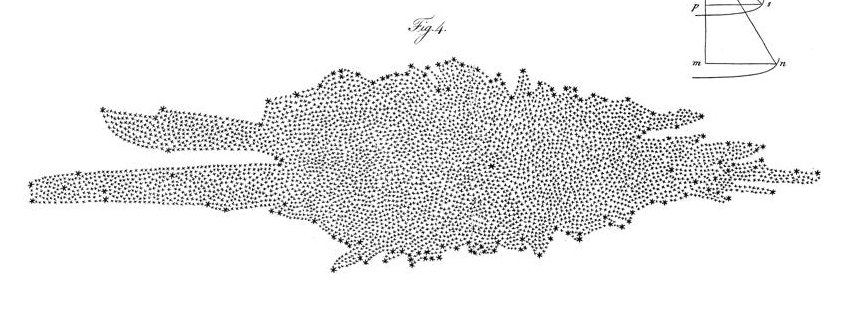
\includegraphics[width=1.0\textwidth]{./figures/1_introduction/Herschel_Model.png}
	
	\caption{\small{Modelo de William Herschel para nuestra galaxia, basado
	en un conteo de estrellas y la asunción de igual luminosidad \cite{Herschel1785}.}}
	
	\label{fig:HerschelModel}
\end{figure}
%.........................................................................


Otra importante cuestión observacional que estaba emergiendo en esa época
es sobre la existencia de otros \textit{universos islas} tal como el nuestro.
Era ya bien conocida la existencia de cuerpos extendidos en el cielo que no
se acomodaban satisfactoriamente a la definición de estrellas o planetas,
tales como nebulosas, discos planetarios y galaxias. Incluso William Herschel
y su hijo John Herschel contribuyeron con la realización de un gran catálogo
(para la época) de cuerpos extendidos conocido como \textit{Catálogo de 
Nebulosas y Cúmulos de Estrellas} y una versión expandida terminada por
John Dreyer en 1888, \textit{Nuevo Catálogo General de Nebulosas y Cúmulos
de Estrellas}, los cuales junto con el \textit{Índice de Catálogos} de 
1895 y 1908 constituyen una amplia colección de cuerpos ampliamente usados
en la astronomía actual, referidos con sus abreviaciones en inglés \textit{NGC}
y \textit{IC} respectivamente \cite{longair2008}. A pesar de todos estos
logros observacionales, la naturaleza real de estos objetos era un completo 
misterio, especialmente si ellos eran objetos dentro de nuestra propia 
galaxia o eran sistemas completamente independientes.


Esta última cuestión permaneció hasta el siglo veinte y junto con el tamaño
real del universo constituyeron los dos grandes temas tratados en el bien
conocido \textit{Gran Debate}, también denominado \textit{Debate de 
Shapley-Curtis}. Un importante evento en la historia de la astronomía donde
los astrónomos Harlow Shapley y Herber Curtis dieron respectivamente 
diferentes argumentos a favor y en contra de la pertenencia de esos objetos
a nuestra galaxia y si la Vía Láctea era todo nuestro universo. A pesar de 
todo, sus argumentos fueron poco concluyentes y la solución al estos 
problemas debió esperar hasta 1924 cuando Edwin Hubble midió la distancia
a la galaxia de Andrómeda (M31 o NGC 224) y demostró incuestionablemente 
la verdadera naturaleza extragaláctica de este objeto, y en años posteriores
para los demás. Este logro junto con la verificación observacional de la 
expansión del universo (también debida a Hubble) fueron el comienzo de la 
cosmología observacional moderna.


También sucedió en el siglo veinte un evento clave para las modernas 
\textit{ciencias de la gravedad}, Albert Einstein formuló su Teoría
General de la Relatividad, cambiando completamente la concepción previa
de espacio y tiempo, llegando así a nuestra compresión actual de la 
cosmología.


%*************************************************************************




%*************************************************************************
%The current cosmology picture
\section{La Cosmología Actualmente}
\label{sec:TheCurrentCosmologyPicture}


Las bases teóricas para la relatividad general comenzaron a surgir con el 
auge de las geometrías no Euclidianas en el siglo diecinueve y comienzos 
del veinte cuando fue demostrado que el quinto postulado de Euclides no 
era necesario para construir geometrías autoconsistentes, llegando así a las
geometrías no planas (ver figura \ref{fig:NonEuclidean}). En especial fueron 
destacables los trabajos de Nikolai Lobachevsky (padre de las geometrías 
no Euclideas) y Bernhard Riemman, fundador de la geometría Riemanniana.


%.........................................................................
%Herschel Model of Our Galaxy
\begin{figure}[htbp]
	\centering
	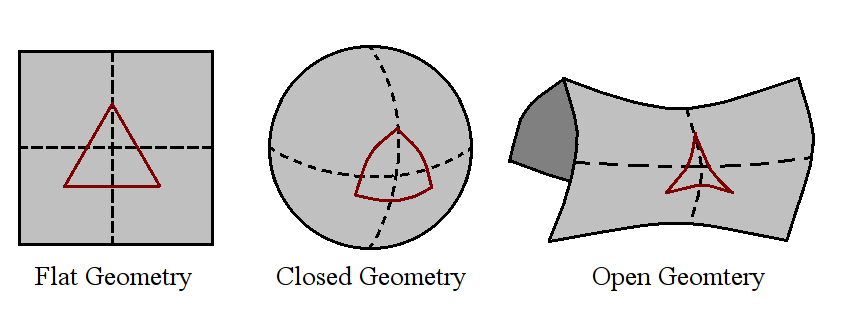
\includegraphics[width=0.9\textwidth]{./figures/1_introduction/Non_Euclidean.png}
	
	\caption{\small{Diferentes geometrías con variación del quinto postulado 
	de Euclides.}}
	
	\label{fig:NonEuclidean}
\end{figure}
%.........................................................................



A pesar de que estos primeros desarrollos en geometría había dado lugar a
fuertes discusiones sobre el tipo de geometría del universo, los conceptos de 
espacio y tiempo eran aún interpretados de forma absoluta y más aún, su 
conexión con la gravedad completamente ignorada. Es por esta razón que 
la formulación de la Relatividad General abrió la puerta a toda nuestra
comprensión moderna.


Una vez obtenidas las ecuaciones de campo métrico de la Relatividad General
fue posible construir modelos globales y autoconsistentes del universo. Un
primer intento se debe al propio Einstein, quién formuló con influencia 
de su propia creencia un modelo de universo estático y cerrado. Para lograr 
esto debió hacer uso de la bien conocida constante cosmológica para 
contrarrestar la expansión/contracción natural de las soluciones que dan 
la teoría.


Pocos años después	




%*************************************************************************




%*************************************************************************
%Cosmological observations
\section{Observaciones Cosmológicas}
\label{sec:CosmologicalObservations}
	
%*************************************************************************

%---------------------- theoretical frame -----------------------
%qqqqqqqqqqqqqqqqqqqqqqqqqqqqqqqqqqqqqqqqqqqqqqqqqqqqqqqqqqqqqqqqqqqqqqqqq
%Quote
\begin{savequote}[50mm]
‘‘The Cosmos is all that is or was or ever will be. Our feeblest contemplations 
of the Cosmos stir us: there is a tingling in the spine, a catch in the voice, 
a faint sensation, as if a distant memory, of falling from a height. We know 
we are approaching the greatest of mysteries.’’

\qauthor{Carl Sagan}
\end{savequote}
%qqqqqqqqqqqqqqqqqqqqqqqqqqqqqqqqqqqqqqqqqqqqqqqqqqqqqqqqqqqqqqqqqqqqqqqqq




%#########################################################################
\chapter{Theoretical Framework in Cosmology}
\label{cha:Theoretical Framework}


%Reviewed
The aim of this chapter is to cover, in a self-contained and summarized 
way, all the theoretical framework needed for the study of the large-scale
universe. From the simplest models of the universe given by Friedman's 
solutions, the theory of perturbations for the formation of complex 
structures like galaxies and galaxy clusters, until the schemes to 
quantify the cosmic web.



%#########################################################################




%*************************************************************************
%Isotropic and homogeneous universe
\section{Isotropic and Homogeneous Universe}
\label{sec:IsotropicAndHomogeneousUniverse}


%Reviewed
The two big pillars of the modern cosmology are the cosmological principle
and the theory of the general relativity. The first one is a principle 
where it is assumed that the universe is isotropic and homogeneous at very
large scales, while the second one gives the theoretical support needed in 
order to understand properly the relation between the matter content of 
the universe and the structure of the space-time.


%Reviewed
As it has been evidenced by observations of large-scale structures and the 
CMB, the universe appears to be isotropic and homogeneous at large scales,
which is in agreement with the cosmological principle. Moreover, this fact
simplifies quite enough the complex tensorial formulation of the general
relativity, thereby allowing finally leading to the Friedmann's equations.



	%---------------------------------------------------------------------
	%Curved space metric
	\subsection{Metric of Curved Spaces}
	\label{subsec:MetricOFCurvedSpaces}
	%---------------------------------------------------------------------

	
%Reviewed
In the construction of an isotropic and homogeneous model of universe, it 
is necessary to establish an adequate metric which describes it properly. 
An illustrative example that could be generalized is a 2D spherical 
surface, which clearly satisfies the criteria of homogeneity and isotropy.



%.........................................................................
%2D sphere
\begin{figure}[htbp]
	\centering
	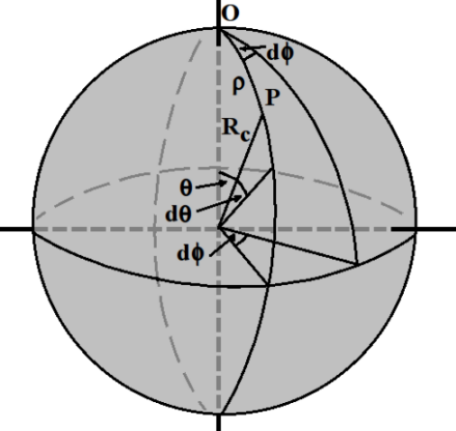
\includegraphics[width=0.5\textwidth]
	{./figures/2_theoretical_framework/2D_Sphere.png}
	
	\caption{\small{Metric of a spherical surface.}}
	
	\label{fig:2sphere}
\end{figure}
%.........................................................................


%Reviewed
A line element over the surface shown in Figure \ref{fig:2sphere} can
be described as


%Reviewed
%.........................................................................
%Line element on the sphere
\[ dl^2 = d\rho^2 + R_c^2 \sin^2 \pr{ \frac{\rho}{R_c}}d\phi^2 \]
%.........................................................................
where it have been introduced a new length coordinate over the surface, 
defined as $\rho = \theta R_c$ and $R_c$ is the curvature radius of the 
sphere. Another very convenient way to rewrite this expression, and that 
allowing a very useful generalization, it is reached defining the curvature
parameter $k$ and the coordinate $r = \sin (\rho/a)$, obtaining:


%Reviewed
%.........................................................................
%Line element on the sphere with time-dependent curvature
\[ dl^2 = a^2(t) \cor { \frac{dr^2}{1-kr^2} + r^2 d\phi^2 } \]
%.........................................................................
with $k = -1$ and it is assumed a time-dependent curvature radius $R_c = 
a(t)$. The metric in this case is 3D and is obtained by replacing the 
differential element of angle $d\phi^2$ by the solid angle differential 
$d\Omega^2 = d\theta^2 + \sin^2\theta d\phi^2$.


 
%.........................................................................
%Line element on the 3-sphere
\eq{eq:LineElement3D}
{ dl^2 = a^2(t) \cor { \frac{dr^2}{1-kr^2} + r^2 (d\theta^2 + 
\sin^2\theta d\phi^2)} }
%.........................................................................


%Reviewed
Finally, time is included, so the space-time interval for the metric of
isotropic and homogeneous curved spaces is:



%.........................................................................
%Interval element on the 3-sphere
\eq{eq:IntervalCurvedSpaces}
{ ds^2 = c^2 dt^2 - a^2(t) \cor { \frac{dr^2}{1-kr^2} + r^2 (d\theta^2 + 
\sin^2\theta d\phi^2)} }
%.........................................................................


%Reviewed
The direct generalization of this expression consists in varying the 
different values of the curvature parameter $k$ in order to obtain the 
metric of flat ($k = 0$), spherical closed ($k = -1$) or opened spaces
($k = 1$), as it is shown in \cite{longair2008} or \cite{padmanabhan1995}.


\
%.........................................................................
%Curved Spaces
\begin{figure}[htbp]
	\centering
	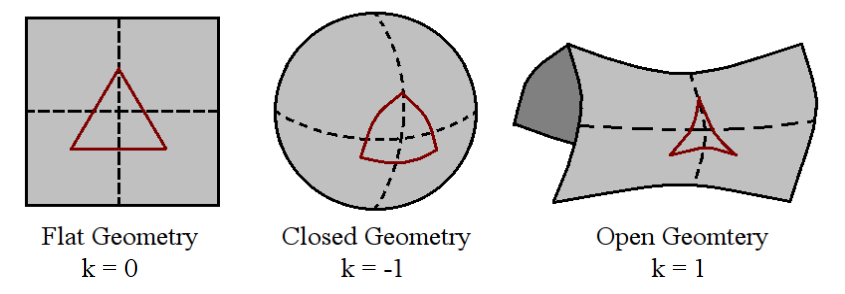
\includegraphics[width=0.9\textwidth]
	{./figures/2_theoretical_framework/Curved_Spaces.png}

	\caption{\small{Curved spaces according to the curvature parameter.}}
	
	\label{fig:CurvedSpaces}
\end{figure}
%.........................................................................
\

%Reviewed
An alternative way to rewrite the metric is introducing two changes of 
coordinates defined as



%.........................................................................
%Xi variable
\[ \chi = \int \frac{ dr'}{\sqrt{1 - k r'^2}}\]
%.........................................................................


%Reviewed
%.........................................................................
%Proper time
\[ \tau = \int \frac{ c dt'}{a(t')}\]
%.........................................................................
where each one is respectively interpreted as a length coordinate over the 
hypersurface that defines the space ($\chi$) and as the proper time 
measured locally ($\tau$). It is obtained the next expressions for the 
metric



%.........................................................................
%Interval element generalized
\eq{eq:IntervalCurvedSpacesAltern1}
{ ds^2 = c^2 dt^2 - a^2(t) \cor { d\xi^2 +  f^2_k(\xi)(d\theta^2 + 
\sin^2\theta d\phi^2)} }
%.........................................................................


%Reviewed
%.........................................................................
%Interval element generalized
\eq{eq:IntervalCurvedSpacesAltern2}
{ ds^2 = \bar a^2 (\tau)\cor{ d\tau^2 - d\xi^2 -  f^2_k(\xi)(d\theta^2 + 
\sin^2\theta d\phi^2)} }
%.........................................................................
where the function $f_k(\chi)$ is defined according to the value of the 
curvature parameter.



%.........................................................................
%Curvature Function
\eq{eq:CurvatureFunction}
{ f_k(\chi) = \left\{  \matrix{	
\sin \chi	&	k = 1		\cr 
\chi 		& 	k = 0 		\cr	
\sinh \chi 	& 	k = -1 		\cr } \right.  }
%.........................................................................


%Reviewed
In spite of the derived expressions for the metric 
\ref{eq:IntervalCurvedSpaces} \ref{eq:IntervalCurvedSpacesAltern1} and
\ref{eq:IntervalCurvedSpacesAltern2} are completely equivalent, the usage
of one or another depends on the specific problem. Especially the 
expression \ref{eq:IntervalCurvedSpacesAltern1} is usually more used and
is defined as the Friedmann's metric.


%Reviewed
It could be shown that in Riemannian manifolds \footnote{A Riemannian 
manifold is a space where it can be defined (well-defined) a metric.},
the space-time interval is expressed in terms of the metric tensor as
\cite{weinberg1972}


%Reviewed
%.........................................................................
%Metric-Interval relation
\[ ds^2 = g_{\mu \nu}dx^\mu dx_\nu \]
%.........................................................................
where it has been introduced the cuadrivector $x^\mu = 
(ct, r, \theta, \phi)$.


%Reviewed
Due to the assumption of isotropy and homogeneity, the metric tensor must
be diagonal, furthermore, comparing with the expression 
\ref{eq:IntervalCurvedSpaces}, it is possible to obtain the next explicit 
form



%.........................................................................
%MetricTensor
\eq{eq:MetricTensor}
{g_{\mu \nu} = \pr{ \matrix{ 
1		&				0			&		0			&				0				\cr
0		&	-a^2(t)(1 - kr^2)^{-1}	&	 	0			&				0				\cr
0		&				0			&	-a^2(t)r^2		&				0				\cr
0		&				0			&		0			&	-a^2(t)r^2 \sin^2 \theta } }}
%.........................................................................


%Reviewed
From this metric and the Einstein's field equations, it is possible to 
build simple models of the universe, such as it shall be shown in the 
subsection \ref{subsec:GeneralRelativityAndFriedmannEquations}.



			%-------------------------------------------------------------
			%Measuring distances
			\subsubsection*{Measuring distances}
			%-------------------------------------------------------------


%Reviewed
Once defined the metric of curved spaces, it is very useful to introduce
some concepts related with distances, which are used recurrently 
\cite{longair2008}. For the sake of simplicity it will be assumed a flat 
metric ($k = 0$).


%Reviewed
\begin{itemize}
%Comovil Radial Distance..................................................
\item \textit{\textbf{Comoving radial distance:}} by definition, a light
signal has an associated null interval, i.e. $ds^2 = 0$. Using the 
expression \ref{eq:IntervalCurvedSpaces} for the metric, it is obtained


%Reviewed
%.........................................................................
%Comovil Distance
\eq{eq:ComovilDistance}
{ r = \int_t^{t_0} \frac{ cdt'}{a(t')} = \int_a ^1 \frac{ c da}{a \dot a} }
%.........................................................................
where the specific form of $a(t)$ depends on the specific chosen cosmology
(see subsection \ref{subsec:SimpleSolutionsOfTheUniverse}) and $t_0$ is the
reference time, which is taken as the current age of the universe.


%Reviewed
Due to the assumption of an expanding metric, the distance between two 
objects depends on the time in which the measurement is performed. 
Moreover, the distance cannot be determined from a beam of light since
light has a finite velocity \footnote{$c=299\ 792\ 458$ m/s}. Because of 
that, it must be performed a projection on the light-cone traced by the 
beam in the current time, such as it is made in the expression 
\ref{eq:ComovilDistance}. The latter allows interpreting $r$ as the 
distance to an object in the current time, and it is quite different to
the apparent distance which corresponds to the time when the object in 
question emitted the observed light.


%Reviewed
%Proper Radial Distance..................................................
\item \textit{\textbf{Proper radial distance:}} by virtue of the 
definition of scale factor, to obtain the distance to an object in any 
time, it is enough to multiply the comoving distance by the scale factor 
evaluated in the same time, that is



%.........................................................................
%Proper Distance
\eq{eq:ComovilDistance}
{ r_{\submath{prop}} = a(t)\int_t^{t_0} \frac{ cdt'}{a(t')} = 
a\int_a ^1 \frac{ c da}{a \dot a} }
%.........................................................................	


%Reviewed
%Particle Horizon........................................................
\item \textit{\textbf{Particle horizon:}} considering a beam travelling 
through vacuum since the beginning of all time, at $t=0$; the maxim proper
distance that could be travelled by the light in a time $t$ is denominated 
particle horizon and determines all regions in the universe that could 
have been causally connected in that time. 



%.........................................................................
%Particle Horizon distance
\eq{eq:HorizonDistance}
{ r_{\submath{H}} = a(t)\int_0^{t} \frac{ cdt'}{a(t')} = 
a\int_0 ^a \frac{ c da}{a \dot a} }
%.........................................................................

\end{itemize}
	%---------------------------------------------------------------------
	%General relativity and Friedmann equations
	\subsection{General Relativity and Friedmann's Equations}
	\label{subsec:GeneralRelativityAndFriedmannEquations}
	%---------------------------------------------------------------------
	

%Reviewed
The Einstein's field equations of the general relativity play a fundamental
role since they express explicitly the relation between the matter 
content of the universe and the local geometry of the space-time.


%Reviewed
%.........................................................................
%EinsteinEquations
\eq{eq:EinsteinEquations}
{ R_{\mu \nu} - \frac{1}{2}R - g_{\mu \nu}\Lambda = 
\frac{8\pi G}{c^4}T_{\mu \nu} }
%.........................................................................
or equivalently


%Reviewed
%.........................................................................
%Einstein Equations Alternative
\eq{eq:EinsteinEquationsAltern}
{ R_{\mu \nu} + g_{\mu \nu}\Lambda = 
\frac{8\pi G}{c^4}\pr{T_{\mu \nu} - \frac{1}{2}T g_{\mu \nu}} }
%.........................................................................
where $T$ is the trace of the energy-momentum tensor (see 
\ref{eq:MomentumEnergyTensor}), $R_{\mu \nu}$ the Ricci curvature tensor
and $R$ the scalar curvature. The last two terms are calculated from 
different traces of the Riemann curvature tensor, as $R_{\mu \nu} = 
R^\eta_{\ \mu \eta \nu}$ and $R = R^{\mu}_{\ \mu}$. For convenience, it
has been introduced the term associated with the cosmological constant, 
which will be used below to calculate different models of the universe 
with dark energy contribution.


%Reviewed
The Riemann curvature tensor quantifies deviations of the metric of curved 
space-times with respect to the Euclidean metric and allows to determinate
completely the geometrical properties like the local curvature, different 
measures of distances and angles, etc. \cite{weinberg1972}. This tensor is
built from the Levi-Civita connection as


%Reviewed
%.........................................................................
%Riemann Tensor
\eq{eq:RiemannTensor}
{ R^\mu_{\ \nu \alpha \beta} = 
\Gamma^\mu_{\ \nu \alpha, \beta} -  
\Gamma^\mu_{\ \nu \beta, \alpha} + 
\Gamma^\mu_{\ \sigma \alpha}\Gamma^\sigma_{\ \nu \beta}-
\Gamma^\mu_{\ \sigma \beta}\Gamma^\alpha_{\ \nu \alpha}}
%.........................................................................
with the Levi-Civita connection defined from the metric as



%.........................................................................
%Afin Connection
\eq{eq:AfinConnection}
{ \Gamma^\nu _{\ \alpha \beta}  = \frac{1}{2}g^{\mu \sigma}
\pr{ g_{\sigma \alpha, \beta} + g_{\sigma \beta, \alpha} -
g_{\alpha \beta, \sigma} } }
%.........................................................................


%Reviewed
The right-hand side of the equation \ref{eq:EinsteinEquations} contains
the energy-momentum tensor $T_{\mu \nu}$, which characterizes the density
and the matter-energy flux of the universe. By virtue of the cosmological 
principle, this tensor must also be diagonal and if, furthermore, it is 
assumed an ideal fluid model, the next form is obtained



%.........................................................................
%MomentumEnergyTensor
\eq{eq:MomentumEnergyTensor}
{T^\mu_{\ \nu} = \pr{ \matrix{ 
c\rho^2	&	0	&	0	&	0				\cr
0		&	-P	&	0	&	0				\cr
0		&	0	&	-P	&	0				\cr
0		&	0	&	0	&	-P } }}
%.........................................................................


%Reviewed
Finally, using the equations \ref{eq:MetricTensor}, 
\ref{eq:EinsteinEquationsAltern} and \ref{eq:MomentumEnergyTensor}, it is 
possible to reduce the complex system of tensorial equations to two scalar
coupled equations which are usually called Friedmann's equations 
\cite{longair2008}. These equations describe completely the evolution of
an isotropic and homogeneous universe in terms of the scale factor $a(t)$ 
(see equation \ref{eq:LineElement3D})



%.........................................................................
%Friedmann Equation 1
\eq{eq:FriedmannEquation1}
{ \frac{\ddot a}{a} = -\frac{4\pi G}{3}\pr{\rho + \frac{3P}{c^2}}
+ \frac{c^2 \Lambda}{3}}
%.........................................................................


%.........................................................................
%Friedmann Equation 2
\eq{eq:FriedmannEquation2}
{ \frac{\ddot a}{a} + 2\frac{\dot a^2}{a^2} + 2\frac{c^2 k}{a^2} =
4\pi G \pr{ \rho - \frac{P}{c^2} } + c^2 \Lambda}
%.........................................................................


%Reviewed
In order to solve this equation system in terms of $a(t)$ and thereby 
obtaining the evolution of the scale factor, it is necessary to know the 
explicit time-dependent expression of the density $\rho$ and the pressure
$P$, or equivalently, the dependence on the scale factor. This must be done
for each type of energy-matter of the universe. A detailed derivation of
these explicit expressions could be found in \cite{longair2008} and they
are summarized in Table \ref{tab:PropertiesDependence}.



%.........................................................................
%Table of dependences of Matter-Energy content of the universe with a
\begin{table}[htbp]
\centering
\begin{tabular}{|c|c|c|c|} \hline
\cellc{\textbf{Property}} 	& 
\cellc{\textbf{Density}} 	&
\cellc{ \textbf{Pressure}}	& 
\cellc{\textbf{Temperature}}		\\ \hline

& & &  \\
\textbf{Matter}& $\rho = \rho_0 a^{-3}(t)$ & $p = p_0 a^{-5}(t)$ & $T = T_0 a^{-2}(t)$ \\ 
\small{(baryonic + dark)} & & &  \\ \hline
& & &  \\
\textbf{Radiation }& $\rho = \rho_0 a^{-4}(t)$ & $p = p_0 a^{-4}(t)$ & $T = T_0 a^{-1}(t)$ \\ 
\small{(+ relativistic matter)} & & &  \\ \hline
& & &  \\
\textbf{Vacuum }& $\rho = \rho_0 $ & $p = p_0 $ & $-$ \\ 
& & &  \\ \hline
\end{tabular}
\caption{Dependence of some quantities on the scale factor $a(t)$
\cite{longair2008}.}
\label{tab:PropertiesDependence}
\end{table}
%.........................................................................


%Reviewed
By convention, it has been taken the current scale factor as $a_0 = a(t_0) 
= 1$ and the reference values are defined as $\rho_0 = \rho(a_0)$, $P_0 = 
P(a_0)$ and $T_0 = T(a_0)$. Using the Friedmann's equations, defining the
Hubble parameter as $H(t) = \dot a/ a$ and the vacuum density as 
$\rho_\Lambda = c^2\Lambda/8\pi G$, it is obtained



%.........................................................................
%Pre Hubble Equation
\[ \pr{ \frac{\dot a}{a} }^2 = H^2(t) = \frac{ 8\pi G}{3}
\cor{ \rho_{m}\frac{1}{a^{3}} + \rho_{r}\frac{1}{a^{4}} + \rho_{\Lambda} }
- \frac{ c^2 k }{a^2} \]
%.........................................................................


%Reviewed
Evaluating this expression in the current epoch $H(t_0) = H_0$, with $H_0$
the Hubble constant and defining the critical density $\rho_c$ as the 
density that the universe must have in order to be flat.


%Reviewed
%.........................................................................
%Critical Density
\eq{eq:CriticalDensity}
{ \rho_c = \frac{3H_0^2}{8\pi G} }
%.........................................................................
it leads to the equation of evolution for the Hubble parameter


%Reviewed
%.........................................................................
%Hubble Equation
\eq{eq:HubbleEquation}
{ H^2(t) = H_0^2 \cor{ 
(1 - \Omega_0)\frac{1}{a^2} +  
\Omega_m \frac{1}{a^3} +
\Omega_r \frac{1}{a^4} +
\Omega_\Lambda} }
%.........................................................................
where it has been introduced the density parameters $\Omega_i$, defined
as the current density of the i-th specie in the current epoch, normalized 
with the critical density \ref{eq:CriticalDensity}, and $\Omega_0 = 
\sum_i \Omega_i$. These density parameters along with the Hubble constant
are part of the free parameters of the theory and must be determined by 
observations. This allows to characterize different particular cosmologies
\footnote{\textit{Cosmology} must be understood in this context as a 
specific solution of the Friedmann's equations.}



	%---------------------------------------------------------------------
	%Simple solutions of the universe
	\subsection{Simple Solutions of the Universe}
	\label{subsec:SimpleSolutionsOfTheUniverse}
	%---------------------------------------------------------------------


%Reviewed
Although in this stage it has not been introduced the complete formalism 
of small perturbations and structure formation, the set of equations
\ref{eq:FriedmannEquation1}, \ref{eq:FriedmannEquation2} and 
\ref{eq:HubbleEquation} leads to a first and rough understanding of the
evolution of the Universe.


%Reviewed
In this subsection will be presented some analytic solutions to the 
Friedmann's equations. In spite of the ideal assumptions on which are
based, in some cases, they can be used as approximations in some stages
of evolution of the universe, thus allowing a physical understanding more 
adequate than exact numerical solutions.



			%-------------------------------------------------------------
			%Einstein-de Sitter Universe
			\subsubsection*{Einstein - de Sitter Universe}
			%-------------------------------------------------------------


%Reviewed
The Einstein-de Sitter Universe is a cosmological model with a flat metric
and composed entirely of matter, this implies that $\Omega_0 = \Omega_m = 1$ 
and $k=0$. Applying this in equation \ref{eq:HubbleEquation}, it is obtained
the next expression



%.........................................................................
%EinsteindeSitter
\eq{eq:EinsteindeSitter}
{ H^2(t) = \pr{\frac{\dot a}{a}}^2 = H_0^2 \frac{1}{a^3} }
%.........................................................................


%Reviewed
Integrating, it leads to the explicit time-dependent solution for the 
scale factor



%.........................................................................
%EinsteindeSitterSolution
\eq{eq:EinsteindeSitterSolution}
{ t(a) = \frac{ 2}{3H_0} a ^{3/2} }
%.........................................................................


%Reviewed
Although in this case it is possible to obtain the explicit form of $a(t)$,
most of the time it is only possible to have the implicit solution $t(a)$.
Another very useful way to describe this solution is by using the redshift
$z$, which is related with the scale factor as \cite{longair2008}


%Reviewed
%.........................................................................
%Redshift
\eq{eq:Redshift}
{ z + 1 = \frac{ a_0}{a} }
%.........................................................................
to finally obtain



%.........................................................................
%EinsteindeSitterSolutionZ
\eq{eq:EinsteindeSitterSolutionZ}
{ t(a) = \frac{ 2}{3H_0} (1+z) ^{-3/2} }
%.........................................................................


%Reviewed
This solution is quite close to the real behaviour of the universe in the 
matter-dominated epoch, between $70000$ and $5$ millions of years after 
the Big Bang \cite{padmanabhan1995}.



			%-------------------------------------------------------------
			%Radiation Dominated Universe
			\subsubsection*{Radiation-Dominated Universe}
			%-------------------------------------------------------------


%Reviewed
In this case, it will be assumed that the universe is radiation-dominated, 
that is $\Omega_0 = \Omega_r$, but not necessarily flat. The Friedmann's 
equations lead to the next expression



%.........................................................................
%Radiation Universe
\eq{eq:RadiationUniverse}
{ H^2(t) = \pr{\frac{\dot a}{a}}^2 = H_0^2 \cor{ 
(1 - \Omega_r)\frac{1}{a^2} +  \Omega_r \frac{1}{a^4}} }
%.........................................................................


%Reviewed
Integrating this expression, it is obtained the next implicit solution for
the scale factor


%Reviewed
%.........................................................................
%Radiation Universe Solution
\eq{eq:RadiationUniverseSolution}
{ t = \left\{  \matrix{ 
H_0^{-1}(\Omega_r - 1)^{-1}\pr{ \Omega_r^{1/2} - 
\cor{a^2(1-\Omega_r) + \Omega_r}^{1/2} } & \Omega_r \neq 1 \cr
H_0^{-1} a^2/2 & \Omega_r = 1} \right. }
%.........................................................................
or in terms of redshift



%.........................................................................
%Radiation Universe Solution Z
\eq{eq:RadiationUniverseSolutionZ}
{ t = \left\{  \matrix{ 
H_0^{-1}(\Omega_r - 1)^{-1}\pr{ \Omega_r^{1/2} - 
\cor{(1+z)^{-2}(1-\Omega_r) + \Omega_r}^{1/2} } & \Omega_r \neq 1 \cr
H_0^{-1} (1+z)^{-2}/2 & \Omega_r = 1} \right. }
%.........................................................................


%Reviewed
This solution is useful as an approximation for the radiation-dominated 
epoch, which happened from the big bang until the recombination epoch, 
approximately $380 000$ years after the big bang, or equivalently in a
redshift of $z = 1100$ \cite{padmanabhan1995}.



			%-------------------------------------------------------------
			%Vacuum Dominated Universe
			\subsubsection*{Vacuum-dominated Universe}
			%-------------------------------------------------------------
		

%Reviewed	
This type of hypothetical universe is completely vacuum-dominated, or
equivalently dominated by the cosmological constant. Making $\Omega_0 = 
\Omega_\Lambda$ in the Friedmann's equations, it is obtained
			


%.........................................................................
%Vacuum Universe
\eq{eq:VacuumUniverse}
{ H^2(t) = \pr{\frac{\dot a}{a}}^2 = H_0^2 \cor{ 
(1 - \Omega_\Lambda)\frac{1}{a^2} +  \Omega_\Lambda} }
%.........................................................................


%Reviewed	
Solving for $t(a)$


%Reviewed
%.........................................................................
%Vacuum Universe Solution
\eq{eq:VacuumUniverseSolution}
{ t = \frac{1}{H_0^2 \Omega_\Lambda^{1/2}}
\ln\cor{ a \pr{ \frac{\Omega_\Lambda}{1 - \Omega_\Lambda} }^{1/2} +
\pr{ 1 + \frac{\Omega_\Lambda}{1 - \Omega_\Lambda}a^2 }^{1/2} } }
%.........................................................................
and using the redshift



%.........................................................................
%Vacuum Universe Solution Z
\eq{eq:VacuumUniverseSolutionZ}
{ t = \frac{1}{H_0^2 \Omega_\Lambda^{1/2}}
\ln\cor{ \frac{1}{1+z} \pr{ \frac{\Omega_\Lambda}{1 - \Omega_\Lambda} }^{1/2} +
\pr{ 1 + \frac{\Omega_\Lambda}{1 - \Omega_\Lambda}\frac{1}{\pr{1+z}}^2 }^{1/2} } }
%.........................................................................


%Reviewed
This solution is very interesting because, unlike the previous solutions, 
is only valid for values of the density parameter within the range 
$0<\Omega_\Lambda <1$. This implies that it is not possible to have a  
universe with flat or hyperbolic geometry when it is vacuum-dominated.
Another aspect equally remarkable is the concavity of the scale factor 
$a(t)$ obtained from \ref{eq:VacuumUniverseSolution} (see figure 
\ref{fig:Cosmologies}), which shows an accelerated expansion of the 
universe. This characteristic is only possible when there is a non-null 
term associated to the vacuum energy.


%Reviewed
Finally and like the previous solutions, the expression 
\ref{eq:VacuumUniverseSolution} can be used as an approximation for the
vacuum-dominated epoch of the universe, which lasts from the end of the
matter-dominated epoch, $5$ millions of years after the big bang, until 
nowadays \cite{longair2008}.



			%-------------------------------------------------------------
			%WMAP7 Universe
			\subsubsection*{WMAP7 Universe}
			%-------------------------------------------------------------
			
			
%Reviewed
The set of parameters associated to the standard cosmological model has 
been measured on several occasions by different spacecraft missions (see
section \ref{sec:CosmologicalObservations}). Among those measurements it 
is notable the one conducted by WMAP. The data obtained after seven years
of observation (WMAP7) are adopted in this work \cite{WMAP7}. Among the 
cosmological parameters measured are the Hubble constant and the density
parameters $\Omega_i$. Taking the values given in Table 
\ref{tab:CosmologicalParameters} and for simplicity assuming $\Omega_0 = 1$
it is possible to integrate the Friedmann's equations

			
%Reviewed	
%.........................................................................
%WMAP Universe
\eq{eq:WMAPUniverse}
{ H^2(t) = H_0^2 \cor{ 
\Omega_m \frac{1}{a^3} +
\Omega_r \frac{1}{a^4} +
\Omega_\Lambda} }
%.........................................................................
to obtain


%.........................................................................
%WMAP Universe
\eq{eq:WMAPUniverse}
{ t = \frac{1}{H_0}\int _0 ^{a}\cor{ 
\Omega_m \frac{1}{a'} + 
\Omega_r \frac{1}{a'^2} +
\Omega_\Lambda a'^2 }^{-1/2}da' }
%.........................................................................

\
%.........................................................................
%Friedmann Solutions
\begin{figure}[htbp]
	\centering
	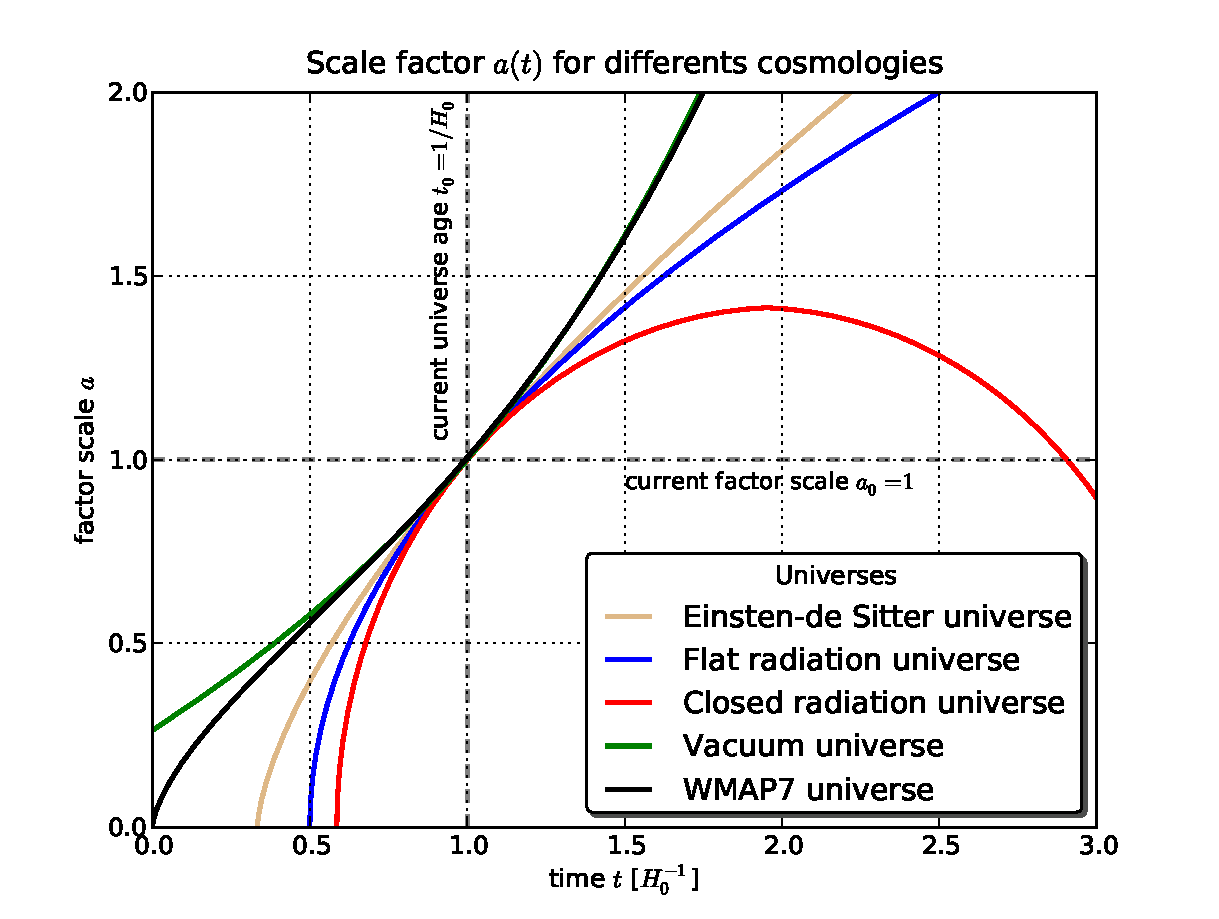
\includegraphics[width=0.9\textwidth]
	{./figures/2_theoretical_framework/Friedmann_Solution.pdf}

	\caption{\small{Different solutions of the universe according to the
	Friedmann's equations.}}
	
	\label{fig:Cosmologies}
\end{figure}
%.........................................................................
\

%Reviewed
It is possible to obtain an analytic solution of this integral in terms of
elliptic functions, but for simplicity it is chosen the numerical solution.
In Figure \ref{fig:Cosmologies} is shown the solution for a WMAP7 
universe and it is compared with other cosmologies, derived previously.


%Reviewed
An interesting characteristic of the solution for the WMAP7 universe is 
the change of concavity (black curve in Figure \ref{fig:Cosmologies}), 
which indicates a transition from the matter/radiation-dominated epoch
to an accelerated expanding regime associated to the vacuum energy.
Another important aspect is the prediction of the age of the universe.
Taking into account the previously defined normalization for the scale
factor $a(t_0) = a_0$, it is straightforward to see that $t_0 = H_0^{-1} 
\approx 13.75 \times 10^9$ years. Other cosmologies under the same 
normalization predict different ages, since larger values such as a 
vacuum-dominated universe, until smaller and even a collapse time (usually
known as big crunch time) such as a radiation-dominated and closed 
universe.



%*************************************************************************




%*************************************************************************
%Linear Structure Formation
\section{Linear Regime of Structure Formation}
\label{sec:LinearStructureFormation}


%Reviewed
The previous section deals about the universe as a whole, assuming as 
valid the condition of isotropy and homogeneity. Although the real universe
has this asymptotic behaviour at very large scales, at smaller local scales
the behaviour is quite different, being even completely anisotropic and 
highly non-homogeneous. Life is certainly the most illustrative example of 
that, one of the highest non-linearities of the universe, and thus, 
planets, stars, galaxies, galaxy clusters, in the same decreasing order of 
inhomogeneity and anisotropy.


%Reviewed
The standard way to introduce these local structures in the universe is by
assuming as valid the solutions of the Friedmann's equations at very large 
scales, but considering inhomogeneities as perturbations of the model. 
First, in the linear regime, where the perturbations in the density field
are much smaller than the background mean density ($\delta \rho \ll 
\rho_b$), and after, in the non-linear regime, where the perturbations are
comparable or even larger ($\delta \rho \sim \rho_b$) (see section 
\ref{sec:NonLinearStructureFormation}).

 

	%---------------------------------------------------------------------
	%Newtonian Approximation
	\subsection{Newtonian Approximation}
	\label{subsec:Newtonian Approximation}
	%---------------------------------------------------------------------


%Reviewed
The frame of linear evolution can be presented in two ways. The first 
one is by considering a perturbative term in the energy-momentum tensor
$ \delta T_{\mu \nu}$ and linearizing the Einstein's field equations 
\ref{eq:EinsteinEquations} and finally solving for $\delta R_{\mu \nu}$



%.........................................................................
%Perturbative Einstein Equations
\eq{eq:PerturbativeEinsteinEquations}
{ \mathcal{L}( R_{\mu \nu}, \delta R_{\mu \nu} ) = 
\frac{8\pi G}{c^2}\pr{ T_{\mu \nu} + \delta T_{\mu \nu} } }
%.........................................................................


%Reviewed
Although this method is, rigorously, more adequate, it has an inconvenience
which makes it very complicated of applying. Non-perturbative terms are 
not necessarily small in all the coordinate systems, inclusively, they can 
reach values with the same order or even bigger than the background mean 
density \cite{padmanabhan1995}.


%Reviewed
The second method consists in assuming perturbations with a comoving size
smaller than the Hubble radius ($r_\delta \ll r_H \sim cH_0^{-1}$)
\footnote{The Hubble radius $r_H$ is a length unit that defines the 
order of magnitude of the size of the observable universe.}, thereby
being possible to neglect relativistic effects due to the curvature
of the space-time. Once this is done, it is possible to use a Newtonian
scheme to evolve perturbations of the background universe. This scheme
assumes that the matter content of the universe is a fluid described by
three basic equations of fluid mechanics. The first one is the continuity
equation, which expresses mass conservation in a fluid



%.........................................................................
%Continuity equation
\eq{eq:ContinuityEquation}
{ \dtot{\rho}{t} = - \rho \nabla \cdot \bds u }
%.........................................................................


%Reviewed
The second one, Euler's equation, characterizes the velocity field of the 
fluid, and physically it expresses the momentum conservation law


%.........................................................................
%Euler Equation
\eq{eq:EulerEquation}
{ \dtot{\bds u}{t} = -\frac{ \nabla P}{\rho} - \nabla \varphi }
%.........................................................................


%Reviewed
And finally the Poisson's equation, which is the non-relativistic version
of the Einstein's field equations and expresses the relation between the
matter content of the universe and sources of gravitational field.

	
	
%.........................................................................	
%Poisson Equation
\eq{eq:PoissonEquation}
{ \nabla^2 \varphi = 4\pi G \rho }
%.........................................................................	


%Reviewed
In order to complete the Newtonian frame of perturbations is necessary to 
include in the previous system of equations (\ref{eq:ContinuityEquation}, 
\ref{eq:EulerEquation} and \ref{eq:PoissonEquation}) the effect of the 
expansion of the universe by making a change of coordinates of the proper
distance $\bds x$ to comoving distance $\bds r$


%Reviewed
%.........................................................................	
%Changing Coordinate
\[\bds x = a \bds r\]
%.........................................................................	
this implies that



%.........................................................................	
%Changing Coordinate
\[\bds u = \dtot{\bds x}{t} = 
\frac{\dot a}{a}\bds x + \bds v = \dot a \bds r + \bds v\]
%.........................................................................	


%Reviewed
This way to rewrite $\bds u$ allows separating the contribution of the 
expansion of the universe ($\dot a/a \bds x$), also called Hubble's law,
from the component due to the movement of the fluid, called peculiar 
velocity field and it is defined as $\bds v = a \dot{ \bds r}$.


%Reviewed
For the sake of simplicity it is decomposed the density field of the fluid 
into two parts, the background contribution and a perturbative term, that 
is $\rho = \bar \rho + \delta\rho = \bar \rho( 1+ \delta )$, where $\delta$
is called the density parameter and is dimensionless. In the case of the 
gravitational potential $\varphi$, it is defined a new field given by 
$ \Phi = \phi + \ddot a a r^2/2$ \cite{longair2008}. With these 
considerations it is finally obtained the final set of equations for 
describing a fluid in the Newtonian frame.


%Reviewed
%.........................................................................	
%Fluid Equations
\begin{eqnarray}
%.........................................................................	
\label{eq:ContinuityEquationC}
\matrix{\mbox{\footnotesize{Continuity}} \cr \mbox{\footnotesize{equation}}} & &
\der{\delta}{t} = - \frac{1}{a}\nabla_r \cdot \cor{ (1+\delta)\bds v }\\
\nonumber{}
\\
%.........................................................................	
\label{eq:EulerEquationC}
\matrix{\mbox{\footnotesize{Euler's}} \cr \mbox{\footnotesize{equation}}} & &
\der{\bds v}{t} + \frac{\dot a}{a}\bds v + 
\frac{1}{a}\pr{ \bds v\cdot \nabla_r }\bds v = 
-\frac{\nabla_r P}{a \bar \rho(1+\delta)} - 
\frac{1}{a}\nabla_r \Phi \\
\nonumber{}
\\
%.........................................................................	
\label{eq:PoissonEquationC}
\matrix{\mbox{\footnotesize{Poisson's}} \cr \mbox{\footnotesize{equation}}} & &
\nabla^2_r \Phi = 4\pi G\bar \rho a^2 \delta
\end{eqnarray}
%.........................................................................	


%Reviewed
Until this stage it has not made explicit what type of matter-energy 
content is described by the above perturbative fluid equations (e.g. 
radiation, dark matter, dark energy). Taking into account the followed 
procedure to derive the previous system of equations, it can be noticed
that no \textit{a priori} assumption has been made about the explicit 
dependence of the state variables on the scale factor (see table 
\ref{tab:PropertiesDependence}), therefore they are valid for any of the
different species \footnote{Henceforth, each one of the different 
matter-energy contents that contributes to the momentum-energy tensor, 
will be called \textit{specie}.} present in the universe. Bearing in mind 
that the structures of the current universe are completely composed of 
matter, it will be only used the Newtonian frame for this specie.


%Reviewed
The physical quantities that must be determined by the fluid equations 
together with the Friedmann's equations are: the density parameter 
$\delta$, the peculiar velocity field $\bds v$, the effective potential
$\Phi$, the pressure $P$ and finally the scale factor $a$. It is then so 
clear that another extra equation is needed in order to get a completely
self consistent problem. This is reached by introducing an equation of 
state for the pressure. For simplicity it is assumed a mono-atomic gas
model for the matter, with an associated equation of state given by


%Reviewed
%.........................................................................	
%EOS equation
\eq{eq:EOSEquation}
{ \nabla_r P = c_s^2 \bar \rho \nabla \delta + 
\frac{2}{3}\bar T \rho \nabla s }
%.........................................................................	
where $c_s$ is the velocity of sound in the medium, $\overline T$ the 
background temperature and $s$ the specific entropy. Using this expression
along with \ref{eq:ContinuityEquationC} and \ref{eq:EulerEquationC}, it is
obtained the general equation for the evolution of the perturbations



%.........................................................................	
%Delta Evolution
\eq{eq:DeltaEvolution}
{ \der{^2 \delta}{t^2} + 2\frac{\dot a}{a} \der{\delta}{t} = 
4\pi G \bar \rho \delta + \frac{c_s^2}{2}\nabla^2 \delta +
\frac{2}{3}\frac{\overline T}{a^2}\nabla^2 s }
%.........................................................................	


%Reviewed
In the linear regime, $\delta \ll 1$, the modes of the density field 
evolve independently from each other, thus allowing decoupling the 
perturbations at different size scales. A very standard way to solve this 
type of problems is by using Fourier transform because in the reciprocal 
space the modes of the field are decoupled naturally.


%Reviewed
Since it has been assumed perturbations with characteristic lengths 
smaller than the Hubble's radius, the volume of the observable universe 
can be considered finite, and therefore decomposition of the fields 
in comoving coordinates becomes discrete, obtaining

 

%.........................................................................	
%Fourier Descomposition of Fields
\[  \delta(\bds r, t) =  \sum_{\bds k}\delta_{\bds k} e^{i \bds k \cdot \bds x} 
\ \ \ \ \ 
	\bds v(\bds r, t) =  \sum_{\bds k}\bds v_{\bds k} e^{i \bds k \cdot \bds x}\]
\eq{eq:FourierFields}
{  s(\bds r, t) =  \sum_{\bds k}s_{\bds k} e^{i \bds k \cdot \bds x} 
\ \ \ \ \ 
	\Phi(\bds r, t) =  \sum_{\bds k}\Phi_{\bds k} e^{i \bds k \cdot \bds x}}
%.........................................................................	


%Reviewed
If adiabatic perturbations are assumed, that is, perturbations that 
cannot interchange heat with their environment (the background universe) 
while they are evolving, the specific entropy must remain homogeneous and
therefore $\nabla_r s = 0$ \cite{longair2008}. Considering this and using
the previous decompositions of the fields, it is reached the next set of 
equations for evolving the modes of the density and peculiar velocity 
fields associated to the perturbations.



%.........................................................................	
%Modes Evolution Equation
\begin{eqnarray}
%.........................................................................	
\label{eq:ContinuityEquationCMode}
\dtot{^2 \delta_{\bds k}}{t^2} + 2\frac{\dot a}{a}\dtot{\delta_{\bds k}}{t} &=& 
\cor{ 4\pi G \bar \rho - \frac{c_s^2}{a^2}k^2 }\delta_{\bds k}\\
\nonumber{}
\\
%.........................................................................	
\label{eq:EulerEquationCMode}
- k^2 \Phi_{\bds k} &=& 4\pi G \bar \rho a^2 \delta_{\bds k}\\
\nonumber{}
\\
%.........................................................................	
\label{eq:PoissonEquationCMode}
\bds v_{\bds k} &=& \frac{i a \bds k}{k^2}\dtot{\delta_{\bds k}}{t}
\end{eqnarray}
%.........................................................................	


	%---------------------------------------------------------------------
	%Jeans Instability
	\subsection{Jeans Instability}
	\label{subsec:JeansInstability}
	%---------------------------------------------------------------------
	
	
%Reviewed
Solutions to the equation \ref{eq:ContinuityEquationCMode} for the modes
of the density field can be classified into two different families. The 
first one is a set of solutions where the amplitude of each mode oscillates
over time and does not collapse. The second family is a set of solutions 
where each mode grows up over time, collapsing and becoming highly 
non-linear ($\delta_k \gg 1$). A quite simple example that illustrates the
above discussed and can be generalized, involves taking perturbations in 
a static universe, that is $\dot a = 0$. Taking this into account, the 
equation \ref{eq:ContinuityEquationCMode} is rewritten as


%Reviewed
%.........................................................................	
%JeansEquation
\eq{eq:JeansEquation}
{\dtot{^2 \delta_{\bds k}}{t^2} -\omega_k^2 \delta_{\bds k} = 0,\ \ \ a=\mbox{cte}}
%.........................................................................	
where it has been defined the characteristic frequency $\omega_k$ as



%.........................................................................	
%JeansFrequency
\eq{eq:JeansFrequency}
{\omega_k^2 = \cor{\frac{c_s^2}{a^2}k^2 -  4\pi G \bar \rho} }
%.........................................................................	
	

%Reviewed
Expression \ref{eq:JeansEquation} is called Jeans equation and it has the
form of a wave equation. Based upon this, solutions can be classified 
according to the value of $\omega_k$, such as it has been said initially.


%Reviewed
%.........................................................................	
%Jeans Criteria
\begin{itemize}
\item If $\omega_k^2>0$, the mode $\delta_{\bds k}$ behaves like an 
oscillator, while it maintains its oscillation amplitude constant over 
time. This solution is not of interest in the context of structure 
formation because it is not possible to lead gravitational collapse.


%Reviewed
\item If $\omega_k^2<0$, the amplitude of the mode $\delta_{\bds k}$ grows
up over time, thereby allowing gravitational collapse and formation of 
non-linear structures.
\end{itemize}
%.........................................................................	


%Reviewed
Expression \ref{eq:JeansFrequency} for $\omega_k$, along with the 
previously defined criteria to determine the type of solution, allow to 
define the Jeans length $\lambda_J$



%.........................................................................	
%JeansLength
\eq{eq:JeansLength}
{ \lambda_J = \frac{ 2\pi a^2}{k_J} = 
c_s \pr{ \frac{\pi}{G \bar \rho} }^{1/2} }
%.........................................................................	


%Reviewed
This length can be interpreted as the minimal size in comoving coordinates
that must have a perturbation in a homogeneous and static medium with a 
density value $\bar \rho$, in order to collapse gravitationally. In this
same context it is possible to define the Jeans mass as the minimal mass
value needed for the collapse.



%.........................................................................	
%JeansMass
\eq{eq:JeansMass}
{ M_J = \frac{4}{3}\pi \lambda_J^3 \propto \frac{c_s^3}{G^{3/2}\bar \rho ^{1/2}} }
%.........................................................................


%Reviewed
In spite of the results previously derived are only strictly valid for 
static mediums, the importance of considering it lies in two reasons: the
first one is the historic interest, just because the problem of 
perturbations that grow up in homogeneous mediums emerged initially in the 
context of stellar astronomy, where it is necessary to calculate the 
minimal mass of a perturbation in a gas cloud needed for its collapse and 
subsequent formation of stars and planetary systems. The second reason is 
that the solution for static mediums allows evaluating the asymptotic 
behaviour and the validation of general solutions for expanding mediums.


%Reviewed
Before to continue with the solutions for expanding mediums, it is 
convenient to use the definitions of the Jean mass and length as an 
approach for the general case. In order to obtain this, table 
\ref{tab:PropertiesDependence} is used to evaluate the dependence on the
scale factor of each physical property, furthermore the definition of the 
velocity of sound in a medium \cite{pathria1996}

	

%.........................................................................	
%SoundVelocity
\eq{eq:SoundVelocity}
{ c_s^2 = \pr{ \der{P}{\rho} }_s }
%.........................................................................


%.........................................................................
%Jeans length and mass
\begin{itemize}
%Matter perturbations
%Reviewed
\item In the case of baryonic matter perturbations, it is used the 
equation of state for an ideal gas assumed of monoatomic hydrogen, and
this leads the below expression for the Jeans mass



%.........................................................................	
%MatterJeansMass
\eq{eq:MatterJeansMass}
{ M_{J} \approx 9.97\times 10^5
\pr{ \frac{a_{\submath{rc}}}{a} }^{3/2} \mbox{ M}_{\odot}}
%.........................................................................


%Reviewed
For convenience it has been introduced the scale factor that corresponds
to the recombination epoch \footnote{Epoch in which matter and radiation 
got decoupled, it happened in a redshift of $z_{\submath{rc}}\approx 1000$,
approximately}$a_{\submath{rc}}$.


%Reviewed
%Radiation perturbations
\item For radiation and relativistic matter perturbations, it is used the 
equation of state for the radiation pressure of the electromagnetic field
\cite{jackson1999} $P = c^2\rho/3$ and the Stefan-Boltzmann law $\rho 
\propto T^4$. It is obtained the next expression for the Jeans mass



%.........................................................................	
%RadiationJeansMass
\eq{eq:RadiationJeansMass}
{ M_{J} \approx 8.39 \times 10 ^{27} a^3 \mbox{ M}_{\odot}}
%.........................................................................
\end{itemize}
%.........................................................................

	
%Reviewed
Both cases can be used as approximations for different stages of the 
universe. Before to the epoch of recombination, when matter and radiation
were coupled via Compton scattering, perturbations collapse only if they 
have a mass value close to the Jean mass \ref{eq:RadiationJeansMass}. After
of this epoch, when matter evolves independently, expression 
\ref{eq:MatterJeansMass} becomes valid.


%Reviewed
In Figure \ref{fig:JeansMass} is illustrated how the Jeans mass changes
with the scale factor. It is interesting to notice that before to the 
epoch of recombination, formation of low-mass structures was impeded due to
the homogenization process produced by diffusion of photons in the medium.
After of this epoch, when baryonic matter perturbations arises, it is 
possible to form low-mass structures (like globular clusters), what is
in agreement with the theory of hierarchical large-scale structure 
formation.


%Reviewed
%.........................................................................
%Jeans Mass Evolution
\begin{figure}[htbp]
	\centering
	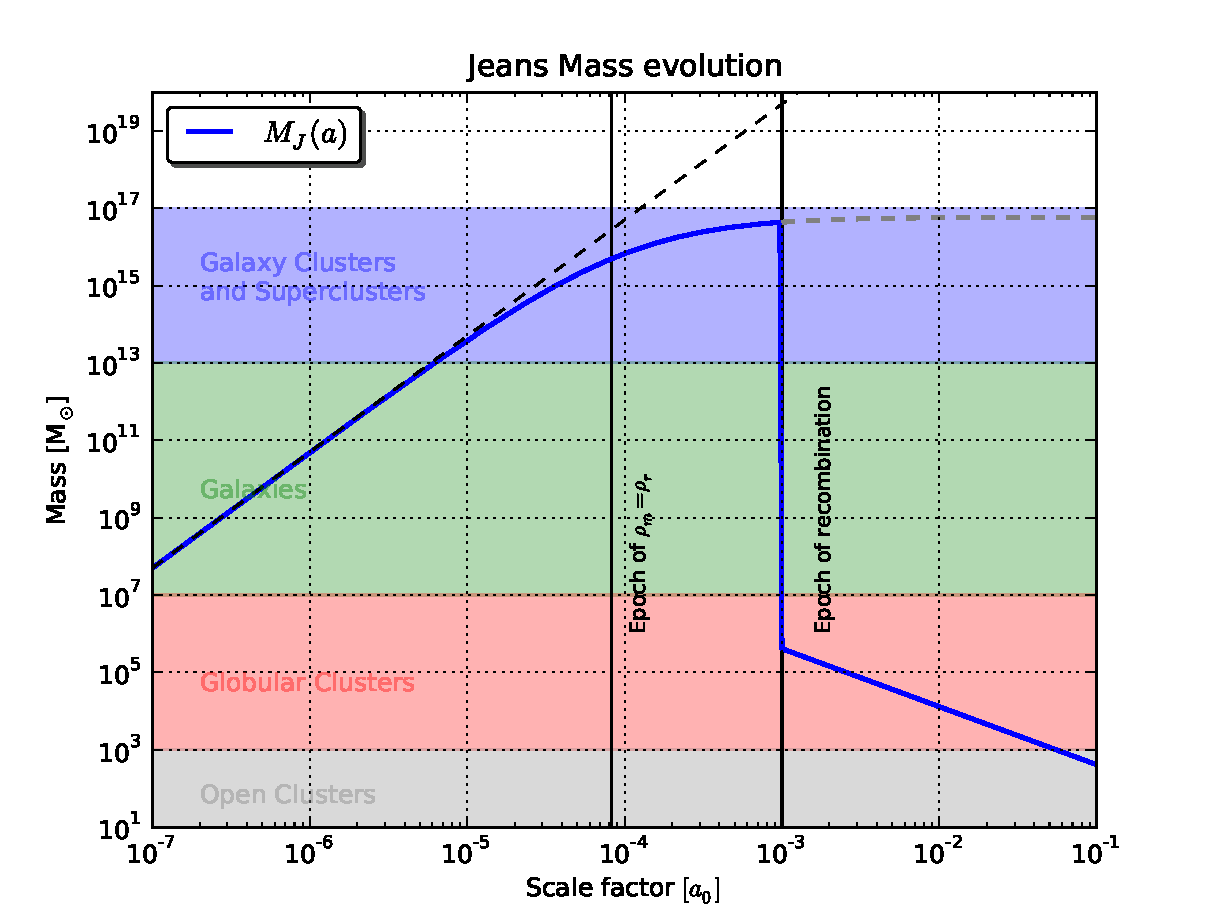
\includegraphics[width=0.9\textwidth]
	{./figures/2_theoretical_framework/Jeans_Mass_Evolution.pdf}

	\caption{\small{Evolution of the Jean mass for different stages of the
	universe. Coloured regions illustrate the typical mass range of some 
	types of structures, since open stellar clusters to superclusters of 
	galaxies.}}
	
	\label{fig:JeansMass}
\end{figure}
%.........................................................................	
	

%Reviewed
The previous analysis has allowed to establish the minimal mass of a 
perturbation in order to collapse. Next it is studied the evolution of 
such perturbations in expanding mediums. For this it is used the models of 
the universe derived in the subsection 
\ref{subsec:SimpleSolutionsOfTheUniverse} and the general equation 
\ref{eq:ContinuityEquationCMode} for evolving perturbations.



%.........................................................................
%Solutions to Perturbations Evolution
\begin{itemize}
\item \textbf{Einstein - de Sitter universe}


%Reviewed
Bearing in mind that for this type of universe $\Omega_m = \Omega_0 = 1$, 
using the Hubble's function \ref{eq:EinsteindeSitter}, the solution for 
the scale factor \ref{eq:EinsteindeSitterSolution}, the velocity of sound 
derived from \ref{eq:SoundVelocity} and the equation of state for an ideal 
gas, it leads to the below expression for the evolution of the 
perturbations


%Reviewed
%.........................................................................	
%Einsten-de Sitter Perturbations
\eq{eq:EinstendeSitterPerturbations}
{ \delta_{\bds k}(a) = \delta_{\bds k, 0} \pr{\frac{a}{a_{\submath{ref}}}}^{1} }
%.........................................................................
where $\delta_{\bds k, 0}$ are the conditions of the field over the 
reference time $t_{\submath{ref}}$. Another possible solution is 
$\delta_{\bds k}\propto a^{-3/2}$, but because this solution does not 
decrease over time, it is not interesting.



%Radiation Dominated Universe
\item \textbf{Radiation-dominated universe}


%Reviewed
For perturbations in a radiation-dominated universe with $\Omega_r = 
\Omega_0 = 1$, using the equation \ref{eq:RadiationUniverseSolution}, it
is obtained


%Reviewed
%.........................................................................	
%Radiation Perturbations
\eq{eq:RadiationPerturbations}
{ \delta_{\bds k}(a) = \delta_{\bds k, 0} \pr{\frac{a}{a_{\submath{ref}}}}^{1.22} }
%.........................................................................
where $\delta_{\bds k, 0}$ again represents  the initial modes of the 
field, divergent solutions are ignored.



%Vacuum Dominated Universe
\item \textbf{Vacuum-dominated universe}
			

%Reviewed
For a universe with cosmological constant $\Omega_\Lambda$
\footnote{$\Omega_\Lambda < 1 $ in order to guarantee the convergence of 
solutions to the Friedmann's equation (see subsection 
\ref{subsec:SimpleSolutionsOfTheUniverse}).} it is obtained the next 
behaviour for the evolution of each mode



%.........................................................................	
%Vacuum Perturbations
\eq{eq:VacuumPerturbations}
{ \delta_{\bds k}(a) = \delta_{\bds k, 0} \pr{\frac{a}{a_{\submath{ref}}}}^{0.58} }
%.........................................................................
\end{itemize}
%.........................................................................


%Reviewed
Plotting each one of these solutions, Figure \ref{fig:DeltaEvolution} is 
obtained. For simplicity and in order to illustrate in a better way the 
behaviour of the scale factor, it is normalized each solution with respect
to their respective value in the reference time $\delta_{\bds k, 0}$.


%Reviewed
Initial conditions depend on the comoving wavenumber $\bds k$ and must be
determined from the statistical properties of the density field (see 
subsection \ref{subsec:StatisticalProperties}) and observational 
measurements, for instance the cosmic background radiation.



\newpage


%Reviewed
%.........................................................................
%Perturbations Evolution
\begin{figure}[htbp]
	\centering
	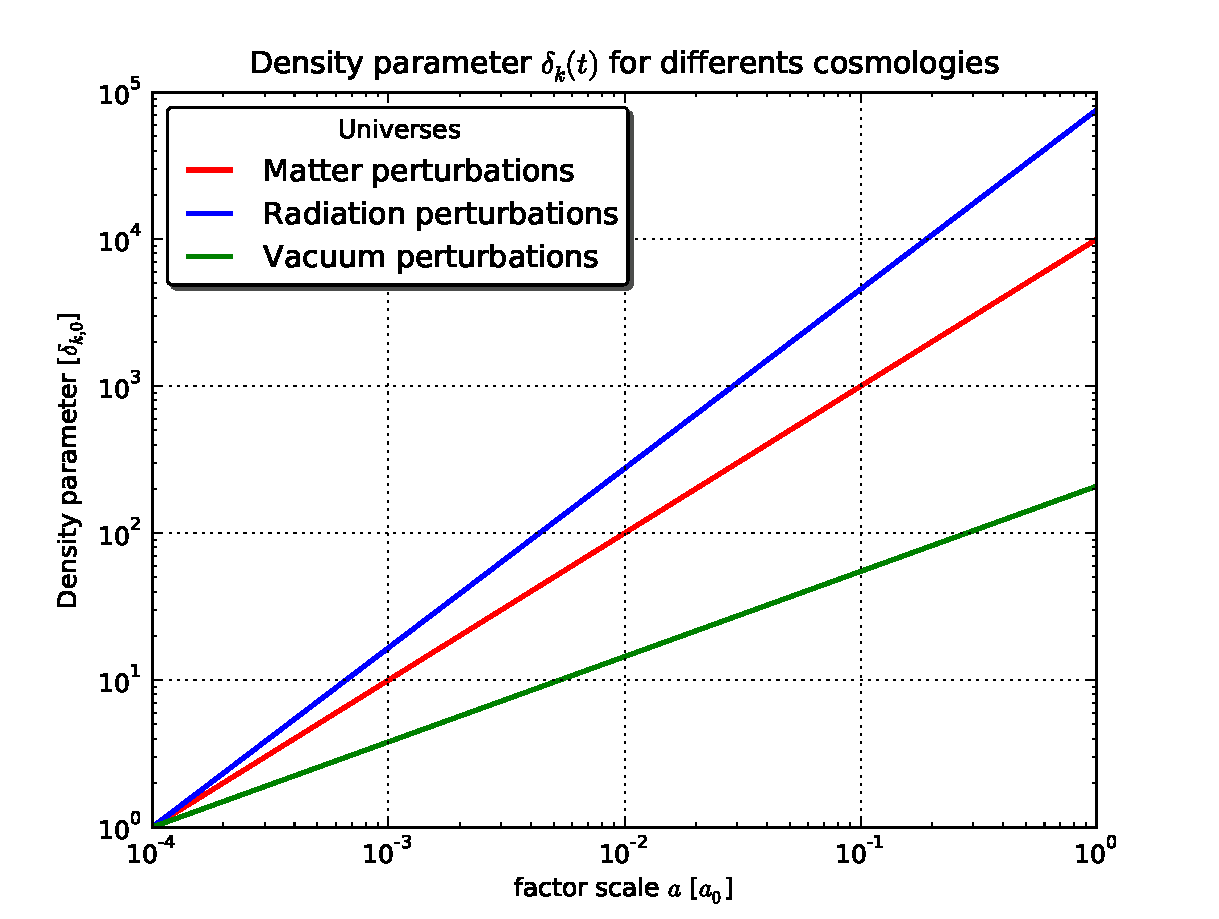
\includegraphics[width=0.9\textwidth]
	{./figures/2_theoretical_framework/Perturbations_Evolution.pdf}

	\caption{\small{Evolution of the normal modes of the density field.
	For the sake of the illustration, each solution has been normalized
	with respect to the initial conditions.}}
	
	\label{fig:DeltaEvolution}
\end{figure}
%.........................................................................	



	%---------------------------------------------------------------------
	%Statistical Properties and Transfer function
	\subsection{Propiedades Estadísticas y Función de Transferencia}
	\label{subsec:StatisticalProperties}
	%---------------------------------------------------------------------



Una vez determinada la evolución de los modos de densidad es necesario 
compararlos con el universo real. Debido a la naturaleza continua de 
los campos es inviable tratar de determinar de forma ob\-servacional la 
distribución de densidad, más aún, teniendo en cuenta que la mayor parte de 
la materia es oscura, la cual solo puede ser inferida de forma indirecta,
resulta también técnicamente imposible con los instrumentos actuales llevar 
a cabo esta empresa.


A pesar de lo anterior es posible aún medir las propiedades estadísticas
de la distribución de densidad del universo y comparar con lo obtenido de
forma teórica. Para esto se introduce el concepto de funcional de 
probabilidad para un campo continuo $P\cor{ \delta(\bds r,t) }$, definido 
como la probabilidad de que un cierto campo físico tenga la forma funcional 
específica $\delta(\bds r,t)$.


Una manera más conveniente, en términos computacionales, de aplicar el 
formalismo de funcional de probabilidad se logra discretizando el espacio 
en celdas de volumen $\Delta^3 \bds r_i$, de tal forma que una cierta 
forma funcional del campo de densidad $\delta(\bds r,t)$ sea equivalente a 
tener simultáneamente en cada celda $\bds r_i$ del grid el valor 
$\delta_i = \delta(\bds r_i)$, así el funcional de probabilidad se 
transforma en una función de probabilidad conjunta


%.........................................................................
%Probability Functional
\eq{eq:ProbabilityFunctional}
{ P\cor{ \delta(\bds r,t)} \ \ \longrightarrow \ \ 
\mathcal{P}_{\bds{r}}(\delta_1,\delta_2,\cdots,\delta_N;t)  }
%.........................................................................


Teniendo en cuenta la descomposición de Fourier del campo de densidad 
$\delta(\bds r,t)$ en las ecuaciones \ref{eq:FourierFields}, es posible 
definir una función de probabilidad conjunta en el espacio recíproco 
$\mathcal{P}_{\bds k}(\delta_{\bds k_1},\delta_{\bds k_2}, \cdots,
\delta_{\bds k_N};t)$ que caracteriza completamente la probabilidad de 
una distribución específica $\delta_{\bds k}(t)$.


La principal motivación de trabajar en el espacio recíproco de debe a que
es posible usar la aproximación de modos incorrelacionados en la cual se
asume que cada modo evoluciona de forma independiente. En el espacio real 
no es posible realizar esto debido a que el largo alcance de la interacción
gravitacional acopla fuertemente el campo densidad entre diferentes 
lugares. Una consecuencia directa de la anterior aproximación es expresar 
la función de probabilidad conjunta como el producto de $N$ distribuciones
individuales \cite{padmanabhan1995}


%.........................................................................
%Probability Functional Recipro
\eq{eq:ProbabilityJointFour}
{ \mathcal{P}_{\bds k}(\delta_{\bds k_1},\delta_{\bds k_2},
\cdots,\delta_{\bds k_N};t) = \prod_{\bds k_i}g_{\bds k_i}( \delta_{\bds k_i};t )  }
%.........................................................................
donde 


%.........................................................................
%Inverse Fourier Delta
\eq{eq:InverseFourierDelta}
{ \delta_{\bds k} = 
\int_V \delta(\bds r) e^{-i \bds k \cdot \bds r} d^3 \bds r  }
%.........................................................................
$g_{\bds k_i}$ la distribución individual de cada modo, $V=L^3$ el volumen 
de normalización y $\bds k = (2\pi/L)\bds n$, con $\bds n$ un vector de 
componentes enteras que caracterizan el modo específico.


Asumiendo que las perturbaciones primordiales del campo de densidad se 
ori\-ginaron por el proceso de inflación cósmica, es posible demostrar que 
la distribución de los modos normales $g_{\bds k_i}$ es una función 
Gaussiana \cite{padmanabhan1995}. Por conveniencia se descompone en 
coordenadas polares complejas el modo de densidad $\delta_{\bds k} = 
r_{\bds k}\exp\pr{ i \phi_{\bds k} }$, obteniendo la siguiente distribución


%.........................................................................
%Gaussian Distribution
\eq{eq:GaussianDistribution}
{ g_{\bds k}( r_{\bds k}, \phi_{\bds k}; t ) = 
\frac{2(r_{\bds k} dr_{\bds k})}{\sigma_k^2}\pr{ \frac{d\phi_{\bds k}}{2\pi} }
\exp\pr{ -\frac{r_{\bds k}^2}{\sigma_k^2} };\ \ \ \ \ \sigma_k^2 = 2\mu_k^2  }
%.........................................................................
donde $\mu_k^2$ es la varianza de la distribución y $\sigma_k^2$ se 
denomina espectro de potencia. Debido a la asunción de isotropía y 
homogeneidad para el universo de fondo, ambas cantidades solo dependen de 
la magnitud del vector de onda $|\bds k| = k$. También es directo mostrar 
las siguientes propiedades de la distribución del campo


%.........................................................................
%Distribution Properties
\eq{eq:Distribution Properties}
{ \bra \delta_{\bds k} \ket = 0;\ \ \ \ \ 
  \bra |\delta_{\bds k}|^2 \ket = \sigma_k^2;\ \ \ \ \ 
  \bra \delta_{\bds k} \delta_{\bds p}\ket = 0\ \ \ \mbox{si}\ \ \ \
  \bds k \neq \bds p }
%.........................................................................


%.........................................................................
%Initial density
\begin{figure}[htbp]
	\centering
	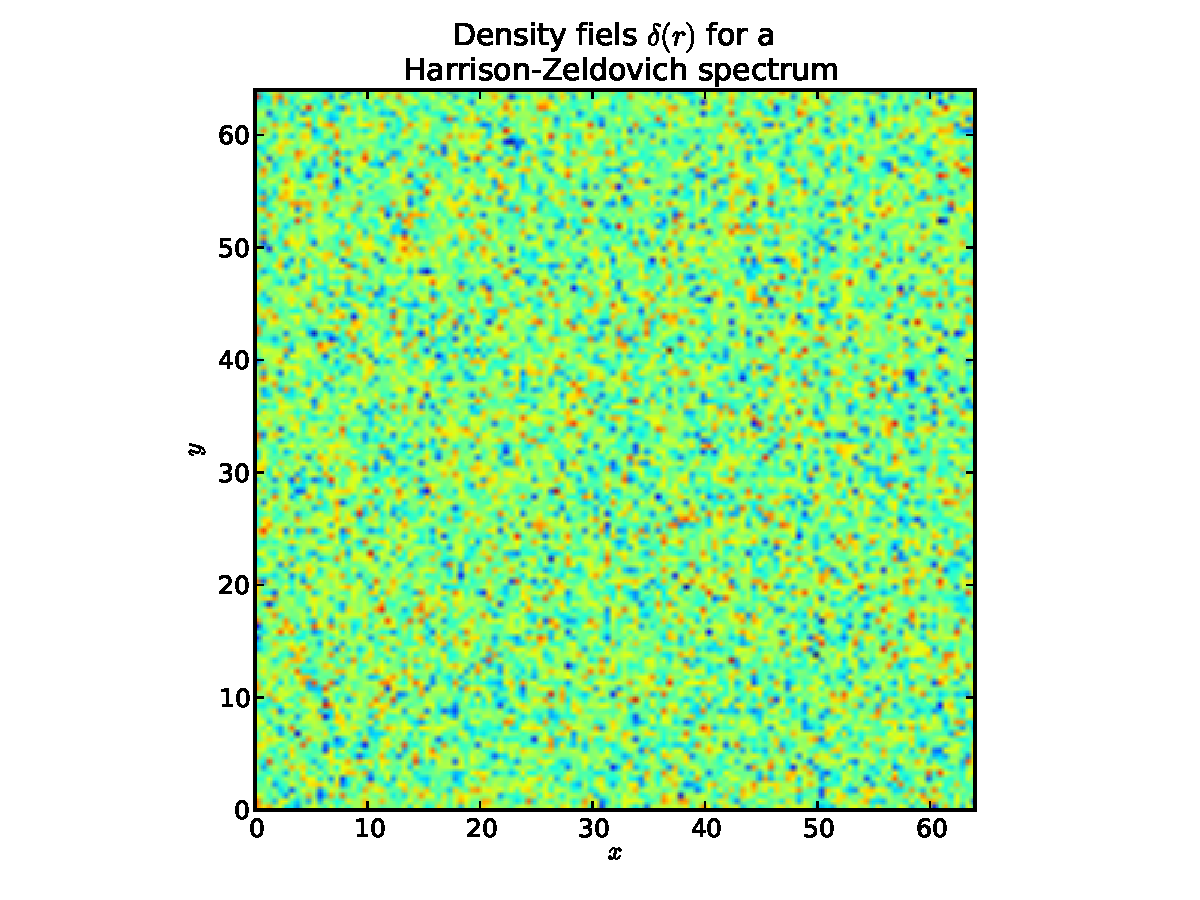
\includegraphics[width=0.9\textwidth]
	{./figures/2_theoretical_framework/Initial_Density.pdf}

	\caption{\small{Distribución inicial de perturbaciones para el campo
	de contraste de densidad a partir de la distribución Gaussiana 
	\ref{eq:GaussianDistribution} y el espectro de potencia de Harrison-
	Zeldovich $\sigma_k \propto k$.}}
	
	\label{fig:InitialDensity}
\end{figure}
%.........................................................................	


Una cantidad que puede ser evaluada directamente es la función de 
correlación de dos puntos $\xi(\bds r) \equiv \bra \delta(\bds r' + \bds r)
\delta(\bds r') \ket$, definida como la probabilidad de tener una 
perturbación a una distancia $\bds r$ de otra. Es una medida directa del 
grado de anisotropía y las propiedades de clustering de una distribución.


%.........................................................................
%Two Points Correlation Function
\begin{eqnarray}
\nonumber
\xi(\bds r) = \bra \delta(\bds r' + \bds r) \delta(\bds r') \ket &=& 
\frac{1}{V^2}\sum_{\bds k, \bds p} \bra \delta_{\bds k} \delta_{\bds p}^*\ket
\exp\cor{ i\bds k \cdot(\bds r' + \bds r)- i\bds p \cdot \bds r' } \\
\label{eq:2PCorrelation}
&=& \int \frac{V^{-1}}{(2\pi)^3}\sigma_k^2 e^{i \bds k \cdot \bds r} d^3 \bds k
\end{eqnarray}
%.........................................................................
donde en la última línea se ha realizado el límite al continuo. La 
expresión \ref{eq:2PCorrelation} muestra que $\sigma_k^2$ es la 
transformada de Fourier de la función de correlación, es decir


%.........................................................................
%Two Points Correlation Function Fourier
\eq{eq:2PCorrelationF}
{ V^{-1}\sigma_k^2 = \int \xi(\bds r) e^{-i\bds k\cdot \bds r}d^3 \bds r }
%.........................................................................


La anterior relación junto con la distribución Gaussiana del campo muestra 
que tanto el espectro de potencia como la función de correlación contienen
toda la información estadística del campo de densidad en el régimen lineal.
En caso de asumir una distribución no-Gaussiana es necesario tener más
momentos de la distribución, tal como la función de correlación de tres 
puntos, etc.


			%-------------------------------------------------------------
			%Harrison-Zeldovich Power Spectrum
			\subsubsection*{Espectro de potencia de Harrison-Zeldovich}
			%-------------------------------------------------------------
			

Una primera aproximación al espectro de potencia, y que puede ser 
demostrada con el modelo de inflación cósmica para las perturbaciones 
primigenias \cite{padmanabhan1995}, es una ley de potencia de la forma


%.........................................................................
%Power Spectrum power
\eq{eq:PowerSpectrumPower}
{ \sigma_k^2 = A k^{n_s} }
%.........................................................................
donde $A$ es un factor de normalización y $n$ es el índice espectral. En 
el caso específico en que $n_s=1$ se denomina espectro de potencia de 
Harrison-Zeldovich y es invariante de escala \footnote{El valor determinado 
observacionalmente es muy cercano $n_s = 0.963$ (ver tabla
\ref{tab:CosmologicalParameters}).}.


Para determinar el factor de normalización es común aplicar un filtro a 
los modos normales que contribuyen al campo de densidad, con esto la 
función de correlación queda


%.........................................................................
%Two Points Correlation Function Fourier with Filter
\eq{eq:Filter2PCorrelation}
{ \xi(\bds r;R) = \int \frac{V^{-1}}{(2\pi)^3}\sigma_k^2 
e^{i \bds k \cdot \bds r} \tilde{W}(k;R) d^3\bds k }
%.........................................................................
donde $R$ determina la escala máxima a partir de la cual se aplica el 
filtro en los modos del campo y $\tilde{W}(k;R)$ es la transformada de
Fourier de la función de filtro. En especial se define la dispersión en el
espacio real asociada a una escala $R$ como $\sigma^2_R = \bra \delta^2 \ket=
\xi(0; R)$, este parámetro puede ser determinado observacionalmente a partir
de surveys de galaxias y de la radiación cósmica de fondo, en especial el 
valor estándar definido por el WMAP7 es $\sigma^2_8 = \xi(0; R = 
8 \mbox{ Mpc}/h) = 0.801$ (ver tabla \ref{tab:CosmologicalParameters}), con
esto se llega a


%.........................................................................
%Normalization Expression
\eq{eq:Normalization}
{ \sigma_8^2 = A\int \frac{V^{-1}}{(2\pi)^3} k^{n_s}
 \tilde{W}(k;R=8 \mbox{ Mpc}/h) d^3\bds k }
%.........................................................................
de esta forma, a partir de los valores medidos de $n_s$ y $\sigma_8^2$, es
posible encontrar la normalización del espectro de potencia.


			%-------------------------------------------------------------
			%Transfer Function
			\subsubsection*{Función de Transferencia}
			%-------------------------------------------------------------
			

Finalmente para el régimen lineal se introduce el concepto de función de 
trans\-ferencia $T_{\bds k}(t)$, definida a partir de la siguiente 
expresión


%.........................................................................
%Transfer function Definition
\eq{eq:TransferFunction}
{ \delta_{\bds k}(t) = T_{\bds k}(t) \delta_{\bds k}(t_i) }
%.........................................................................
donde $t_i$ es un tiempo de referencia, normalmente la época de 
recombinación en el caso de perturbaciones de materia.


De la expresión \ref{eq:TransferFunction} se infiere que la función de 
transferencia contiene toda la información dinámica de las perturbaciones,
más aún, de la definición \ref{eq:Distribution Properties} para el espectro
de potencia se tiene


%.........................................................................
%Power Spectrum and Transfer Function
\eq{eq:PkTransferFunction}
{ \sigma_k(t) = \sigma_k(t_i)|T_k(t)|^2 = Ak^{n_s} |T_k(t)|^2 }
%.........................................................................
donde se ha asumido un espectro de potencia de Harrison-Zeldovich para el 
tiempo de referencia. Con esto finalmente se concluye que la función de 
transferencia también permite obtener todas las propiedades estadísticas 
del campo durante el tiempo en que el régimen lineal es válido.


El cálculo de la función de transferencia es generalmente complejo y 
requiere realizarse numéricamente \footnote{\texttt{CMBFAST} es un 
software bastante conocido para este propósito 
\url{http://lambda.gsfc.nasa.gov/toolbox/tb_cmbfast_ov.cfm}}, además
depende de las propiedades específicas de la especie asociada a la
perturbación. Como un ejemplo, en el caso de perturbaciones de materia 
oscura debe ser especificado el tipo de partículas que la componen, ya 
sean partículas livianas relativistas (materia oscura caliente) o 
partículas pesadas no relativistas (materia oscura fría). Entre ambos 
casos la función de transferencia y el espectro procesado 
\ref{eq:PkTransferFunction} difieren bastante debido a las diferentes 
ecuaciones de estado asociadas a cada tipo.


En el caso de perturbaciones adiabáticas (isoentrópicas) de materia 
oscura fría puede usarse la siguiente aproximación analítica para la 
época actual \cite{longair2008}


%.........................................................................
%Transfer Function CDM
\eq{eq:TransferFunctionCDM}
{ T_k \approx \frac{ \ln\pr{ 1 + 2.34 q } }{2.34 q}
\cor{ 1 + 3.89 q + \pr{ 1.61 q }^2 + \pr{ 5.46 q }^3 + \pr{ 6.71 q }^4}^{-1/4} }
%.........................................................................
donde $q \equiv k/\Omega_0 h^{2} \mbox{ Mpc}^{-1} $.


En la siguiente figura se ilustra la función de transferencia 
\ref{eq:TransferFunctionCDM} junto con el espectro de potencia procesado

%.........................................................................
%Transfer Function CDM
\begin{figure}[htbp]
	\centering
	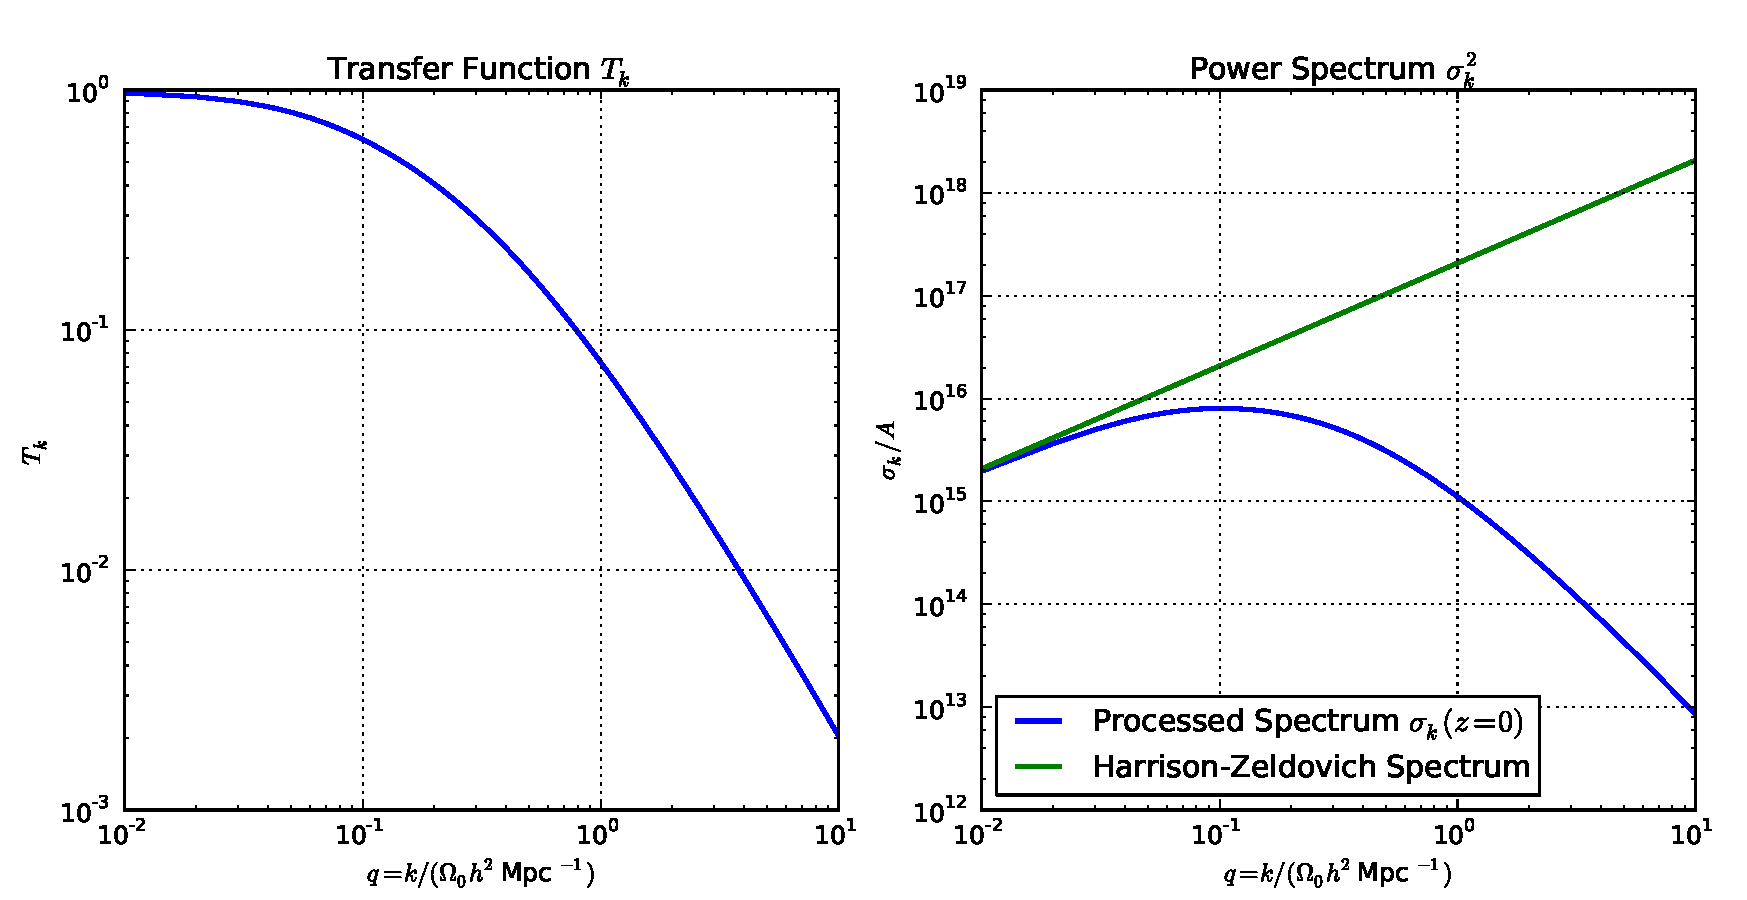
\includegraphics[width=0.9\textwidth]
	{./figures/2_theoretical_framework/Transfer_Function.pdf}

	\caption{\small{Función de transferencia para materia oscura fría en la
	época actual \cite{longair2008} (Izquierda). Comparación entre el 
	espectro de potencia inicial, Harrison-Zeldovich, y el espectro de 
	potencia procesado (derecha).}}
	
	\label{fig:TransferFunctionCDM}
\end{figure}
%.........................................................................	


De todo el formalismo desarrollado en esta sección se concluye que el 
objetivo final para la caracterización del régimen lineal es obtener la 
función de transferencia, ya que esta determina completamente la 
evolución del universo en épocas tempranas donde hay alta homogeneidad e
isotropía en todas las escalas.


%*************************************************************************




%*************************************************************************
%NonLinear Structure Formation
\section{Régimen No Lineal de Formación de Estructuras}
\label{sec:NonLinearStructureFormation}


En el régimen lineal se describe el proceso de formación de estructuras 
como perturbaciones en un universo de fondo homogéneo e isotrópico. Cuando
las perturbaciones crecen tal que $\delta \gtrsim 1$ la autogravedad de 
los modos acopla fuertemente el campo de forma local y e invalida la 
aproximación lineal. Los procesos físicos asociados al régimen no lineal
son altamente complejos e inclusive algunos no son bien entendidos en la 
actualidad, esto hace que solo sea posible abordar satisfactoriamente el 
problema a través de simulaciones numéricas (ver capítulo 
\ref{cha:N-BodySimulations}).


%.........................................................................
%Nonlinear Universe
\begin{figure}[htbp]
	\centering
	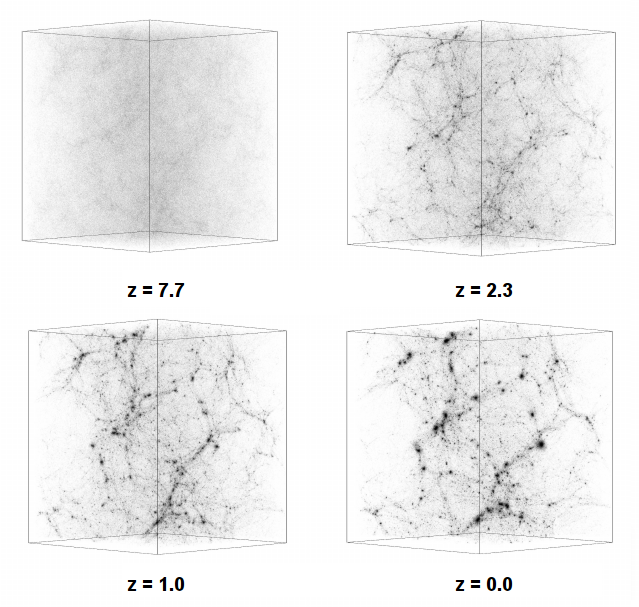
\includegraphics[width=0.9\textwidth]
	{./figures/2_theoretical_framework/Nonlinear.png}

	\caption{\small{Evolución de una simulación numérica de materia oscura
	en una caja de 40 Mpc$/h$, iniciando en un estado de alta homogeneidad 
	(arriba-izquierda) hasta la época actual de estructuras altamente no 
	lineales (abajo-derecha). Tomado de 
	\url{http://www.astro.utu.fi/research/CosmoS/lss/lss_p1.shtml}}}
	
	\label{fig:NonLinearUniverse}
\end{figure}
%.........................................................................


La figura \ref{fig:NonLinearUniverse} corresponde a una simulación 
numérica de materia oscura para el universo en régimen no lineal. En esta 
pueden ser apreciadas algunas propiedades emergentes tales como la 
anisotropía e inhomogeneidad a escalas peque\-ñas ($\sim$ Mpc), la 
formación y clustering de estructuras altamente no lineales y la aparición 
de un patrón de red a grandes escalas (red cósmica).


	%---------------------------------------------------------------------
	%Zeldovich's Approximation
	\subsection{Aproximación de Zeldovich}
	\label{subsec:Zeldovich'sApproximation}
	%---------------------------------------------------------------------
	

A pesar de la complejidad del régimen no lineal, cuando las perturbaciones 
en el campo de densidad aún no son mucho mayores que el valor de fondo 
puede realizarse una desarrollo analítico de la evolución, esto es conocido
como aproxi\-mación de Zeldovich y fue desarrollada en 1970 por Yakov 
Zeldovich en \cite{zeldovich1970}. Para formular esta aproximación es 
conveniente expresar de nuevo el campo de contraste de densidad 
$\delta(\bds r)$ en términos de coordenadas comóviles y no respecto a los 
modos normales de Fourier, esto debido a que en este régimen los modos no 
son independientes y usarlos no simplifica el tratamiento, a diferencia 
del régimen lineal. 


Usando el marco de referencia Lagrangiano de una cierta porción de fluido
o distribución de materia, su trayectoria $\bds r_f$ puede ser descrita 
mediante la siguiente expresión


%.........................................................................
\eq{eq:ZeldovichTrayectory}
{ \bds r_f( t,\bds q ) = a(t)\bds r = a(t)\cor{ \bds q + \bds \Psi(\bds q,t) } }
%.........................................................................
donde $\bds r$ es la posición comóvil de la porción de fluido, $\bds q$ 
su coordenada Lagrangiana inicial cuando el fluido no está perturbado y 
$\bds \Psi(\bds q,t)$ se denomina función de desplazamiento y da cuenta de 
las perturbaciones en el medio. 


A partir de la ecuación de evolución del campo de contraste de densidad 
\ref{eq:DeltaEvolution} es posible demostrar que el campo de desplazamiento 
$\bds \Psi(\bds q,t)$ satisface \cite{Yoshisato2006}


%.........................................................................
%Displacement Differential Equation
\eq{eq:Displacement}
{ \der{^2  \bds \Psi}{t^2} + 2H\der{\bds \Psi}{t} =
 \frac{ 3}{2}H^2 \bds \Psi  }
%.........................................................................
de esto se obtiene finalmente


%.........................................................................
%Displacement Explicit Form
\eq{eq:DisplacementForm}
{ \bds \Psi = \frac{3}{2}H_0^{-2}a(t)\nabla \Phi  }
%.........................................................................
donde $\Phi$ es el potencial gravitacional efectivo asociado al campo de 
densidad por medio de la ecuación de Poisson \ref{eq:PoissonEquationC}.


Expresando la conservación de la masa en términos de las coordenadas 
comóviles y las coordenadas Lagrangianas iniciales, se debe satisfacer


%.........................................................................
%Mass Conservation
\eq{eq:MassConservation}
{ \rho(\bds r, t)d^3 \bds r = \bar{\rho}(t)d^3 \bds q  }
%.........................................................................
calculando ahora el Jacobiano $\partial q_i / \partial r_j$ de la 
transformación $\bds r \rightarrow \bds q$, el campo de densidad perturbado 
pude se escrito como \cite{padmanabhan1995}


%.........................................................................
%Perturbed Field Density
\eq{eq:PerturbedFieldDensity}
{ \rho(\bds r, t) = \frac{\bar \rho (t)}{\pr{ 1 - a(t) \lambda_1(\bds q)}
\pr{ 1 - a(t) \lambda_2(\bds q)}\pr{ 1 - a(t) \lambda_3(\bds q)} } }
%.........................................................................
donde $-\lambda_i(\bds q)$ son los autovalores del Jacobiano y están 
ordenados de tal forma que $\lambda_1\geq\lambda_2\geq\lambda_3$. Cada uno
de estos autovalores pueden ser interpretados de forma geométrica como un 
indicador del colapso o expansión de una porción de fluido en la dirección
correspondiente al autovector respectivo, así por ejemplo si $\lambda_i > 0$,
implica que el campo de densidad está colapsando localmente en la dirección 
del autovector $\bds u_i$, mientras que $\lambda_i < 0$ implica una 
expansión en la misma dirección.

\
%.........................................................................
%Zeldovich Approximation Comparison
\begin{figure}[htbp]
	\centering
	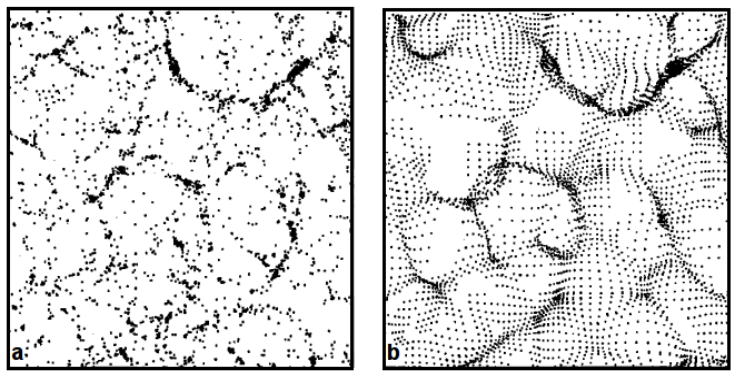
\includegraphics[width=0.9\textwidth]
	{./figures/2_theoretical_framework/Zeldovich_Approximation.png}

	\caption{\small{Comparación de la evolución en régimen no lineal entre
	una simulación de N-cuerpos (a), y la aproximación de Zeldovich (b).
	En ambos casos se usan las mismas condiciones iniciales. Tomado de 
	\cite{longair2008}. }}
	
	\label{fig:ZeldovichComparison}
\end{figure}
%.........................................................................


Finalmente en la figura \ref{fig:ZeldovichComparison} se muestra una 
comparación entre una simulación numérica de N-cuerpos y la aproximación 
de Zeldovich, puede notarse una alta semejanza visual en las estructuras 
obtenidas en los dos casos al final de la evolución, demostrando la alta 
precisión del método. En la sección \ref{sec:EnvironmentCharacterization}
se hace uso de la idea general planteada en la aproximación de Zeldovich 
respecto a los autovalores del Jacobiano de la transformación, para la 
construcción de esquemas de clasificación del entorno cosmológico a partir 
de los autovalores de otras cantidades físicas más adecuadas para la 
descripción de la dinámica local del campo de densidad, tales como el 
tensor de marea o el tensor de velocidad peculiar.


%*************************************************************************	

%--------------------- Nbody simulations ------------------------
%qqqqqqqqqqqqqqqqqqqqqqqqqqqqqqqqqqqqqqqqqqqqqqqqqqqqqqqqqqqqqqqqqqqqqqqqq
%Quote
\begin{savequote}[50mm]
‘‘All the effects of Nature are only the mathematical consequences of a 
small number of immutable laws’’
\qauthor{Pierre Simon Laplace}
\end{savequote}
%qqqqqqqqqqqqqqqqqqqqqqqqqqqqqqqqqqqqqqqqqqqqqqqqqqqqqqqqqqqqqqqqqqqqqqqqq




%#########################################################################
\chapter{Computational Methods in Cosmology}
\label{cha:N-BodySimulations}


%Reviewed
In recent years, computational physics has acquired an important role in
physics, allowing modelling a lot of high-complexity systems without the
necessity of recurring to experiments and/or observations. Among the methods
covered by computational physics is highlighted the N-body problem since 
many phenomenons require the computation of the interactions between a
large number of bodies. Some illustrative examples of this are the 
modelling of molecular systems, plasma physics and specially gravitational
problems in astrophysics. The development of specific methods to solve 
this type of problems precedes the advent of computer systems, even so, 
their development has powered enormously this discipline such that it is
considered a new branch of physics.


%Reviewed
In this chapter will be covered in detail some specific methods for solving
gravitational problems in astrophysics, specially those related with 
simulations of the large-scale universe in the non-linear regime, ranging 
from basic algorithms to compute forces, methods to detect dark halos, to
basic classification schemes for the cosmological environment.

 

%#########################################################################




%*************************************************************************
%N-body Simulations
\section{N-body Simulations}
\label{sec:N-bodySimulations}


%Reviewed
Generally, the most suitable type of phenomena that can be modelled through 
N-body simulations is those where the interactions are strongly correlated 
between the constituent particles, such as long-range forces or non-local 
interactions. Figure \ref{fig:NbodyProblem} illustrates an arbitrary set 
of point particles which interact each other under the influence of a 
force field $\bds f$. Those conditions shape the classical formulation of 
the N-body problem.


\
%Reviewed
%.........................................................................
%N-Body Problem
\begin{figure}[htbp]
	\centering
	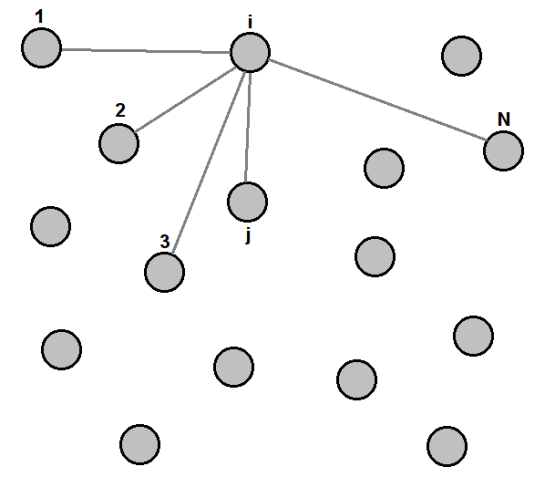
\includegraphics[width=0.50\textwidth]
	{./figures/3_nbody_simulations/Nbody_Problem.png}

	\caption{\small{Formulation of the N-body problem.}}
	
	\label{fig:NbodyProblem}
\end{figure}
%.........................................................................


%Reviewed
Assuming interactions that depends on the position\footnote{ In the 
generalized problem, interactions can depend on other parameters like 
the velocity or intrinsic degrees of freedom like the spin.}, it is 
obtained the below equation of movement of the $i$-th particle shown in 
the Figure \ref{fig:NbodyProblem} \cite{pfalzner1996} \cite{binney2008} 


%Reviewed
%.........................................................................
%Movement Equation
\eq{eq:MovementEquation}
{ \ddot{ \bds r}_i = \sum_{j=1}^N \bds f( \bds r_i, \bds r_j ) = -\nabla 
\phi( \bds r_i )\ \ \ \ \ \ \ i=1,2,\cdots,N }
%.........................................................................
where it has been introduced the potential function $\Phi(\bds r)$. For
the case of gravitational interactions, the potential acquires the form



%.........................................................................
%Gravitational Potential
\eq{eq:GravitationalPotential}
{ \phi(\bds r) = -\sum_{j=1}^N  \frac{G m_j}{|\bds r - \bds r_j|} }
%.........................................................................


%Reviewed
The general solution to the problem is obtained from the set $\{ \bds 
r_1(t),\cdots, \bds r_N(t) \}$, which is determined from the equations
\ref{eq:MovementEquation}. For this it is necessary to implement numerical
approximations due to the non-solvable (analytically) nature of the 
problem.



	%---------------------------------------------------------------------
	%Direct sum
	\subsection{P-P Method}
	\label{subsec:PPMethod}
	%---------------------------------------------------------------------
	
	
%Reviewed
The first approximation to find a solution of the equations of movement
\ref{eq:MovementEquation} is to compute all the $N-1$ interactions of the
$i$-th particle with all of the others in a specific time $t$ and this for
$i=1,2,\cdots N$, then, from a numerical integration scheme it is 
calculated the positions in a discretized later time $t+\Delta t$ and thus
until a given maximum time $t_{\submath{max}}$. This method is called P-P 
(Particle to Particle) and is one of the three standard methods for 
solving the N-body problem.


%Reviewed
When interactions present singularities, such as Coulombic potentials in
electrostatic and gravitational problems (equation 
\ref{eq:GravitationalPotential}), the integration of the equation of 
movement is very sensitive to close encounters between particles and 
therefore the resolution of the time step must be increased, thereby 
implying a considerable increasing of the computing time. A standard 
solution is to introduce a softening parameter that removes these 
singularities, but at the cost of losing accuracy in the solution. For the
gravitational potential \ref{eq:GravitationalPotential}, this leads to


%Reviewed
%.........................................................................
%Gravitational Potential
\eq{eq:SoftPotential}
{ \phi_{s}(\bds r) = -\sum_{j=1}^N  \frac{G m_j}{|\bds r - \bds r_j| 
+ \epsilon_j^2} }
%.........................................................................
where $\epsilon_j$ is the softening parameter and can be interpreted as a
measure of the physical dimension of the particle.


%Reviewed
In spite of the high precision achieved by this method, the computing time
scales as $t_{\submath{comp}}\propto N^2$, what makes it highly non-viable
to apply for a large number of particles (generally $N\gtrsim 10^4-10^5$ 
\cite{padmanabhan1995}). For simulations of planetary systems, computation
of orbits of minor bodies and studies of star clusters dynamics, this 
methods is good enough, but for cosmology and galaxy astrophysics, where 
the number of implicated particles must be the maximum possible in order 
to reproduce the real continuous nature of the matter distribution, it 
becomes necessary to develop methods lesser computational 
cost.



	%---------------------------------------------------------------------
	%Tree codes
	\subsection{PM Method}
	\label{subsec:PMMethod}
	%---------------------------------------------------------------------
	
	
%Reviewed
A second scheme used for solving the N-body problem is the PM scheme 
(Particle Mesh) \cite{dawson1983}, this consists of determining a 
continuous distribution for the density field from the position and the
mass value of each particle, for this it is divided the space of the 
simulation into a grid of $M\times M\times M$ cells and then a count of
particles per cell is made in order to associate a specific mass value and
therefore a density to each cell. An illustrative diagram is shown in 
Figure \ref{fig:MP_Method}


%Reviewed
%.........................................................................
%PM Method
\begin{figure}[htbp]
	\centering
	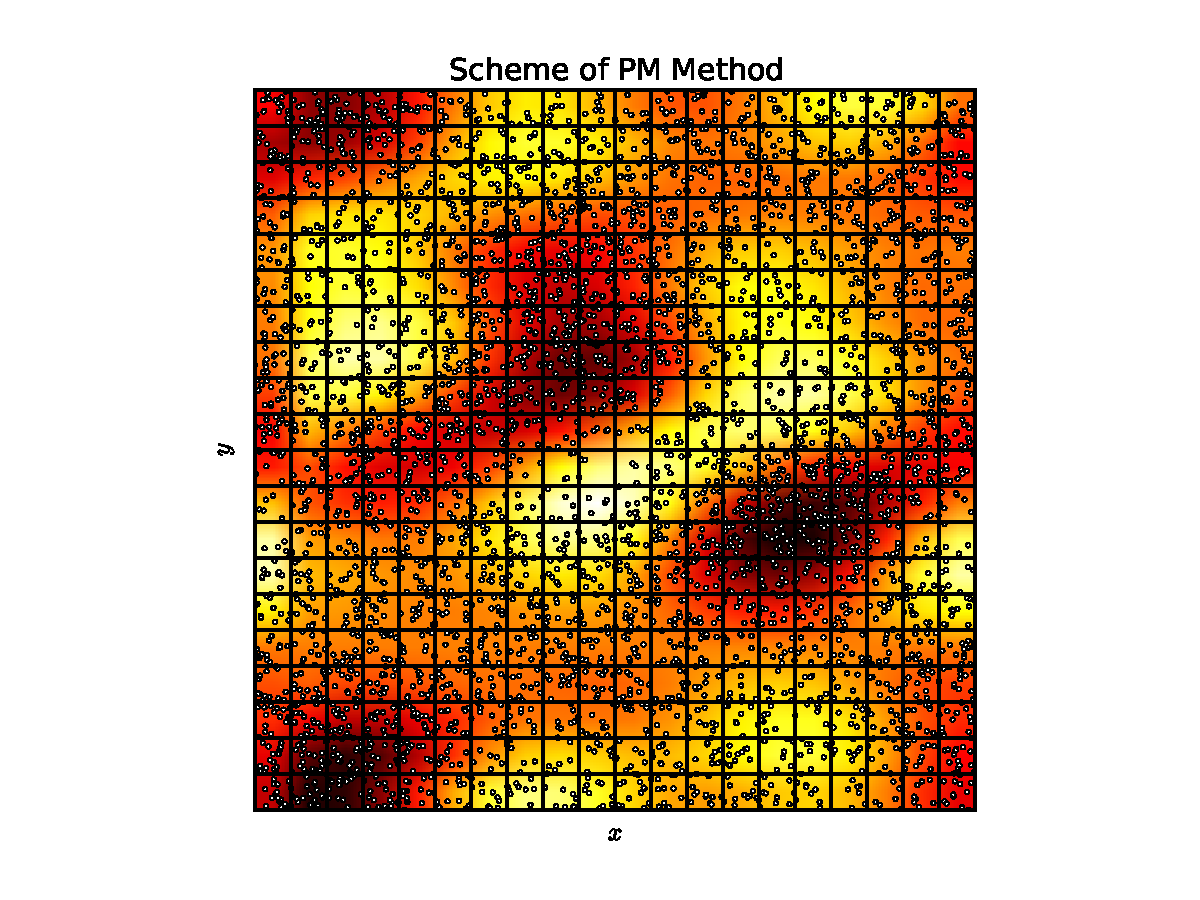
\includegraphics[width=1.00\textwidth]
	{./figures/3_nbody_simulations/PM_Method.pdf}

	\caption{\small{Illustrative diagram of the PM method. The map that is
	plotted over the distribution of particles corresponds to the density
	field evaluated in each cell of the grid. Dark cells corresponds to
	overdensity regions whereas white cells to lower values of the density 
	field, which agrees with the amount of mass of the particles per cell.}}
	
	\label{fig:MP_Method}
\end{figure}
%.........................................................................
%Reviewed
\newpage
The method can be summarized into the next steps


%Reviewed
%.........................................................................
%Particle Mesh steps
\begin{itemize}
\item[\textbf{1.}] From the grid established over all the simulation, it
is calculated a continuous density field $\rho(\bds r)$, interpolating the
value between adjacent cells.

%Reviewed
\item[\textbf{2.}] Once it is obtained the density field, it is calculated
the potential of the equation of movement \ref{eq:MovementEquation} by 
using the Poisson's equation



%.........................................................................
%Poisson Equation
\eq{eq:Poisson}
{ \nabla^2 \phi = 4 \pi G \rho }
%.........................................................................


%Reviewed
In order to reach this, it is usually used integration schemes based upon
Fourier transform, such as the Fast Fourier Transform (FFT).


%Reviewed
\item[\textbf{3.}] Finally, using the previous potential field, it is 
calculated the position of each particle in the next discrete time
$t+\Delta t$, and it is repeated over and over again until a given
final time.
\end{itemize}
%.........................................................................


%Reviewed
This method is less precise than the direct sum, but it is possible to 
demonstrate that the computing time scales as $t_{\submath{comp}} 
\propto N + M \log M$, with an asymptotic behaviour as $t_{\submath{comp}} 
\propto N$ for high resolutions $M$ of the grid and as $t_{\submath{comp}} 
\propto N$ for low resolutions \cite{pfalzner1996}. In any case, its 
efficiency is much better than the PP method \ref{subsec:PPMethod} when
the number of particles of the simulation is large enough $N\ll 10^4 - 
10^5$, which makes this method very useful to tackle problems with a large
number of particles.


%Reviewed
However, there are some pathological situations where this method can not
be applied satisfactory \cite{pfalzner1996}.


%Reviewed
%.........................................................................
%Difficulties of PM Method
\begin{itemize}
\item Highly non-homogeneous distributions of particles.
\item Strongly correlated systems.
\item Systems with non-trivial geometries.
\end{itemize}
%.........................................................................


%Reviewed
Because those conditions are satisfied in the non-linear universe, like 
strong gravitational couplings for modes of the density field after 
$z\gtrsim 8$, this methods is not very useful for solving the late 
universe.



	%---------------------------------------------------------------------
	%Hidrodynamical and dark matter simulations
	\subsection{P$^3$M Method}
	\label{subsec:P3Method}
	%---------------------------------------------------------------------
	
	
%Reviewed
The last of the three standard scheme for solving N-body simulations is 
the P$^3$M method (PP $+$ PM) \cite{hockney1988}. This method can be 
thought as a combination of the previous methods, making the most of each
one of them.


%Reviewed
%.........................................................................
%P3M Method
\begin{figure}[htbp]
	\centering
	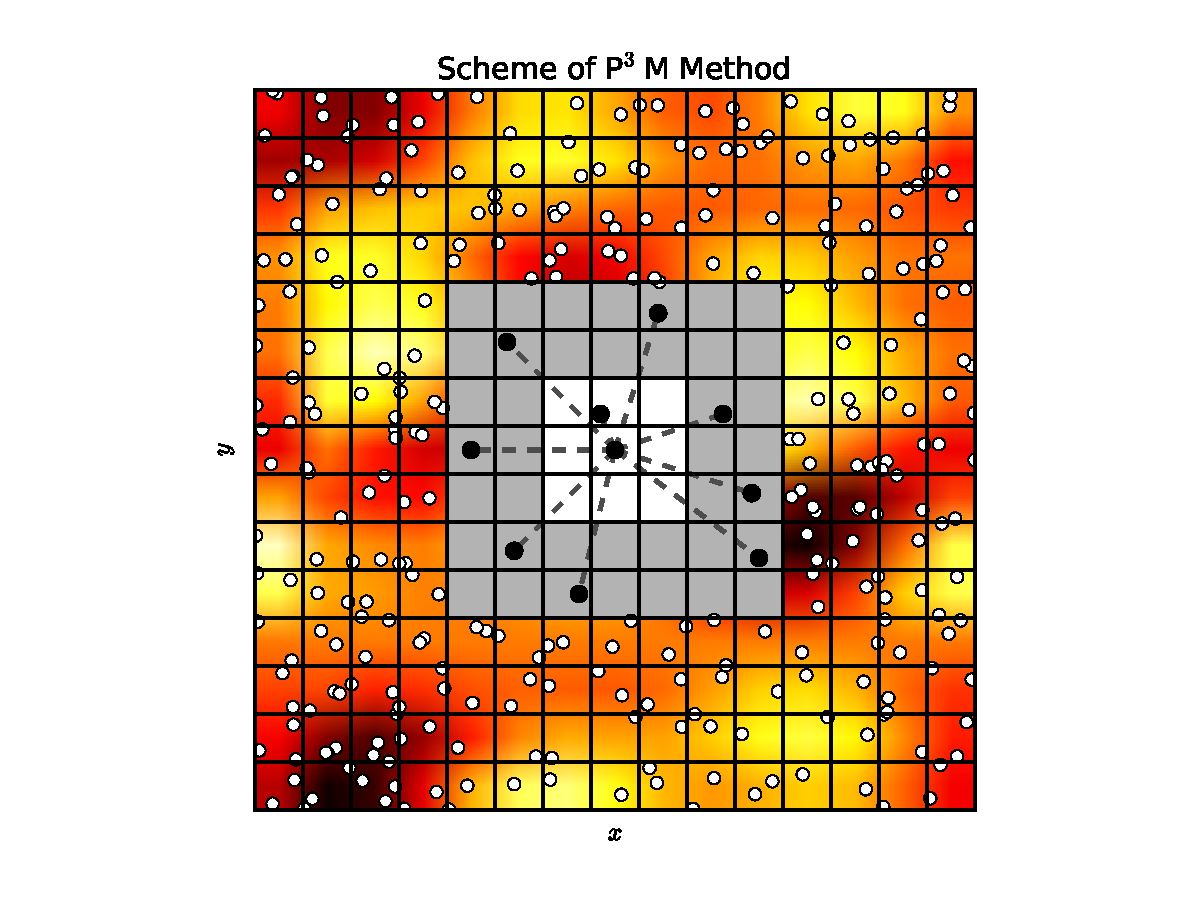
\includegraphics[width=1.00\textwidth]
	{./figures/3_nbody_simulations/P3M_Method.pdf}

	\caption{\small{Illustrative diagram of the P$^3$M method. For the 
	reference particle, shown in the center, interactions with distant 
	particles is calculated through the PM method, whereas for close
	particles (gray and white regions), the interaction is calculated 
	by using the PP method.}}
	
	\label{fig:P3M_Method}
\end{figure}
%.........................................................................


%Reviewed
Figure \ref{fig:P3M_Method} illustrates the P$^3$M method. For each one of
the integration step of the system, it is calculated a hierarchical grid 
for each particle. Hierarchies are defined with respect to the relative
distance between particles and they determines which approximation should
be used for computing the equation of movement. For close particles (first
hierarchy) it is used the PP method, what allows tackling strong local 
correlations and highly non-homogeneous regions. Interactions with 
particles embedded into the next hierarchies are calculated by decomposing 
the potential field into its multipolar terms, i.e. the second hierarchy
corresponds to the dipolar contribution of the potential (if applicable), 
and so on. Finally for more distant cells (last hierarchy), it is used the
PM scheme, interpolating the density field and solving the Poisson's 
equation \ref{eq:Poisson} for the potential.


%Reviewed
%.........................................................................
%Tree Code Building
\begin{figure}[htbp]
	\centering
	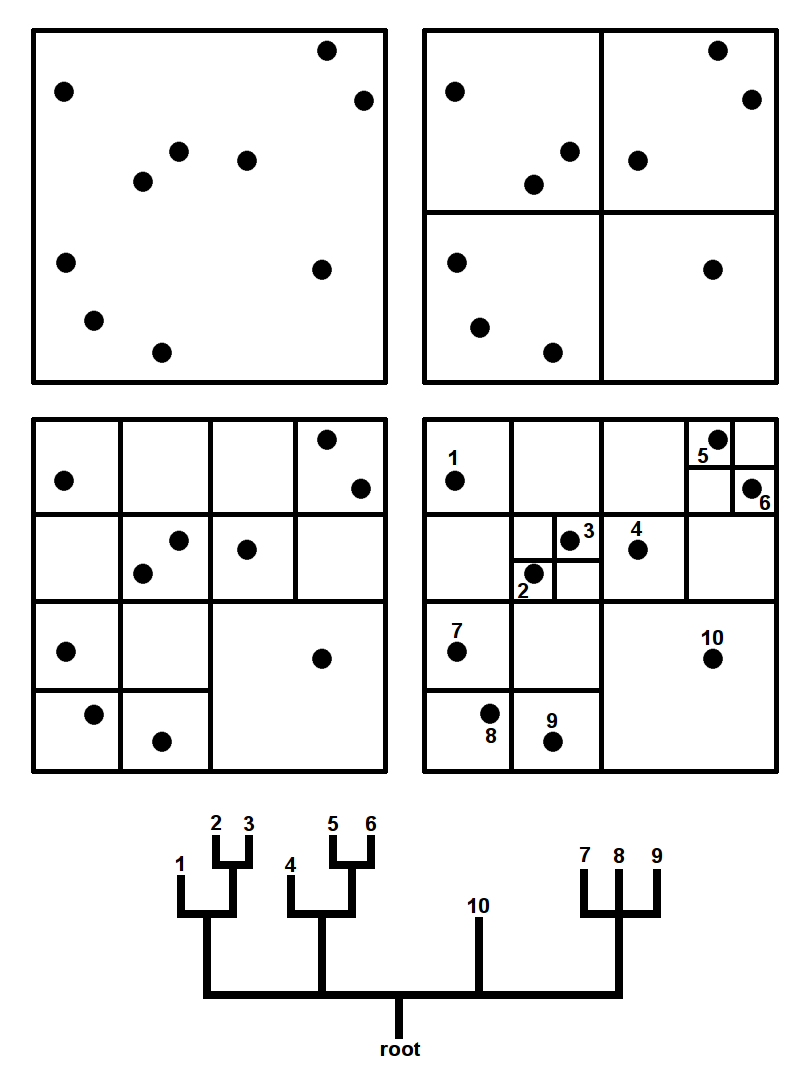
\includegraphics[width=0.72\textwidth]
	{./figures/3_nbody_simulations/TreeCode.png}

	\caption{\small{An illustrative example of the building of a tree code
	for a N-body simulation. Upper panels show the iterations for a 2D 
	problem whereas lower panel illustrates the resultant tree built using 
	each particle of the simulation.}}
	
	\label{fig:Tree_Code}
\end{figure}
%.........................................................................
\newpage


%Reviewed
One of the main disadvantages of this method lies in the building of the
hierarchical structure for evaluating which scheme must be used. The 
original scheme proposed simultaneously by \cite{appel1985} 
\cite{jernigan1985} and \cite{porter1985} has some inconsistencies 
produced by the lack of physical basis in the building of the hierarchical
structure \cite{pfalzner1996}.


%Reviewed
A better physically based method for constructing the hierarchical 
structure of a N-body simulation is the so-called octant tree code. It was
initially developed by \cite{barnes1986}. In this algorithm, the space of 
the simulation is embedded into a cubic volume denominated \textit{root},
then this volume is divided into 8 regions of equal size which are 
denominated octant, these are the first hierarchy of the tree. This 
procedure is repeated recursively until each cell or octant has only one
particle inside, thereby constructing a set of hierarchies that determines
the neighbourhood of all the particles of the simulation. Figure 
\ref{fig:Tree_Code} illustrates the iterations needed in order to construct
the tree of a simulation (with the aim of simplicity, it is 2D), the lower
panel of the same figure shows the structure of the tree. In this way it
is possible to compute, for instance, the interaction between particles 7,
8 and 9 by using direct sum, because they are the closer neighbours, 
whereas the interaction with other particles that belong to other branches
is calculated through the PM scheme.



%*************************************************************************




%*************************************************************************
%Types of simulations
\section{Tipos de Simulación}
\label{sec:Types of Simulations}


Usando los métodos descritos en la anterior subsección es posible realizar
simulaciones del universo en régimen no lineal y estudiar su comportamiento 
de forma numérica. Debido a que en régimen no lineal los procesos 
astrofísicos de grandes escalas son dominados principalmente por materia 
oscura, es habitual no consi\-derar la contribución de las componentes de 
radiación y materia bariónica, además de que los procesos físicos que 
involucran estás componentes aumentarían conside\-rablemente los tiempos 
de cómputo. Este tipo de simulaciones son denominadas \textit{simulaciones 
de materia oscura}.


En esta subsección son presentadas las simulaciones de materia oscura que 
son usadas, además son clasificadas acorde al criterio adoptado para la 
elección de las condiciones iniciales. Estas pueden ser no restringidas
cuando las condiciones iniciales son escogidas de forma completamente 
aleatoria, o restringidas cuando son escogidas de tal forma que la 
simulación satisfaga alguna condición impuesta a priori, tal como la 
reproducción del universo local en una escala de algunas decenas de 
Mpc$/h$.


	%---------------------------------------------------------------------
	%Unconstrained simulations (Bolshoi)
	\subsection{Simulaciones No Restringidas (Bolshoi)}
	\label{subsec:UnconstrainedSimulations}
	%---------------------------------------------------------------------


Puesto que la evolución del universo en régimen lineal es conocida a 
través de la función de transferencia (ver sección 
\ref{sec:LinearStructureFormation}), las simulaciones cosmológicas solo 
son usadas para el estudio del régimen no lineal, aún así es necesario
fijar un conjunto de condiciones iniciales para la integración del sistema.
Generalmente estas condiciones son determinadas a partir del cómputo del 
régimen lineal, para esto a su vez es requerido otro conjunto de condiciones 
iniciales primordiales para el campo de densidad homogéneo de fondo, 
es debido a esto que estas últimas condiciones serán referidas simplemente 
como condiciones iniciales.


Como ha sido mencionado en la subsección \ref{subsec:StatisticalProperties},
las propiedades estadísticas del campo de densidad inicial corresponden a 
una distribución Gaussiana de los modos de Fourier con un espectro de
potencia de Harrison-Zeldovich, acorde con el modelo inflacionario y 
observaciones cosmológicas (subsección \ref{sec:CosmologicalObservations}).
Los modos del campo de densidad $\delta_{\bds k} = 
r_{\bds k}e^{i\phi_{\bds k}}$ siguen entonces las distribuciones 
determinadas en la ecuación \ref{eq:GaussianDistribution}


%.........................................................................
%Radial distribution
\eq{eq:RadialModeDistribution}
{ P_r(r_{\bds k})dr_{\bds k} = \exp\pr{ -\frac{r_{\bds k}^2}{\sigma_k^2} }
\frac{2r_{\bds k}dr_{\bds k}}{\sigma_k^2} }
%.........................................................................


%.........................................................................
%Angular distribution
\eq{eq:PhiModeDistribution}
{ P_\phi(\phi_{\bds k})d\phi_{\bds k} = \pr{\frac{1}{2\pi}}d\phi_{\bds k} }
%.........................................................................


El carácter no restringido de este tipo de simulaciones radica en la 
elección aleatoria de las fases $\phi_{\bds k}$ acorde a la distribución
\ref{eq:PhiModeDistribution}, sin ningún tipo de restricción observacional
sobre el resultado final de la simulación.

\

\textbf{\textit{Bolshoi}} es una simulación cosmológica del universo 
a gran escala con condiciones iniciales no restringidas, la página 
oficial del proyecto es \url{http://hipacc.ucsc.edu/Bolshoi/}. 

\newpage
%.........................................................................
%Bolshoi Simulation Evolution
\begin{figure}[htbp]
	\centering
	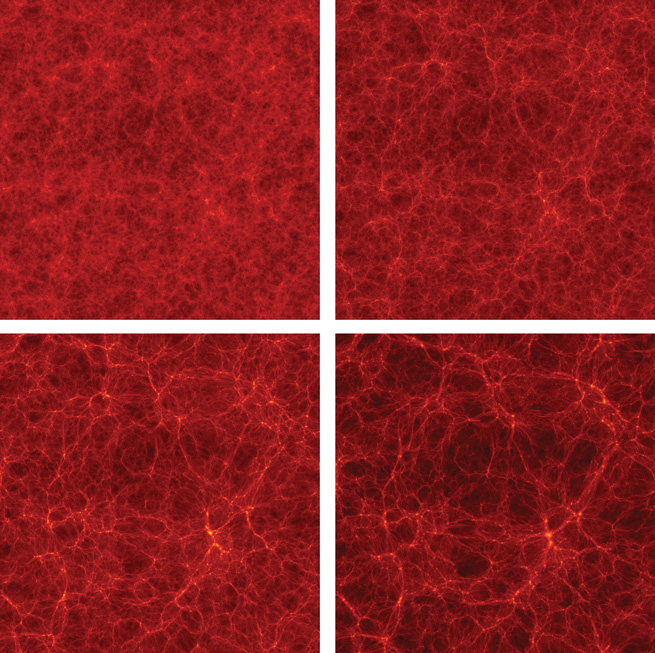
\includegraphics[width=0.85\textwidth]
	{./figures/3_nbody_simulations/Bolshoi_Evolution.png}

	\caption{\small{Evolución de la simulación Bolshoi. Se ilustran el
	campo de densidad de una región rectangular de 16 Mpc$/h$ de grosor y 
	250 Mpc$/h$	de lado para diferentes estadios de evolución. $z=9.5$ 
	(superior izquierda), $z=3$ (superior derecha), $z=1$ (inferior 
	izquierda) y $z=0$ (inferior derecha). Tomado de 
	\url{http://spectrum.ieee.org/aerospace/astrophysics/the-cosmological-supercomputer} }}
	
	\label{fig:Bolshoi_Evolution}
\end{figure}
%.........................................................................


Debido a su mayor tamaño comóvil comparada con las simulaciones 
restringidas (un cubo de $250$ Mpc$/h$ de lado), esta es usada para 
obtener estadística más fina en los resultados del capítulo 
\ref{cha:Results}. El modelo cosmológico usado para esta simulación 
corresponde al WMAP7 (ver tabla \ref{tab:CosmologicalParameters}), el número 
de partículas es de $2048^3$, lo que implica una masa promedio por partícula 
de $1.35 \times 10^8 h^{-1}$ M$_{\odot}$. Una descripción técnica más 
detallada de la simulación puede ser consultada en \cite{klypin2011}.
\newpage

	%---------------------------------------------------------------------
	%Constrained simulations (CLUES)
	\subsection{Simulaciones Restringidas (CLUES)}
	\label{subsec:ConstrainedSimulations}
	%---------------------------------------------------------------------


Como fue mencionado en el capítulo \ref{cha:Theoretical Framework}, la forma
estándar de comparar el resultado de simulaciones cosmológicas con 
observaciones es a través de las propiedades estadísticas de las 
distribuciones, tales como funciones de correlación de dos puntos o 
espectros de potencia. A pesar de esto, algunos estudios requieren una 
descripción detalla del universo local en un contexto cosmológico. Debido 
a dificultades técnicas como la medida directa de la distribución de materia
oscura o la falta de datos en altos corrimientos al rojo, es necesario 
recurrir a simulaciones cosmológicas que reproduzcan el universo local.
Uno de los primeros trabajos dirigidos a la reproducción específica del
entorno local se debe a \cite{Klypin2003}. En este se intenta reproducir las 
principales estructuras observadas en el universo local, como el grupo local,
el Supercúmulo Local y el cúmulo de Virgo.


%.........................................................................
%Constrained Simulation
\begin{figure}[htbp]
	\centering
	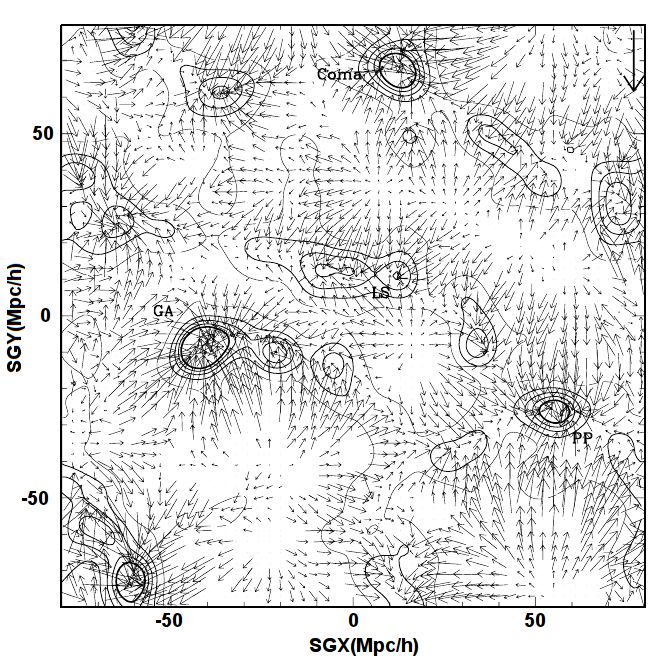
\includegraphics[width=0.60\textwidth]
	{./figures/3_nbody_simulations/Constrained_Construction.png}

	\caption{\small{Campo de densidad y campo de velocidad peculiar inicial
	construidos a partir de restricciones para la reproducción del entorno
	local en una escala de $160\ h^{-1}$Mpc. Algunas estructuras 
	identificadas son: \textit{Coma}, cúmulo de coma, \textit{PP}, supercúmulo 
	de Perseus-Pisces, \textit{LS}, supercúmulo local, \textit{GA}, gran 
	atractor. La flecha superior derecha indica la escala del campo de 
	velocidad peculiar en $1000$ km/s. Tomado de \cite{Klypin2003}.}}
	
	\label{fig:Constrained_Construction}
\end{figure}
%.........................................................................


El método propuesto en \cite{Klypin2003} y \cite{Hoffman1991} consiste en 
la construcción el campo de densidad y de velocidad peculiar inicial a 
partir de surveys de velocidades radiales y de corri\-mientos al rojo (ver 
sección \ref{sec:CosmologicalObservations}). Para el tratamiento y 
reducción del ruido y errores de medida en los datos, se usa un método 
bayesiano de filtros de Wiener (para más detalles técnicos ver 
\cite{Zaroubi1999}). A pequeñas escalas este método es limitado debido a 
que los filtros aplicados suprimen algunos modos en el espectro de potencia 
inicial y por tanto deben ser generados de forma aleatoria acorde con la 
distribución Gaussiana \ref{eq:GaussianDistribution} para garantizar 
consistencia con el modelo cosmológico estándar. En la figura 
\ref{fig:Constrained_Construction} se ilustran las condiciones iniciales 
obtenidas con este método para el universo local en una escala de 
$160\ h^{-1}$Mpc.


%.........................................................................
%CLUES Right Simulation
\begin{figure}[htbp]
	\centering
	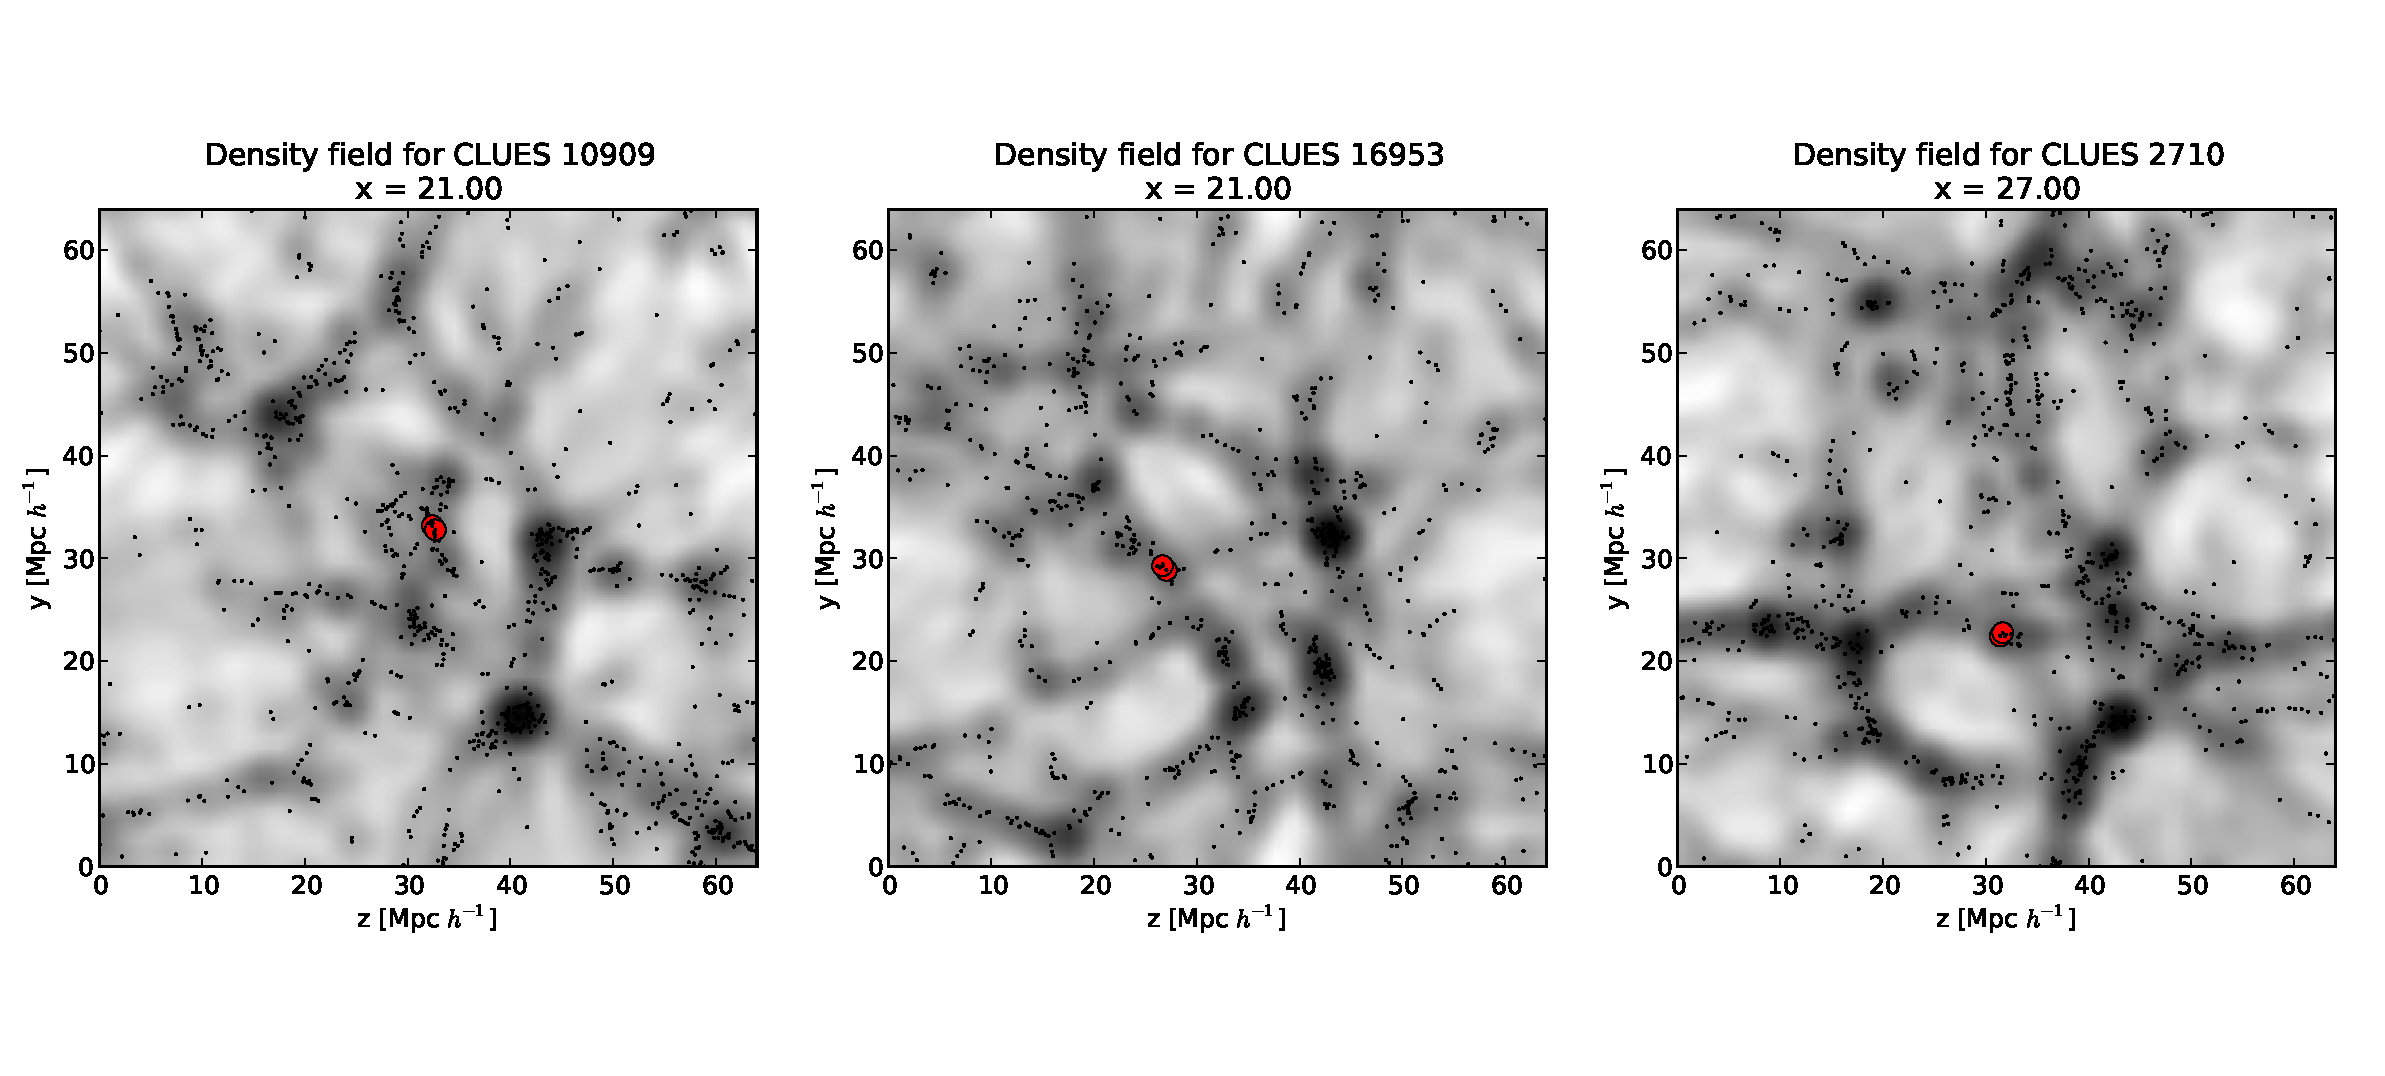
\includegraphics[width=1.0\textwidth]
	{./figures/3_nbody_simulations/CLUES_Simulations.pdf}

	\caption{\small{Tres simulaciones restringidas del proyecto CLUES 
	en las se identifican sistemas tipo grupo local. Se ilustra el campo 
	de densidad de cada simulación junto con los halos de materia oscura
	(puntos negros), y los grupos locales encontrados (puntos rojos).}}
	
	\label{fig:CLUES_Right}
\end{figure}
%.........................................................................


\textbf{CLUES} (Constrained Local UniversE Simulations) es un proyecto 
orientado a la reproducción del universo local con la mejor resolución 
en la actualidad. La página oficial es \url{http://www.clues-project.org}. 
En estas simulaciones las condiciones iniciales son construidas con el 
algoritmo Hoffman-Ribak \cite{Hoffman1991} para la reproducción de un 
volumen comóvil de $(64\ h^{-1}$Mpc$)^{3}$. Debido a la no restricción en
escalas pequeñas ($\sim 5\ h^{-1}$Mpc) es necesario realizar $200$ 
diferentes simulaciones de las cuales $3$ resultan satisfactorias 
respecto a las restricciones observacionales (ver figura 
\ref{fig:CLUES_Right}). Para la evolución se usa el paquete 
\texttt{GADGET2}\footnote{\texttt{GADGET2} es un popular código para la 
simulación de N-cuerpos en cosmología y formación de galaxias. Está 
disponible de forma gratuita en la página oficial del proyecto 
\url{http://www.mpa-garching.mpg.de/gadget/}} con $1024^3$ partículas de
materia oscura y una cosmología consistente con el WMAP7 (ver tabla 
\ref{tab:CosmologicalParameters}). Más detalles técnicos del proyecto
pueden ser consultados en \cite{Gottloeber2010}.


%.........................................................................
%CLUES Simulation Overview
\begin{figure}[htbp]
	\centering
	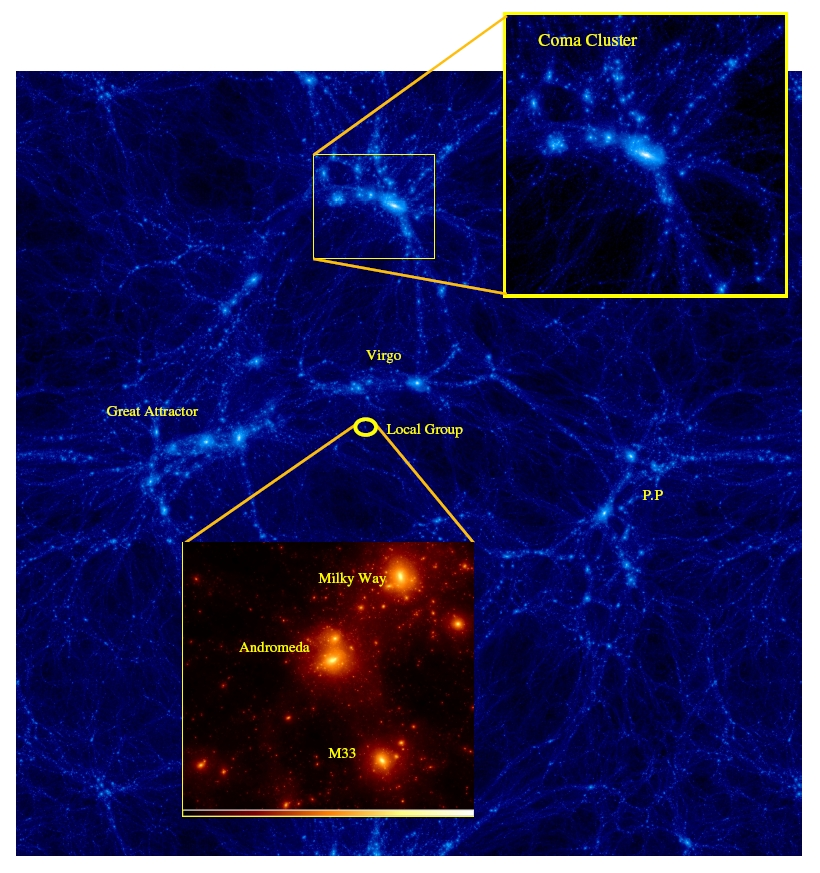
\includegraphics[width=0.90\textwidth]
	{./figures/3_nbody_simulations/CLUES_Overview.png}

	\caption{\small{Simulación obtenida en el proyecto CLUES. En esta se 
	muestran las estructuras a gran escala del universo local y se aprecian
	con claridad los miembros más significativos del grupo local. Tomado de 
	la 	página oficial del proyecto \url{http://www.clues-project.org}}}
	
	\label{fig:CLUES_Overview}
\end{figure}
%.........................................................................


%*************************************************************************



%*************************************************************************
%Environment Characterization
\section{Caracterización del Entorno}
\label{sec:EnvironmentCharacterization}


Una vez obtenidas las simulaciones numéricas de la evolución en régimen no 
lineal, uno de los principales objetivos es caracterizar las estructuras 
emergentes propias de este régimen. Entre estas destaca la gran estructura 
de red que se forma a partir de regiones de diferente dimensionalidad, 
donde grandes regiones vacías son limitadas por regiones planas, estas a 
su vez son recorridas por filamentos unidimensionales que se juntan en regiones 
puntuales altamente densas (red cósmica). 


A partir de observaciones cosmológicas se ha logrado establecer la 
relación entre las propiedades de halos de galaxias, tales como el parámetro 
de espín, la concentración, la forma, etc. Y el entorno donde están 
embebidas. Debido a esto es importante cuantificar la estructura de red 
cósmica en simulaciones cosmológicas. Uno de los primero trabajos en esta 
dirección consiste en la aproximación de Zeldovich mostrada en la subsección 
\ref{subsec:Zeldovich'sApproximation}), otros esquemas posteriores usan 
estratificaciones del campo de densidad para cuantificar el entorno y son 
denominados métodos geométricos, pero debido a su carácter local no 
pueden dar cuenta de propiedades más globales como canales de flujo de 
materia o influencia de grandes estructuras cercanas. En esta sección se 
muestran dos esquemas para la clasificación del entorno desarrollados 
recientemente.


	%---------------------------------------------------------------------
	%The T-web Method
	\subsection{Método T-web}
	\label{subsec:TheT-webMethod}
	%---------------------------------------------------------------------


El primero de los métodos fue propuesto por \cite{Hahn2007} y consiste el
uso de la teoría de sistemas dinámicos para el análisis de la estabilidad 
local de órbitas de prueba alrededor de halos de materia oscura y de esta 
forma cuantificar su entorno para un tiempo (corrimiento al rojo) fijo 
dado. Para esto se asume válida la aproximación Newtoniana (ver subsección 
\ref{subsec:Newtonian Approximation}) y la ecuación de movimiento de una 
partícula de prueba en el potencial peculiar de la distribución es


%.........................................................................
%Equation of Movement 
\eq{eq:Tweb_Movement}
{ \ddot{\bds r} = - \nabla \phi(\bds r) \ \ \ \ 
\mbox{con}\ \ \ \ \ \nabla^2 \phi = 4\pi G \bar \rho \delta}
%.........................................................................


Es razonable asumir que en el centro de masa $\bar{\bds r}_i$ de cada halo
existe un mínimo del potencial $\nabla \phi = 0$, formando así un pozo de 
potencial local. Esto permite linea\-lizar la ecuación de movimiento 
\ref{eq:Tweb_Movement} entorno a estos puntos, obteniendo


%.........................................................................
%Lineal Equation of Movement 
\eq{eq:Lineal_Tweb}
{ \ddot{r}_i = - T_{ij}(\bar{\bds r}_i)( r_j - \bar{ r}_{k,j})}
%.........................................................................
donde se define el tensor de marea como el Hessiano del potencial peculiar


%.........................................................................
%Tweb Tensor
\eq{eq:Tweb_Definition}
{ T_{ij} \equiv \frac{\partial^2 \phi}{\partial r_i \partial r_j}}
%.........................................................................


Acorde a la teoría de sistemas dinámicos, un autovalor negativo indica que
el punto es inestable en la dirección del respectivo autovector, implicando 
un flujo de materia hacia el exterior de la región. Para autovalores 
positivos se presenta una situación completamente análoga. Con base en la 
aproximación de Zeldovich (subsección \ref{subsec:Zeldovich'sApproximation})
se propone un esquema de clasificación del entorno cosmológico a partir de 
los autovalores del tensor de marea $T_{ij}$ 
(ver figura \ref{fig:ClassificationSchemeTweb}).


%.........................................................................
%Classification of Cosmological Environment
\begin{itemize}
\item \textbf{Vacío (Vacuum):} en este caso los tres autovalores son positivos, 
indicando una expansión en todas las direcciones.
\item \textbf{Hoja (Sheet):} para este caso $\lambda_1\geq\lambda_2>0$ y 
$\lambda_3<0$, indicando un colapso en una sola dirección, dando lugar a una 
zona con geometría local plana.
\item \textbf{Filamento (Filament):} para estas zonas solo el $\lambda_1$ es
positivo, indicando un colapso en dos direcciones y expansión e una, formando
así una región con geometría unidimensional.
\item \textbf{Nudo (Knot):} para este último tipo de región, los tres 
autovalores son negativos, indicando un colapso en todas las direcciones y 
dando lugar a una zona comprimida.
\end{itemize}
%.........................................................................


Lo más destacable de este método respecto a los métodos geométricos es su 
naturaleza dinámica, permitiendo diferenciar zonas con iguales valores 
densidad pero con propiedades de estabilidad diferentes. A pesar de lo 
anterior, la asunción de mínimo local solo es justificada en el centro de 
cada halo, careciendo así de significado y precisión generalizar este 
esquema en cualquier punto del espacio. Otro inconveniente es que bajo el 
esquema de clasificación original con los signos de cada autovalor no se 
reproduce la impresión visual que se obtiene en la distribución de materia
de las simulaciones (ver figura \ref{fig:TwebVwebComparison}).


%.........................................................................
%Classification Scheme
\begin{figure}[htbp]
	\centering
	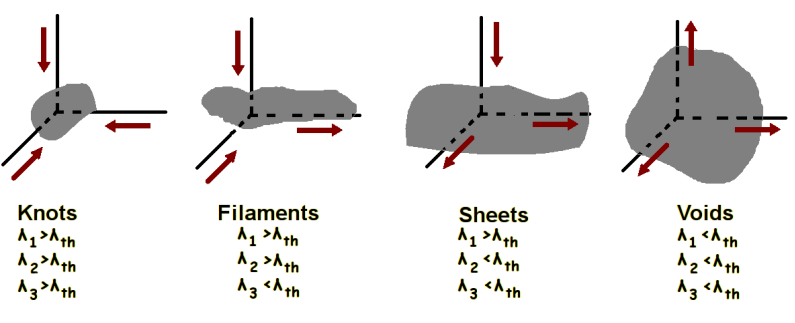
\includegraphics[width=0.9\textwidth]
	{./figures/2_theoretical_framework/EnvironmentClassification.png}

	\caption{\small{Esquema de clasificación del entorno cosmológico 
	para los esquemas T-web y V-web. El valor umbral $\lambda_{th}$ es 
	tomado como un parámetro libre.}}
	
	\label{fig:ClassificationSchemeTweb}
\end{figure}
%.........................................................................


Una significativa mejora de este método se logra generalizando el esquema 
de clasificación respecto a un cierto valor umbral $\lambda_{th}^T$, que 
es tomado como parámetro libre y se ajusta acorde a la impresión visual 
obtenida \cite{forero2008}, en especial el esquema original se recupera 
fijando $\lambda_{th}^T=0$.


	%---------------------------------------------------------------------
	%The V-web Method
	\subsection{Método V-web}
	\label{subsec:TheV-webMethod}
	%---------------------------------------------------------------------


El segundo método dinámico presentado para la clasificación de la red 
cósmica es presentado en \cite{hoffman2012} y está basado en el tensor de 
velocidad de peculiar (shear velocity tensor)


%.........................................................................
%Vweb Tensor
\eq{eq:Vweb_Definition}
{ \Sigma_{ij} = -\frac{1}{2 H_0}\pr{ \der{v_i}{r_j} + \der{v_j}{r_i} } }
%.........................................................................
de forma análoga al esquema T-web, en este esquema son calculados los 
auto\-valores del tensor $\Sigma_{ij}$ y se define el entorno acorde a un 
valor umbral $\lambda_{th}^V$ (ver figura \ref{fig:ClassificationSchemeTweb}).


Como es mostrado en \cite{hoffman2012}, en el régimen lineal los tensores
$T_{ij}$ y $\Sigma_{ij}$ son proporcionales, siendo ambos métodos 
completamente equivalentes en este régimen. Esto es parcialmente 
evidenciado en la impresión visual de ambos esquemas de clasificación que 
se obtiene a grandes escalas para la simulación Bolshoi (figura 
\ref{fig:TwebVwebComparison}), y se debe a la menor no linealidad de los 
modos a mayores escalas. 


%.........................................................................
%Tweb Vweb Comparison
\begin{figure}[htbp]
	\begin{center}
	\makebox[\textwidth]{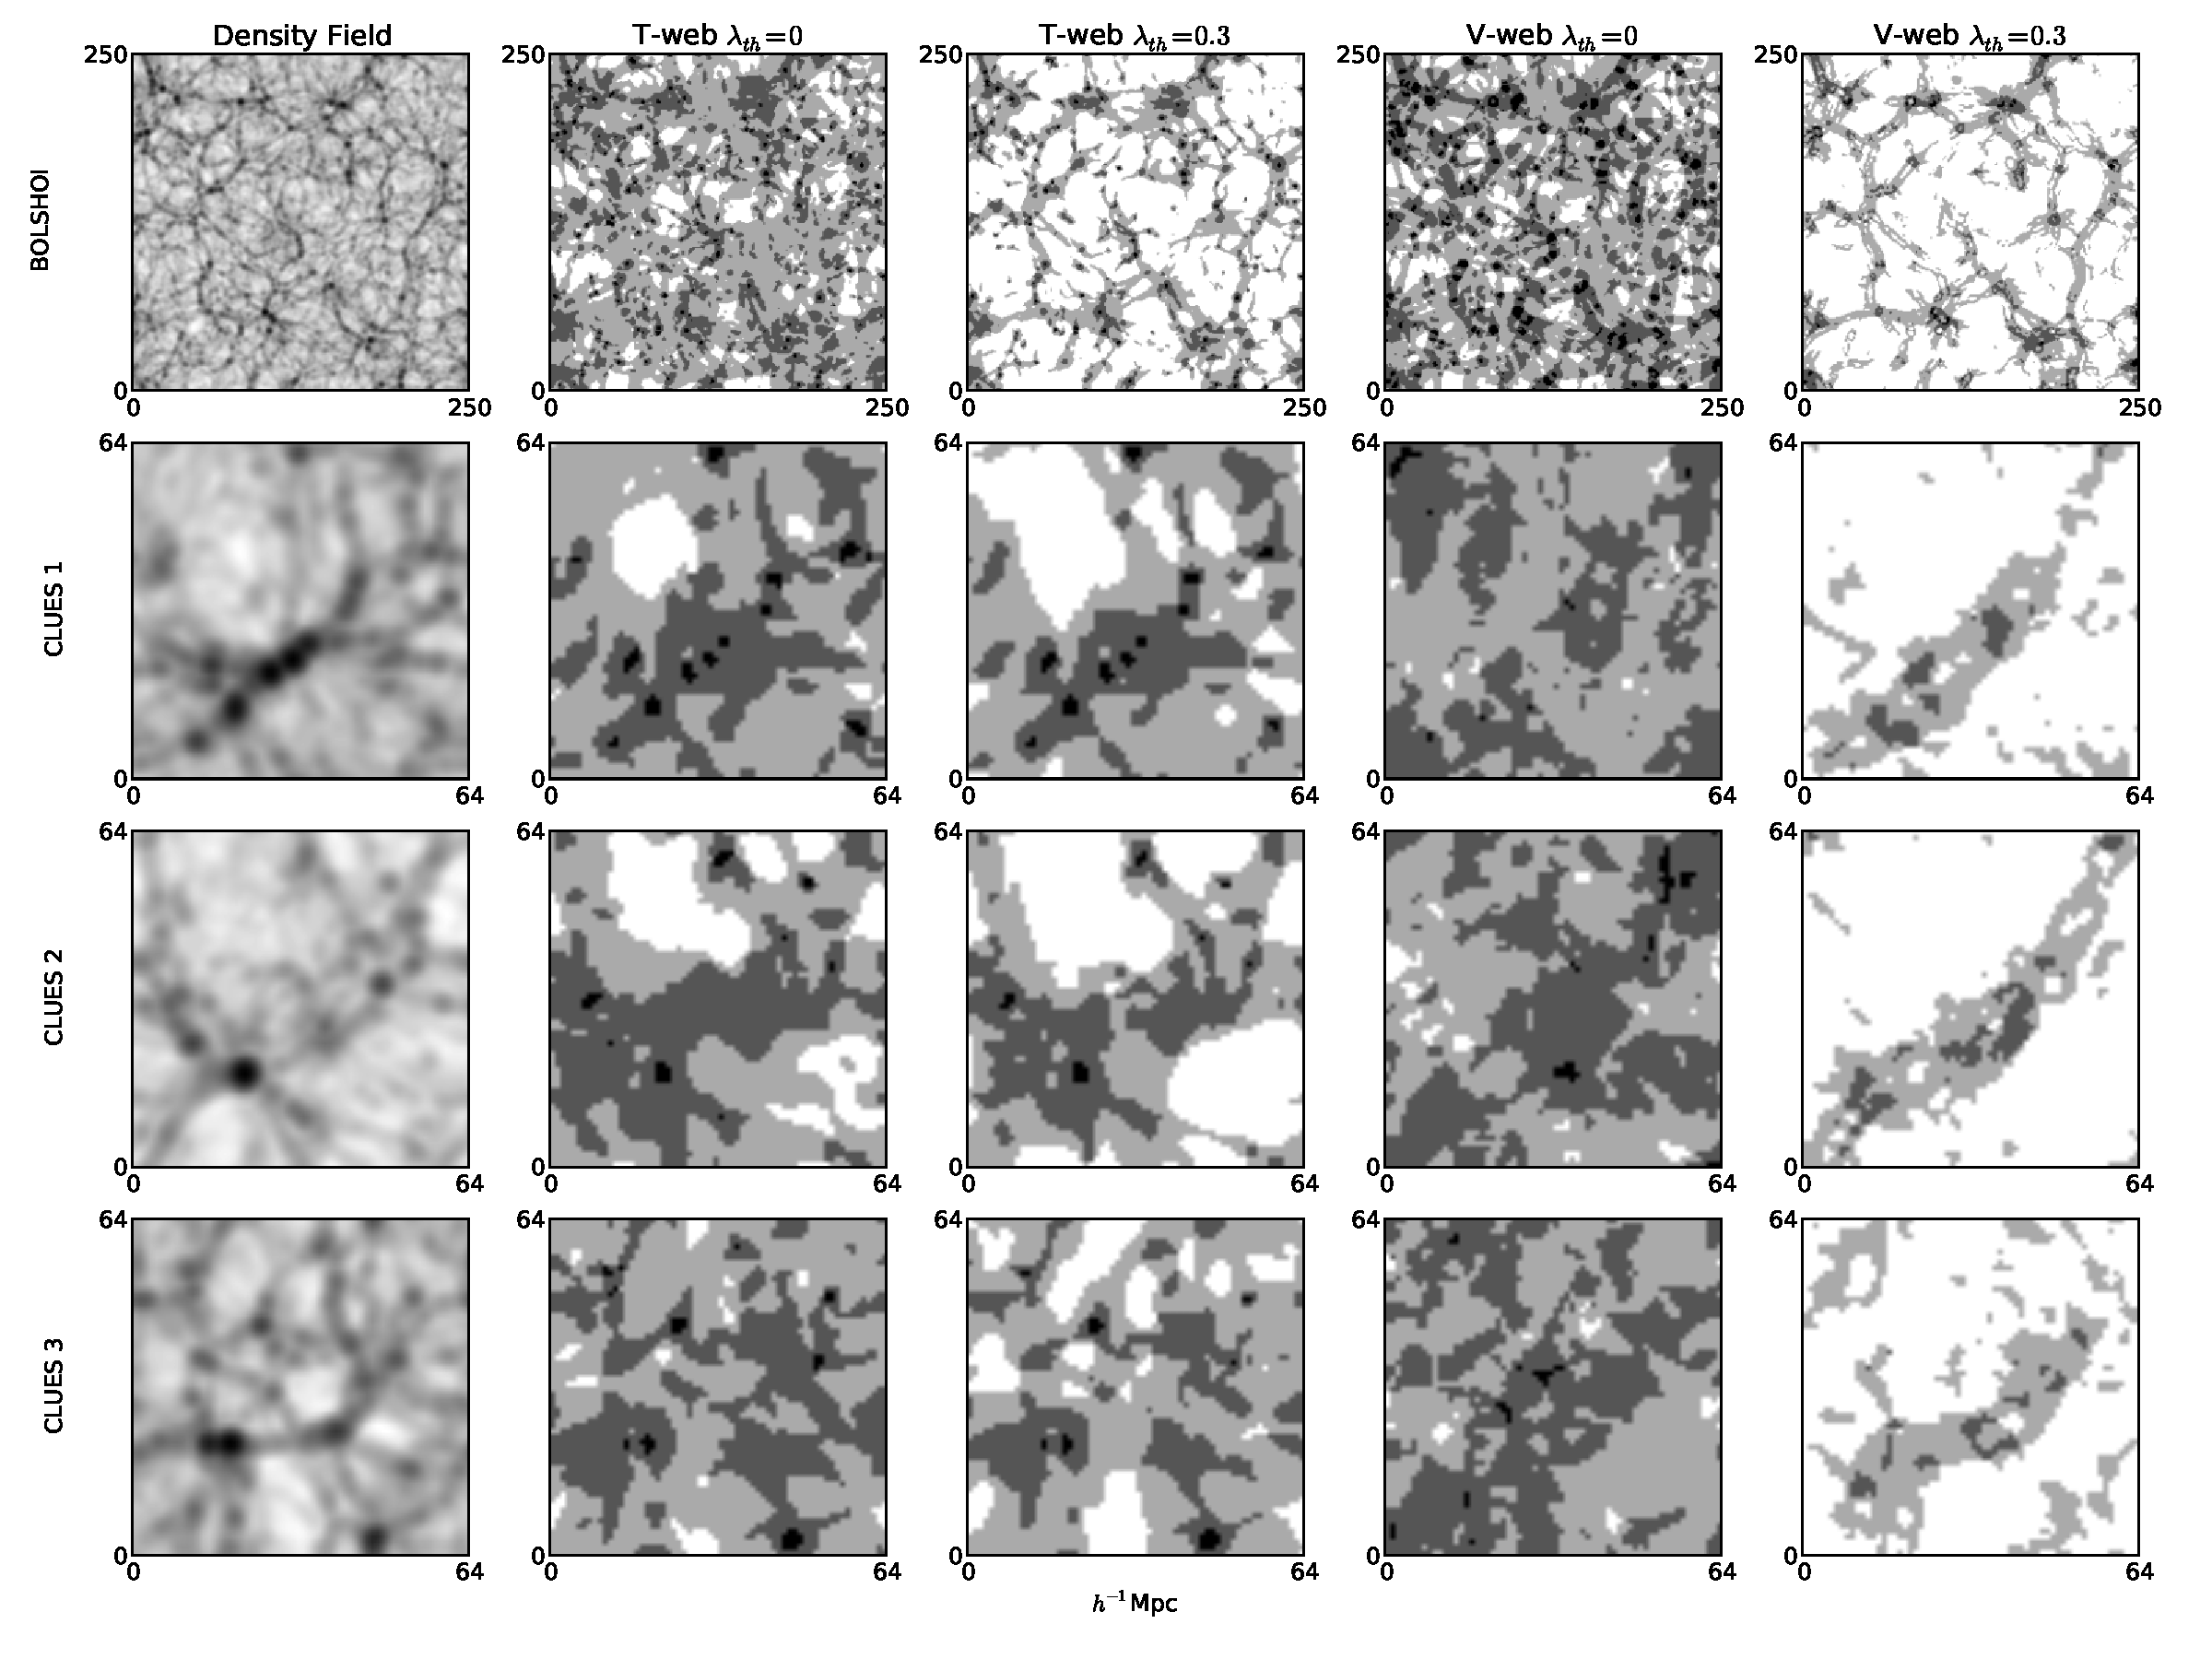
\includegraphics[trim = 5mm 8mm 10mm 5mm, clip, 
	width=0.80\paperwidth,angle=-90]
	{./figures/3_nbody_simulations/Vweb_Tweb.pdf}}
	\end{center}

	\caption{\small{Se ilustra para cada una las simulaciones
	(CLUES 1, CLUES 2, CLUES 3, Bolshoi) la diferencia entre los 
	esquemas de clasificación T-web y V-web para diferentes valores de 
	$\lambda_{th}$ (Negro - Nudo, Gris oscuro - Filamento, Gris - Hoja, 
	Blanco - Vacío). En las gráficas superiores se muestra la impresión 
	visual obtenida a partir de los respectivos campos de contraste de 
	densidad ($\log (\delta+1)$), usadas para la calibración de los valores 
	$\lambda_{th}$. La resolución para una de las mallas construidas es 
	aproximadamente $1.0 h^{-1}$ Mpc/celda y para todas se realiza un
	suavizado Gaussiano del tamaño de una celda, el grosor de cada slide
	es de una celda de la malla.}}
	
	\label{fig:TwebVwebComparison}
\end{figure}
%.........................................................................


En el caso de modos pequeños, donde los efectos no lineales son más 
do\-minantes, ambos esquemas difieren notablemente, tal como puede verse en 
la impresión visual de las simulaciones CLUES. Específicamente, el esquema 
V-web cuantifica de forma más precisa la estructura fina de la red 
cósmica a pequeñas escalas, permitiendo definir un entorno más apropiado 
para pequeñas estructuras a nivel cosmológico como halos de materia oscura 
o pequeños grupos de ellos.


Otra ventaja del esquema V-web respecto al T-web radica en que está basado 
en el campo de velocidades peculiares en vez del campo de densidad, aportando 
así más información dinámica del entorno y haciendo posible dar cuenta de una
forma más directa de efectos no locales, como flujos de materia o influencia 
de estructuras cercanas. Debido a esto, este esquema será adoptado como 
estándar para la cuantificación del entorno de halos y pares de halos 
(sistemas como el grupo local) y de las distribuciones de entorno 
cosmológico en el capítulo \ref{cha:Results}.


%*************************************************************************




%*************************************************************************
%Halos detection and sample definitions
\section{Detección de Halos y Definición de Muestras}
\label{sec:HalosDetectionAndSampleDefinitions}


Una vez caracterizado el entorno cosmológico, el siguiente paso es encontrar 
las estructuras que se forman en las simulaciones, específicamente halos de 
materia oscura. Debido a la naturaleza continua de la distribución de materia 
en el universo, es complicado y subjetivo definir estructuras discretas y 
limitadas espacialmente, como los halos de materia oscura o las galaxias en 
ellos. A pesar de esto, el carácter aproximado de las soluciones numéricas 
exige a priori uan construcción discreta del campo de densidad a partir de 
partículas puntuales con una cierta masa representativa (generalmente del 
orden de $10^7 \sim 10^9 h^{-1}$ M$_{\odot}$, aunque depende específicamente 
de la resolución de la simulación), esto implica que la detección de 
estructuras físicas discretas\footnote{A pesar de que las partículas que 
mapean la distribución de densidad también tienen un carácter discreto, su 
individualidad carece de sentido físico y solo es consecuencia de los 
métodos numéricos implementados.} se reduce a encontrar agrupaciones de 
partículas que representen estos sistemas.


	%---------------------------------------------------------------------
	%FOF method
	\subsection{Método FOF}
	\label{subsec:FOFMethod}
	%---------------------------------------------------------------------
	

Uno de los métodos más utilizados para la detección de estructuras en 
simulaciones de N-cuerpos se denomina FOF (por sus siglas en inglés
\textit{Friend of Friend}).

\
%.........................................................................
%FOF Method
\begin{figure}[htbp]
	\centering
	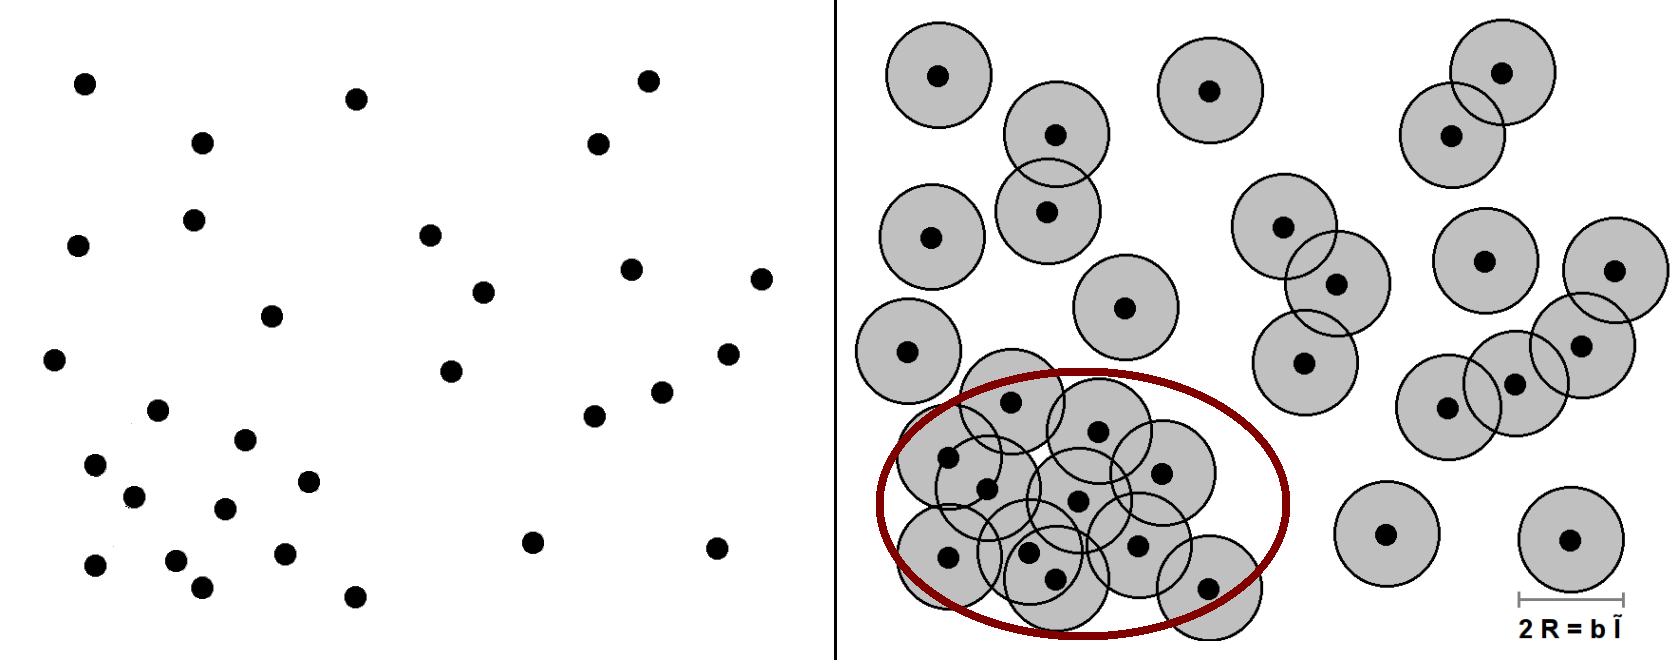
\includegraphics[width=0.9\textwidth]
	{./figures/3_nbody_simulations/FOF_Method.png}

	\caption{\small{Diagrama ilustrativo del método FOF. Los círculos grises
	entorno a cada partícula representa la zona de vinculación y la curva 
	roja representa una de las estructuras encontradas.}}
	
	\label{fig:FOF_Method}
\end{figure}
%.........................................................................


En este método se asocia un volumen finito a cada partícula, denominada 
región de vinculación, luego las estructuras son halladas a partir de 
intersecciones contiguas de estas regiones. Un ejemplo ilustrativo es 
presentado en la figura \ref{fig:FOF_Method}, donde la estructura de la curva
roja, correspondiente a un halo de materia oscura, es construida a partir
de 11 regiones de vinculación adyacentes que se intersectan mutuamente.
La geometría de las regiones de vinculación son generalmente esféricas, con
un radio $R_i$ dado por la siguiente expresión


%.........................................................................
%FOF Diameter
\eq{eq:FOF_Diameter}
{ R_i = \frac{1}{2}b\ \bar l }
%.........................................................................
donde $b$ es el parámetro de vinculación y $\bar l$ el camino libre medio 
de las partículas en la simulación. El parámetro de vinculación $b$ es libre 
y depende de cada simulación, siendo especificado a priori en la construcción 
de catálogos de halos.


En la figura \ref{fig:CLUES_FOF} se muestra el resultado del método FOF en
la construcción de un catálogo de halos de materia oscura para la simulación
CLUES 3. La distribución de los halos está acorde con la distribución de 
densidad (ver figura \ref{fig:TwebVwebComparison}), siguiendo el mismo patrón
de filamentos y nodos de la red cósmica. En el subsección 
\ref{subsec:SampleOfPairsToUse}, las muestras de halos definidas en cada 
simulación se hallan a partir de este esquema, con un parámetro de 
vinculación $b = 0.17$.


%.........................................................................
%FOF method in CLUES simulation
\begin{figure}[htbp]
	\centering
	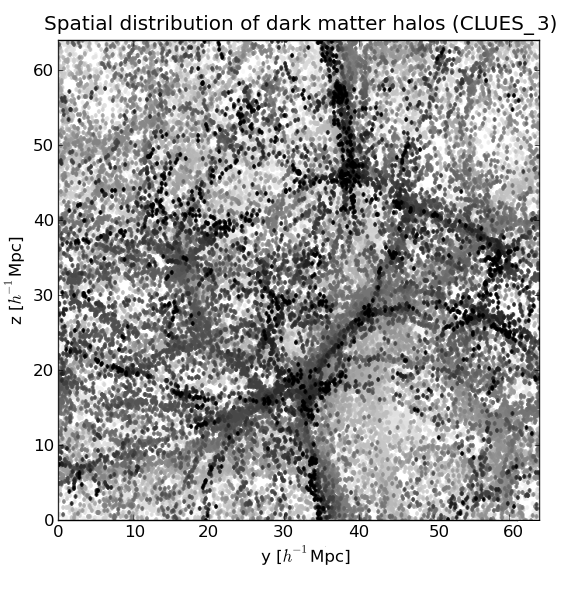
\includegraphics[width=0.5\textwidth]
	{./figures/3_nbody_simulations/Halos_Spatial_Distribution(CLUES_16953).png}

	\caption{\small{Halos encontrados a partir del esquema FOF en una de 
	las	simulaciones CLUES. El gradiente de color indica la profundidad 
	respecto al eje $x$, donde los halos negros son los más cercanos.}}
	
	\label{fig:CLUES_FOF}
\end{figure}
%.........................................................................


	%---------------------------------------------------------------------
	%Sample of pairs to use
	\subsection{Definición de Muestras}
	\label{subsec:SampleOfPairsToUse}
	%---------------------------------------------------------------------
	

En esta subsección se presentan las diferentes muestras definidas que serán 
usadas en el capítulo \ref{cha:Results} para la determinación de los efectos 
del entorno en los sistemas de grupos locales y la caracterización de cada 
simulación. Estas corresponde a una versión ampliada de las muestras 
definidas en \cite{forero2011}.


%.........................................................................
%Samples in All Simulations
\begin{itemize}
\item \textbf{Halos Generales} \textit{(GH)}\textbf{:} estos corresponden a
todos los halos hallados en las simulaciones a partir del esquema FOF, 
independiente de su rango de masa.

\item \textbf{Halos Individuales} \textit{(IH)}\textbf{:} son un subconjunto 
de la anterior muestra, y representan todos los halos de materia oscura que 
están en el rango de masas $5.0 \times 10^{11}\Msun - 5.0\times 10 ^{12}\Msun$. 
Este rango de masa es escogido debido a que corresponde al rango en el cual 
se forman galaxias de disco, tal como los principales miembros del grupo local,
Andrómeda y la Vía Láctea.

\item \textbf{Pares} \textit{(P)}\textbf{:} esta es construida a partir de 
la muestra \textit{IH} y está compuesta por pares de halos que satisfacen el 
criterio de ser mutuamente el halo más cercano al otro. Se construye como una 
muestra primigenia para encontrar sistemas de pares aislados y similares al 
grupo local.

\item \textbf{Pares Aislados} \textit{(IP)}\textbf{:} esta muestra se construye
a partir de los sistemas en la muestra de pares que además satisfacen las 
siguientes condiciones \cite{forero2011} \cite{forero2013}.


%.........................................................................
%CLG conditions
	\begin{itemize}
	\item La distancia entre el centro de los halos debe ser menor a 
	$0.7 h^{-1}$ Mpc, consistente con la distancia entre la Vía Láctea
	y Andrómeda.
	\item La velocidad radial relativa entre ambos halos debe ser negativa.
	\item No debe haber ningún objeto más masivo que alguno de los dos halos
	a una distancia menor que $2.0 h^{-1}$ Mpc de ambos.
	\item No debe existir ningún objeto más masivo que $5.0 \times 10^{13}\Msun$
	a una distancia menor que $5h^{-1}$ Mpc respecto a ambos halos.
	\end{itemize}
%.........................................................................	
	

Estas condiciones garantizan el aislamiento de los pares respecto a la 
influencia gravitacional de estructuras mayores y otros halos 

\item \textbf{Grupos Locales} \textit{(LG)}\textbf{:} esta muestra es 
definida en la simulaciones CLUES y corresponde a los pares de halos 
construidos a priori para la reproducción del grupo local. Por definición, 
solo existe un sistema \textit{LG} por cada una de las tres simulaciones 
CLUES.

\item \textbf{Grupos Locales Construidos} \textit{(CLG)}\textbf{:} con el
objetivo de obtener una muestra de sistemas tipo \textit{LG} en 
simulaciones no restringidas, se propone un método de construcción basado
en el entorno cosmológico de la muestra \textit{LG} en las simulaciones 
CLUES (ver figura \ref{fig:LG_Sample_Environment}). Para esto se calculan
los 3 campos de autovalores del \textit{shear velocity tensor} en una malla
con resolución de $1.0 h^{-1}$ Mpc/celda y un suavizado Gaussiano de una 
celda. En la siguiente tabla se tabulan los valores obtenidos para los 
autovalores del entorno de los sistemas \textit{LG}.


%.........................................................................
%Table of extreme values of LG environment
\begin{table}[htbp]
\begin{flushright}
\begin{minipage}[r]{0.9\textwidth}
\begin{small}
  \centering
  \begin{tabular}{| c | c | c | c |} \hline
	\cellc{\textbf{Descripción} } 				 				       & 
	\cellc{$\bds{\lambda_{1}}$ \footnotesize{$[10^{-1}]$}}   & 
	\cellc{$\bds{\lambda_{2}}$ \footnotesize{$[10^{-1}]$}}   & 
	\cellc{$\bds{\lambda_{3}}$ \footnotesize{$[10^{-1}]$}}   \\ \hline
	
	{CLUES 1\ H1} & 1.82 		& 1.20 				 	 & -1.59 \\
	{CLUES 1\ H2} & 1.82 		& 1.20 					 & -1.59 \\ \hline
	{CLUES 2 H1} & 1.78 		& 9.54$\times 10^{-1}$   & -8.85$\times 10^{-1}$ \\
	{CLUES 2 H2} & 2.19		& 4.45$\times 10^{-2}$   & -1.29 \\ \hline
	{CLUES 3 H1} & 3.23 		& -6.29$\times 10^{-2}$  & -1.98 \\
	{CLUES 3 H2} & 3.49 		& 1.21 					 & -1.29 \\ \hline
	{Valor mínimo} & 1.78 	& -6.29$\times 10^{-2}$  & -1.98 \\
	{Valor máximo} & 3.49 	& 1.21					 & -8.85$\times 10^{-1}$ \\ \hline
  \end{tabular}
  
  \caption{Autovalores asociados al entorno de cada grupo local en las simulaciones CLUES.}  
  \label{tab:Lambdas_LG}
\end{small}
\end{minipage}
\end{flushright}
\end{table}
%.........................................................................


%.........................................................................
%LG Environment in CLUES simulation
\begin{figure}[htbp]
\begin{flushright}
\begin{minipage}[r]{0.9\textwidth}
	\centering
	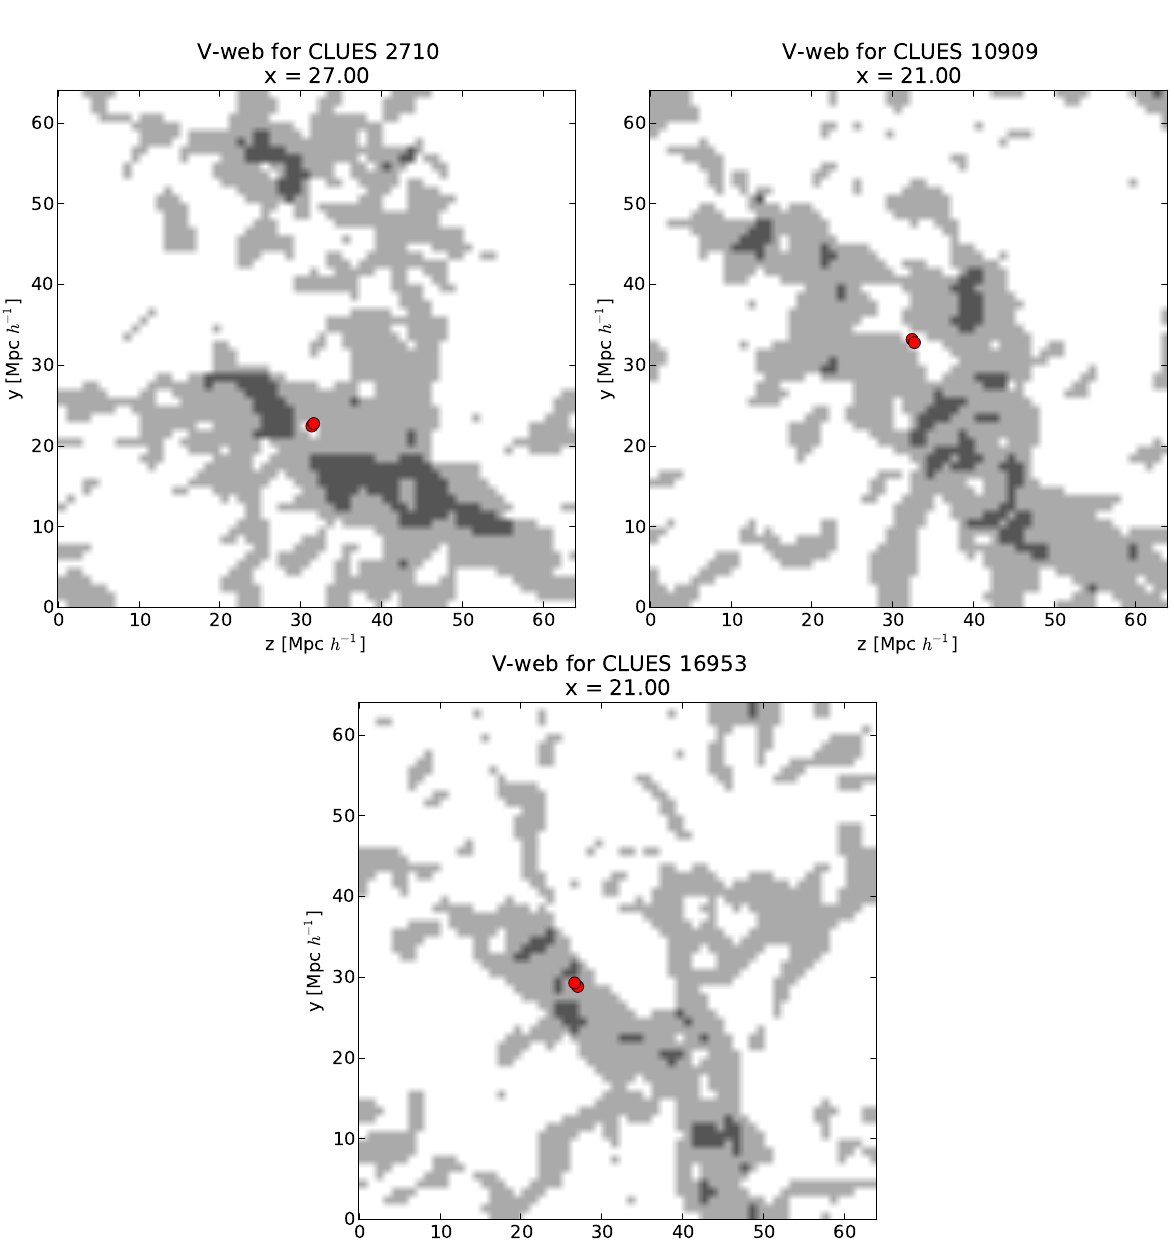
\includegraphics[width=0.75\textwidth]
	{./figures/3_nbody_simulations/LG_Environment.png}

	\caption{\small{Entorno cosmológico a partir del esquema V-web (con 
	$\lambda_{th} = 0.3$) para 	cada uno de los LG de las simulaciones 
	CLUES, indicados por los puntos	rojos.}}
	\label{fig:LG_Sample_Environment}
\end{minipage}
\end{flushright}
\end{figure}
%.........................................................................


Finalmente, a partir de los autovalores extremos hallados se define la 
muestra \textit{CLG} como aquellos pares \textit{IP} cuyos autovalores 
de entorno asociados se encuentran en el intervalo fijado. Para garantizar
autoconsistencia, esta muestra también es definida en las simulaciones 
CLUES.

\end{itemize}
%.........................................................................


%.........................................................................
%Table of samples numbers
\begin{table}[htbp]
\begin{small}
  \centering
  \begin{tabular}{| c | c | c | c | c |} \hline
	\cellc{\textbf{Muestra}}		& 
	\cellc{\textbf{CLUES 1}}		& 
	\cellc{\textbf{CLUES 2}} 		& 
	\cellc{\textbf{CLUES 3}}		& 
	\cellc{\textbf{Bolshoi}}		 \\ \hline
	\textit{GH} 	& 56632 & 57707 & 56799  & 432000 	\\
	\textit{IH}		& 1493 	& 1490 	& 1493	 & 88068 	\\
	\textit{P}		& 386 	& 380 	& 387	 & 23037 	\\
	\textit{IP}		& 20 	& 12 	& 18 	 & 1256 	\\
	\textit{LG}		& 1 	& 1 	& 1 	 & --		\\
	\textit{CLG}	& 1 	& 2 	& 3 	 & 30		\\ \hline
  \end{tabular}
  
  \caption{Tamaños de las muestras definidas para cada una de las 
  simulaciones. }  
  \label{tab:Samples}
\end{small}
\end{table}
%.........................................................................


Para finalizar, en la tabla \ref{tab:Samples} se tabula el tamaño de cada 
una de las muestras definidas para cada simulación. Puede notarse que 
los tamaños escalan aproxi\-madamente en la misma proporción que el 
volumen entre las simulaciones ($1/60$ -- CLUES /Bolshoi). En especial 
la muestra \textit{CLG} para Bolshoi tiene un tamaño proporcional
a la muestra \textit{LG} de las CLUES, indicando que el esquema de 
construcción propuesto reproduce sistemas tipo LG en simulaciones no 
restringidas.


	%---------------------------------------------------------------------
	%Sample Detection Method
	\subsection{Método de Detección de Pares}
	\label{subsec:Pairs_Detection}
	%---------------------------------------------------------------------
	

A continuación se describe el algoritmo desarrollado para la detección de 
cada una de las muestras de pares en cada simulación (\texttt{Pair Finder})
\footnote{Una versión actualizada del código puede encontrarse en 
\url{https://github.com/sbustamante/Thesis/tree/master/codes/Halo_Finder}}.

%.........................................................................
%Algorithm of pair finder
\begin{itemize}
\item Se particiona el espacio de la simulación en $N\times N \times N$
celdas, luego para cada celda se realiza un indexado de los halos que están 
dentro de ella, almacenando los identificadores de cada uno de ellos.

\item Posteriormente, para cada una de las celdas se identifican los 
primeros vecinos, teniendo en cuenta condiciones de frontera periódicas,
tal como la celda $i$ en la figura \ref{fig:Pair_Finder}.

\item Para un halo de una celda dada se calcula la distancia a todos los
halos de la misma celda y de las celdas vecinas, luego se almacena la 
distancia al halo más cercano, la distancia al halo más cercano con una 
masa mayor y la distancia al halo más cercano con una masa mayor a 
$5.0 \times 10^{13}\Msun$.

\item Repitiendo el anterior paso para todos los halos, si dos halos son
mutuamente los dos más cercanos, estos se catalogan como un par, 
construyendo así la muestra \textit{P} definida en la subsección anterior 
\ref{subsec:SampleOfPairsToUse}.

\item Finalmente, para cada uno de los sistemas de pares se evalúan las 
condiciones definitorias de los \textit{IP}, determinando así esta 
muestra.
\end{itemize}
%.........................................................................


%.........................................................................
%Pair Finder Diagram
\begin{figure}[htbp]
	\centering
	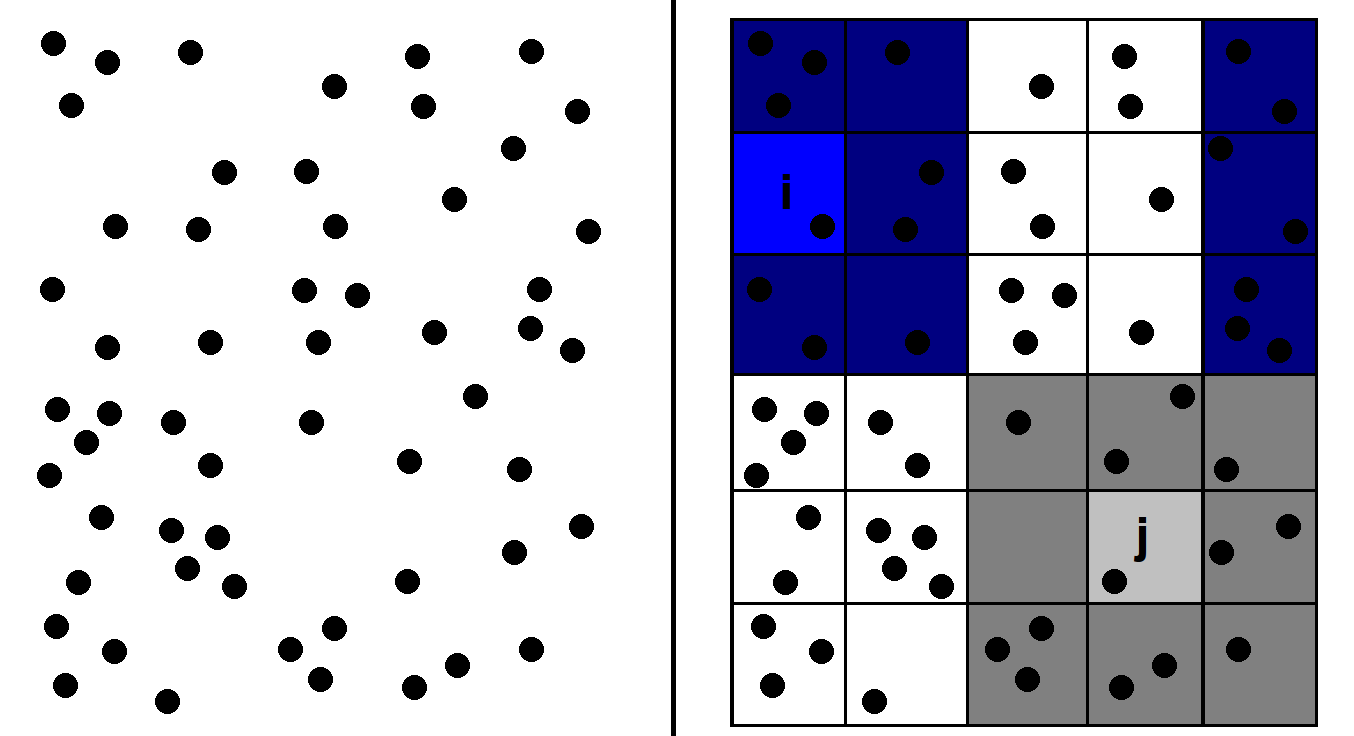
\includegraphics[width=0.6\textwidth]
	{./figures/3_nbody_simulations/PairFinder.png}

	\caption{\small{Ilustración 2D del método para la detección de las 
	muestras de pares. Distribución de halos de materia oscura (izquierda), 
	definición de zonas (derecha).}}
	\label{fig:Pair_Finder}
\end{figure}
%.........................................................................


La eficiencia de este método radica en que evita evaluar distancias entre 
todos los halos de la simulación, siendo necesario solo para los 
vecinos cercanos. La estructura de celdas lo hace similar a un 
código de árbol (ver subsección \ref{subsec:P3Method}), a excepción de la 
estructura jerárquica de este último. En principio, el código debe ser más
eficiente a medida que se aumenta la resolución $N$ de la malla, pero 
existen dos limitaciones que a esto. La primera tiene que ver con el 
número de halos por celda, este no puede ser demasiado grande, pero tampoco 
puede ser tal que solo hallan unos pocos halos por celda \footnote{Este
umbral no es bien definido y depende de cada simulación, por ejemplo para
las simulaciones usadas (Bolshoi y CLUES), un valor de $N=8$ es generalmente 
adecuado.}. La segunda limitación tiene que ver con las condiciones de 
distancia usadas en la definición de la muestra \textit{IP}, el tamaño 
físico de cada celda no puede ser menor a ninguna de estas distancias.


%*************************************************************************
			
%--------------------------- results ----------------------------
%qqqqqqqqqqqqqqqqqqqqqqqqqqqqqqqqqqqqqqqqqqqqqqqqqqqqqqqqqqqqqqqqqqqqqqqqq
%Quote
\begin{savequote}[50mm]
‘‘The most incomprehensible thing about the universe is comprehensible’’
\qauthor{Albert Einstein}
\end{savequote}
%qqqqqqqqqqqqqqqqqqqqqqqqqqqqqqqqqqqqqqqqqqqqqqqqqqqqqqqqqqqqqqqqqqqqqqqqq




%#########################################################################
\chapter{The Cosmological Environment and the Local Group}
\label{cha:Results}


%Reviewed
Next, it is presented the results obtained from the simulations described 
in the previous chapter \ref{cha:N-BodySimulations} for the dependence
of the properties of LG-like systems on the cosmological environment in 
which they are embedded. It is firstly characterized each one of the used
simulations (CLUES and Bolshoi) with the aim to guarantee consistency 
between the used cosmologies and between the distribution of the 
environmental properties (see section 
\ref{sec:StatisticalPropertiesOfAllSimulations}). After of this, in the 
section \ref{sec:PropertiesOfSamplePairs} it is determined the physical
and statistical properties of each one of the defined samples in
\ref{subsec:SampleOfPairsToUse} and it is analysed the correlations 
between the computed properties and the cosmological environment of each 
simulation.



%#########################################################################




%*************************************************************************
%Statistical properties of all simulations
\section{Propiedades de las Simulaciones}
\label{sec:StatisticalPropertiesOfAllSimulations}


Uno de los principales objetivos para determinar la influencia del entorno
sobre sistemas tipo grupo local es construir una muestra \textit{CLG} 
en simulaciones no res\-tringidas y así obtener estadística significativa. 
Para garantizar la consistencia de esta muestra es necesario
establecer la equivalencia entre las entre las distribuciones de halos 
oscuros y analizar las distribuciones de entorno cosmológico para cada 
simulación.


	%---------------------------------------------------------------------
	%Halos Properties
	\subsection{Función de Masa de los Halos}
	\label{subsec:Halos_Properties}
	%---------------------------------------------------------------------


La distribución espacial de los halos refleja la fina estructura de la red 
cósmica formada por la materia oscura, tanto en simulaciones (ver figura 
\ref{fig:Halos_Web}) como en observaciones cosmológicas (ver sección 
\ref{sec:CosmologicalObservations}). Esto sugiere posibles correlaciones 
entre las propiedades de los halos y el entorno en el cual están embebidos, 
tal como es mostrado para la forma de los halos, el parámetro de espín y 
alineación de subhalos en \cite{libeskind2013}, y para la masa de los halos 
\cite{lemson1999}. En especial el trabajo de \cite{libeskind2013} demuestra 
que el esquema de clasificación V-web es el más apropiado para estudios de 
correlaciones con propiedades direccionales, tal como el momento angular de 
los sistemas \textit{IP} o \textit{CLG} en la sección
\ref{sec:PropertiesOfSamplePairs}.

\
%.........................................................................
%FOF method in CLUES simulation
\begin{figure}[htbp]
	\centering
	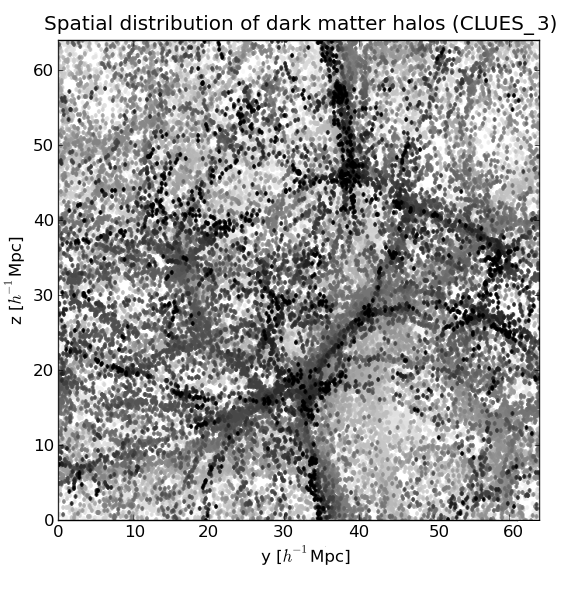
\includegraphics[width=0.55\textwidth]
	{./figures/3_nbody_simulations/Halos_Spatial_Distribution(CLUES_16953).png}

	\caption{\small{Distribución espacial de los halos de materia oscura, 
	reflejando la estructura de la red cósmica. El gradiente de color 
	indica la profundidad respecto al eje $x$, donde los halos negros son 
	los más cercanos.}}
	
	\label{fig:Halos_Web}
\end{figure}
%.........................................................................


Acorde a las condiciones definitorias de las muestras \textit{IP} y 
\textit{CLG} presentadas en la subsección \ref{subsec:SampleOfPairsToUse}, 
la principal propiedad de los halos necesaria para la construcción de estas 
muestras es la masa. Por esta razón es importante establecer la equivalencia 
entre las distribuciones de masa en cada simulación. En la siguiente figura 
\ref{fig:IMF} se calculan las funciones integradas de masa para la simulación 
Bolshoi y para las tres simulaciones CLUES.


%.........................................................................
%Integrated Mass Fraction
\begin{figure}[htbp]
	\centering
	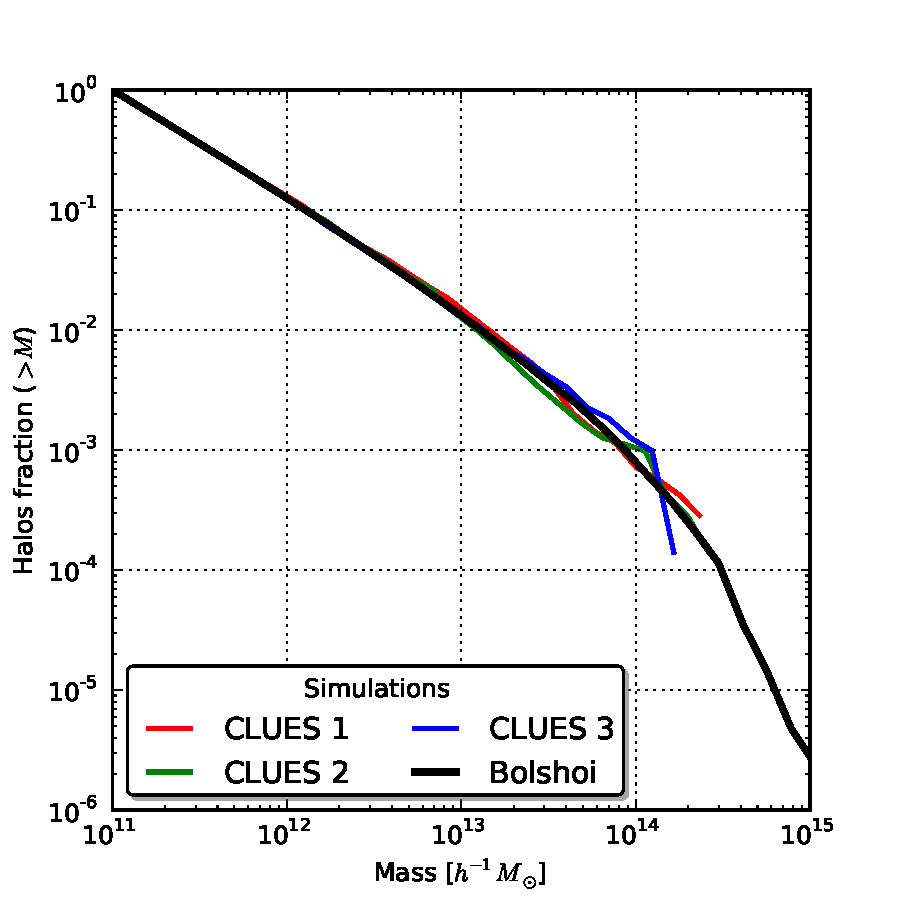
\includegraphics[width=0.70\textwidth]
	{./figures/4_results/Halos_IMF.pdf}
	
	\caption{\small{Funciones de masa integrada de halos de materia oscura 
	(muestra GH) para cada simulación.}}
	\label{fig:IMF}
\end{figure}
%.........................................................................


Para valores de masa altos las distribuciones son ligeramente diferentes 
debido a la menor cantidad de datos en las simulaciones CLUES, lo que hace
menos significativa la estadística en este caso. A pesar de esto, en el
rango masa donde son definidas las muestras \textit{IH} 
($5.0 \times 10^{11}\Msun - 5.0\times 10 ^{12}\Msun$) las distribuciones 
son consistentes con el formalismo Press-Schechter \cite{press1974} para 
los parámetros cosmológicos WMAP7, indicando así la equivalencia de las 
muestras definidas entre las simulaciones.


	%---------------------------------------------------------------------
	%Environment Properties
	\subsection{Distribución del Entorno Cosmológico}
	\label{subsec:Environment_Properties}
	%---------------------------------------------------------------------


Como fue mostrado en la sección \ref{sec:EnvironmentCharacterization}, 
la caracterización del entorno cosmológico se logra a partir de cantidades
físicas que indiquen el carácter geométrico o dinámico local de una región
de la distribución de materia. En especial el esquema V-web permite dar 
cuenta de la dinámica a pequeñas escalas de la estructura de la red cósmica,
permitiendo definir un entorno adecuado para los halos y otros sistemas.
En la siguiente figura son calculadas las distribuciones para cada uno de 
los autovalores de la V-web (distribuciones de entorno), tanto para las 
celdas de las simulaciones, como para los entornos de los halos de la 
muestra \textit{GH}.


%.........................................................................
%1D Distribution of Vweb eigenvalues in cells
\begin{figure}[htbp]
	\centering
	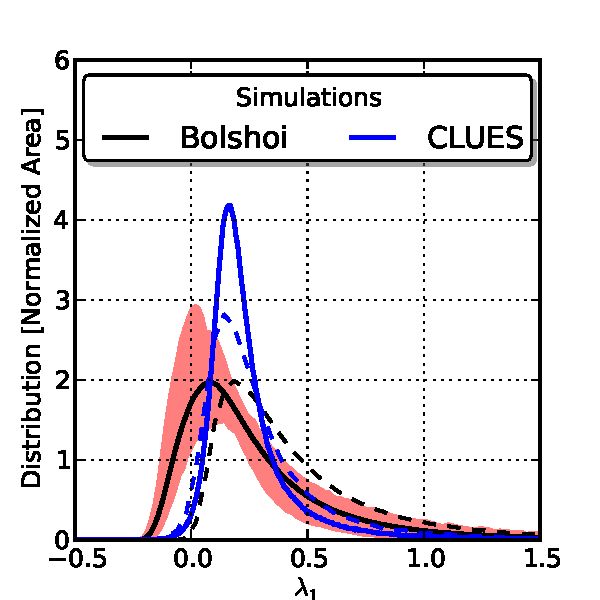
\includegraphics[width=0.4\textwidth]
	{./figures/4_results/Cells_Distro_L1.pdf}
	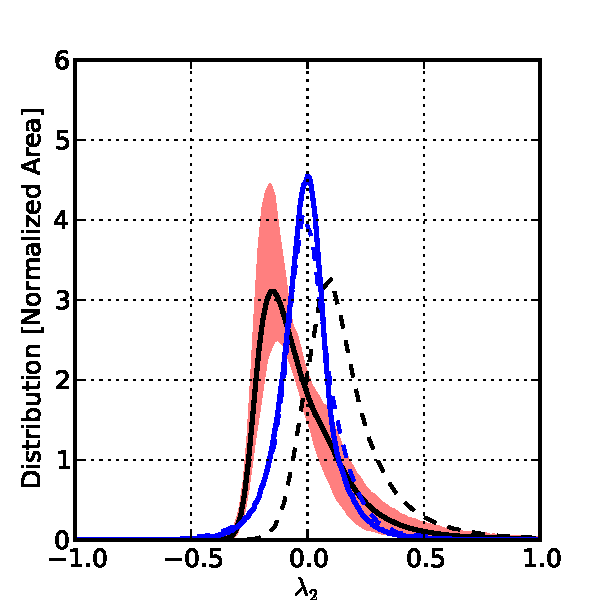
\includegraphics[width=0.4\textwidth]
	{./figures/4_results/Cells_Distro_L2.pdf}
	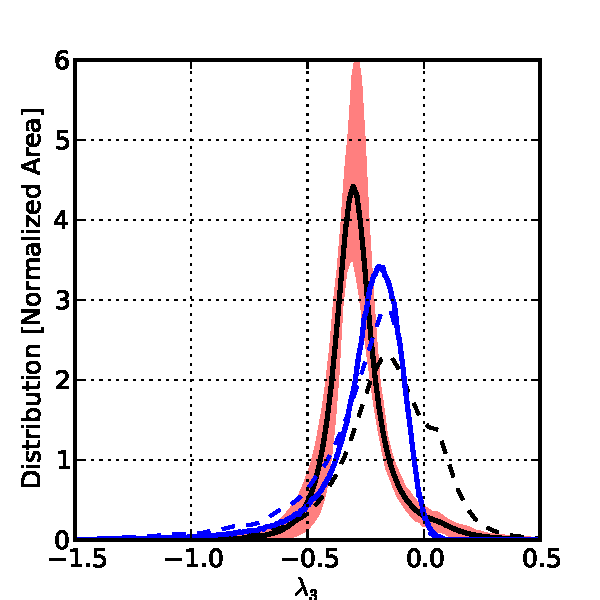
\includegraphics[width=0.4\textwidth]
	{./figures/4_results/Cells_Distro_L3.pdf}

	\caption{\small{ Distribución de los autovalores en el esquema V-web
	para cada una de las celdas de volumen (línea continua) y para los 
	entornos de los halos de materia oscura en los catálogos FOF (línea 
	discontinua). Las distribuciones están normalizadas tal que su área es
	la unidad. Resolución de $1.0 h^{-1}$ Mpc/celda y suavizado Gaussiano
	de una celda.}}
	\label{fig:1D_Cells_Eigenvalues}
\end{figure}
%.........................................................................


El principal resultado de la figura \ref{fig:1D_Cells_Eigenvalues} consiste 
en la diferencia de las distribuciones para las celdas de volumen (líneas 
continuas) entre la simulación Bolshoi y las simu\-laciones CLUES
\footnote{Debido a la alta semejanza entre las distribuciones de las tres
simulaciones CLUES, y con el fin de obtener estadística más significativa,
se han fusionado las distribuciones.}. El efecto de varianza cósmica 
(regiones rojas) es incluido a partir del cálculo de distribuciones de 
entorno en $64$ subvolúmenes de la simulación Bolshoi, con un tamaño similar 
a una simulación CLUES. A pesar de esto, las distribuciones de CLUES están 
por fuera de la región de varianza cósmica, indicando así una estructura 
cosmológica a gran escala que difiere entre ambas simulaciones.


Un segundo resultado importante de la figura \ref{fig:1D_Cells_Eigenvalues}
se obtiene a partir de las distribuciones de entorno para los halos 
(líneas discontinuas). En el caso de Bolshoi, se nota un importante
sesgo entre la distribución de entorno de las celdas y de los halos, 
indicando así que la distribución espacial de los halos no es un buen 
trazador de la estructura a gran escala del campo de densidad. Este 
resultado es consistente con el trabajo de \cite{libeskind2013}, donde 
hallan importantes sesgos en las distribuciones de entorno acorde a 
diferentes rangos de masa de los halos, también usando Bolshoi. En el 
caso de las simulaciones CLUES, las distribuciones de entorno de los 
halos son significativamente menos sesgadas respecto a las de celdas de 
volumen, indicando para este caso que los halos si se distribuyen 
espacialmente acorde al entorno cosmológico cuantificado por el esquema 
V-web.


Por último, en la figura \ref{fig:Vol_Fraction} son calculadas las 
densidades medias y las fracciones de volumen para cada uno de los tipos 
de regiones (ver sección \ref{sec:EnvironmentCharacterization}) acorde al 
valor umbral $\lambda_{th}$. Las funciones de fracción de volumen son 
diferentes entre las simulaciones CLUES y Bolshoi, en especial la región 
en torno a $\lambda_{th} = 0.1$ para las regiones tipo hoja (sheet). Esto se 
debe al desplazamiento relativo entre los picos de las distribuciones de 
entorno para cada simulación (ver figura \ref{fig:1D_Cells_Eigenvalues}), 
lo que implica un comportamiento diferente al criterio de selección de 
regiones a partir del valor $\lambda_{th}$. A pesar de esto, las fracciones 
de volumen se mantienen más o menos consistentes para ambas simulaciones 
en el rango  $0.2 \leq \lambda_{th} \leq 0.4$, que corresponde al rango 
donde mejor se reproduce visualmente la distribución global del campo de 
densidad.

\newpage
%.........................................................................
%Volume Fraction
\begin{figure}[htbp]
	\centering
	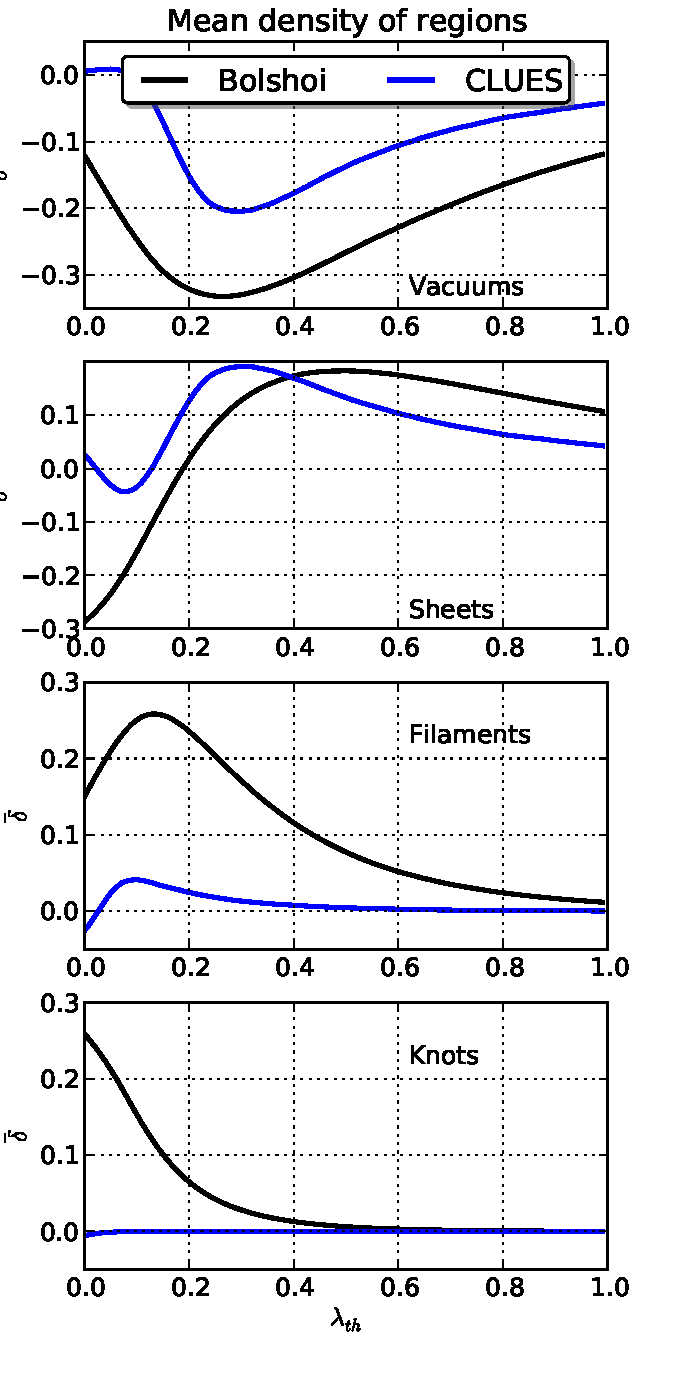
\includegraphics[width=0.43\textwidth]
	{./figures/4_results/Density_Regions.pdf}
	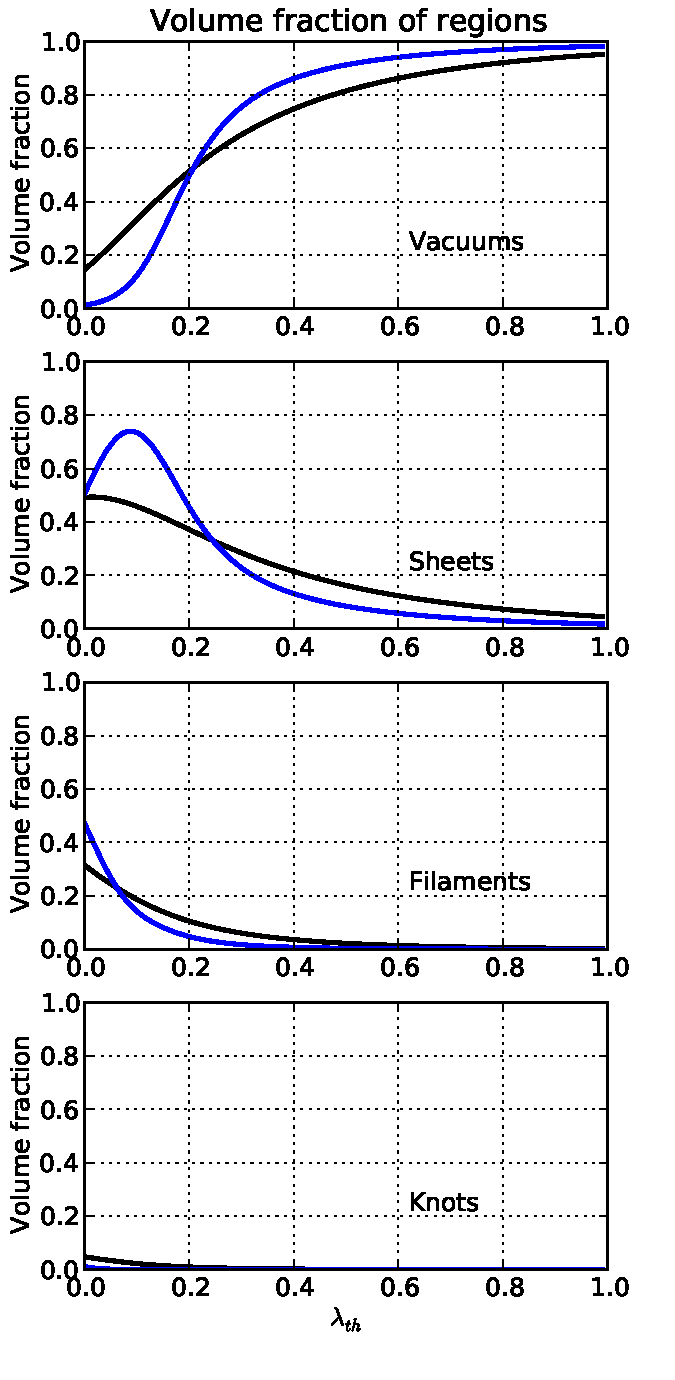
\includegraphics[width=0.43\textwidth]
	{./figures/4_results/Volume_Regions.pdf}
	
	\caption{\small{Parámetro de densidad medio para diferentes tipos
	de regiones en función del valor umbral $\lambda_{th}$ (paneles 
	izquierda). Fracciones de volumen normalizadas para diferentes tipos
	de regiones, también acorde al valor umbral $\lambda_{th}$.}}
	\label{fig:Vol_Fraction}
\end{figure}
%.........................................................................


Las gráficas de densidad media para cada tipo de región muestran 
importantes resultados respecto al entorno cosmológico. Lo primero que 
puede notarse es la diferencia entre las densidades medias de ambas 
simulaciones en cada una de las regiones. Por ejemplo para regiones de 
vacío, en Bolshoi estas corresponden a zonas con densidad promedio mucho 
menor a la densidad media de la simulación, mientras que para las CLUES 
estas zonas de subdensidad no son tan marcadas. Debido a la pequeña 
fracción de volumen de las regiones tipo nudo (knot) en ambas 
simu\-laciones, asociado a su dimensionalidad puntual, la estructura 
global del entorno puede entenderse bien solo en términos de la 
distribución espacial de vacíos, hojas y filamentos, siendo los 
filamentos la contraparte de los vacíos respecto al parámetro de densidad. 
De esto se espera que la diferencia en la subdensidad de los vacíos entre
cada simulación se extienda a una marcada diferencia entre las 
sobredensidades de los filamentos en cada simulación. Esto último es 
obtenido en la misma figura, donde puede verse que los filamentos de 
Bolshoi son notablemente más densos que aquellos de las CLUES. En el caso
de las hojas, estas corresponden a regiones de densidad intermedias entre
los filamentos y los vacíos, por tanto se espera que la diferencia de
la densidad media de estas regiones no sea tan marcada entre ambas 
simulaciones, tal como se nota en la misma figura.


%.........................................................................
%Vweb Comparison
\begin{figure}[htbp]
	\begin{center}
	\makebox[\textwidth]{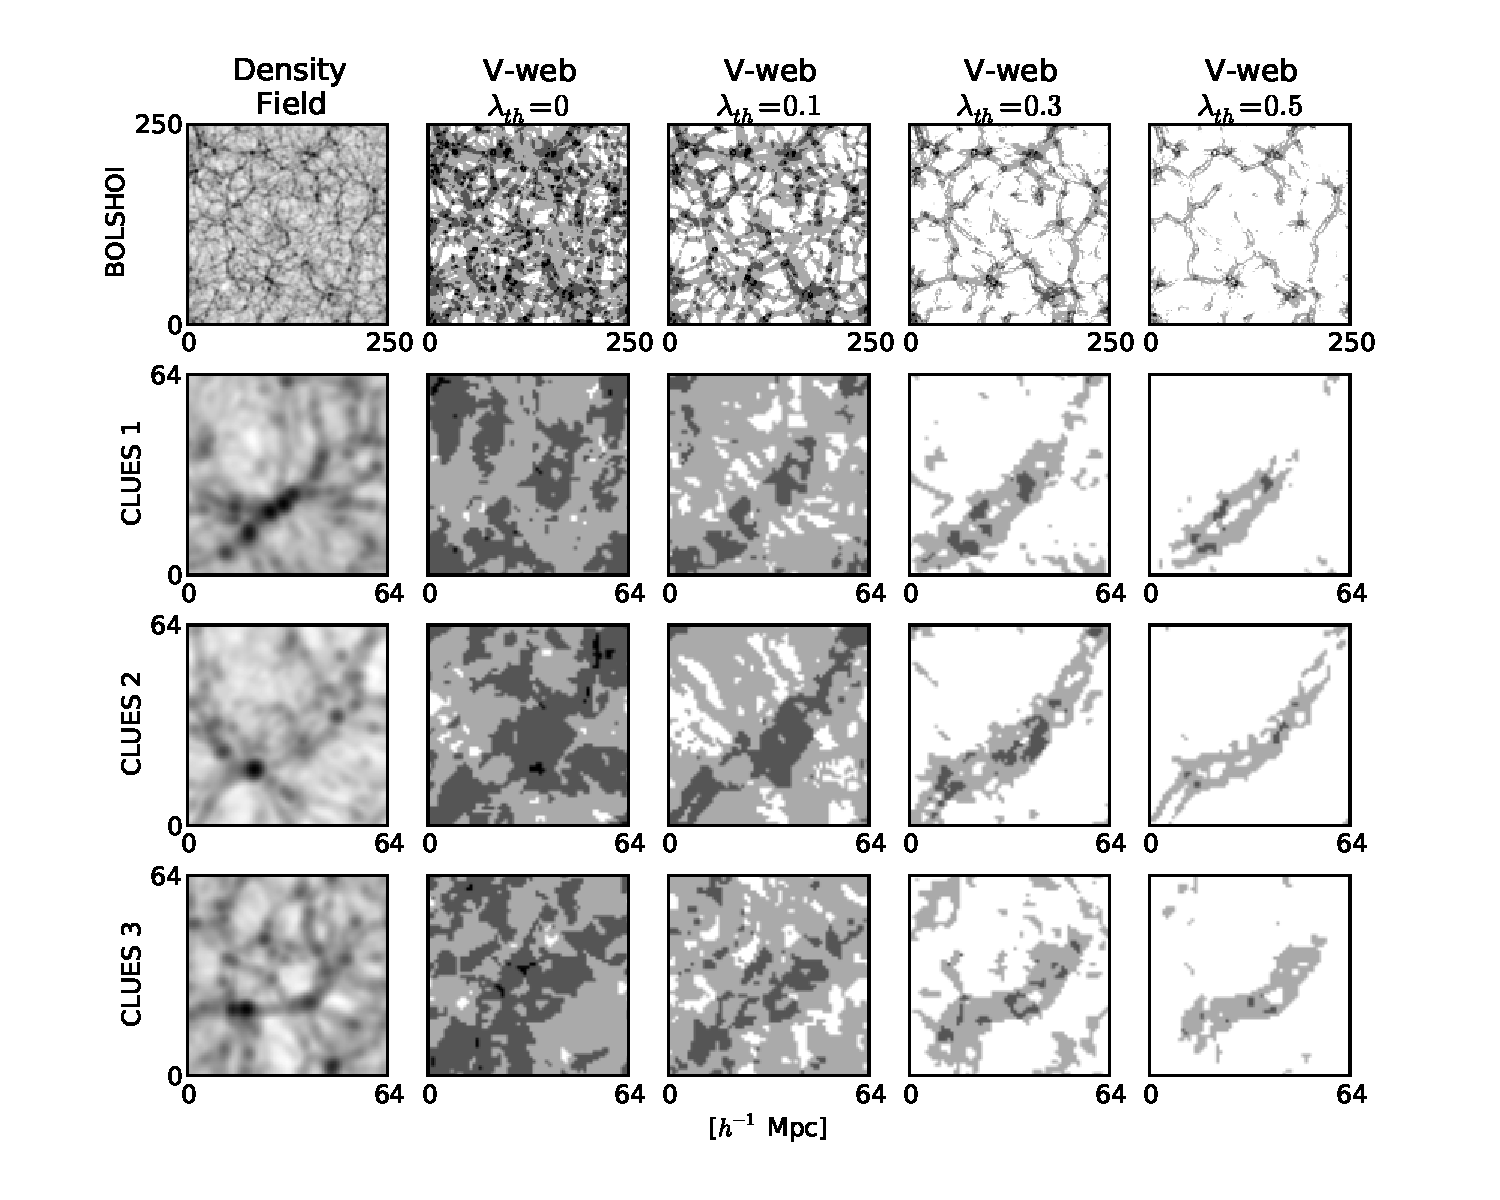
\includegraphics[trim = 10mm 10mm 10mm 9mm, clip,
	width=0.66\paperwidth,angle=0]
	{./figures/4_results/Vweb_Comparison.pdf}}
	\end{center}	
	
	\caption{\small{Comparación de la impresión visual obtenida con el  
	método V-web para varios valores del parámetro $\lambda_{th}$.
	Se usa el siguiente esquema de clasificación (Negro - Nudo, Gris 
	oscuro - Filamento, Gris - Hoja, Blanco - Vacío). La resolución de 
	cada malla es $1.0 h^{-1}$ Mpc/celda, con un suavizado Gaussiano de 
	una celda. El grosor de cada slide es de una celda.}}
	\label{fig:Vweb_Comparison}
\end{figure}
%.........................................................................


Un segundo resultado de la figura \ref{fig:Vol_Fraction} consiste en la 
determinación de un parámetro $\lambda_{th}$ óptimo para la reproducción 
visual de la red cósmica. Como se muestra en esta gráfica, las fracciones
de volumen asociadas a vacíos y hojas son relativamente altas respecto a 
las de filamentos y nudos, esto para todo el rango barrido de valores de 
$\lambda_{th}$. De esto se espera que la impresión visual a gran escala
del campo de materia sea completamente dominada por la distribución de 
vacíos y en menor medida por la distribución de hojas y filamentos. En el 
caso de un valor bajo del parámetro $\lambda_{th}$, por ejemplo 
$\lambda_{th}<0.2$, el parámetro de densidad media de las hojas es negativo, 
indicando que posiblemente estas regiones están invadiendo zonas que deberían 
ser vacíos, tal como se ve en la figura \ref{fig:Vweb_Comparison} para 
$\lambda_{th} = 0$ o $\lambda_{th} = 0.1$. En el caso de valores altos, 
$\lambda_{th} > 0.4\sim 0.5$, el parámetro de densidad medio para los vacíos 
comienza a aumentar, indicando que estas regiones están invadiendo zonas
que de mayor densidad, que en principio deberían ser hojas o filamentos. 
Esto puede ser notado en la figura \ref{fig:Vweb_Comparison} para 
$\lambda_{th} = 0.5$, donde todo el volumen es ampliamente dominado por 
vacíos, perdiendo la estructura característica de la red cósmica. Este 
análisis sugiere que el valor óptimo de $\lambda_{th}$ podría ser aquel 
donde se minimice la densidad media de los vacíos, al ser estos el entorno
dominante. Un resultado que apoya este criterio es que el $\lambda_{th}$ 
encontrado es similar para ambas simulaciones $\lambda_{th}\approx 0.3$,
y coincide con el valor obtenido a partir de un análisis cualitativo de 
la impresión visual del entorno.

\

Para concluir esta sección se discuten los resultados obtenidos para las 
distribuciones de entorno. A pesar de existir un notable sesgo entre
la distribución de los halos y la del campo de densidad en la simulación 
Bolshoi, caso contrario a las simulaciones CLUES, y haber una marcada 
diferencia entre las densidades medias de las regiones en ambas 
simulaciones, la esencia de construir una muestra \textit{CLG} en la 
simulación Bolshoi a partir de los grupos locales de las CLUES, como se 
menciona en el capítulo \ref{cha:N-BodySimulations}, es obtener una muestra 
de pares aislados más fiel que también reproduzcan el entorno local de los 
\textit{LG}. Se espera entonces que la dinámica local cuantificada por la 
V-web se independiente del diferente resultado global de las distribuciones,
manteniéndose así la validez del esquema de construcción de los \textit{CLG}.


%*************************************************************************




%*************************************************************************
%Properties of sample pairs
\section{Propiedades de la Muestra \textit{CLG}}
\label{sec:PropertiesOfSamplePairs}


Una vez determinada la consistencia entre las muestras definidas en CLUES
y Bolshoi, el siguiente paso es determinar sus propiedades. Es de especial
interés analizar la muestra \textit{CLG} de Bolshoi, tomando como muestra 
de control la \textit{IP} y como muestra de referencia la \textit{LG} de 
las simulaciones CLUES.


	%---------------------------------------------------------------------
	%Determination of their host environment
	\subsection{Determinación del Entorno}
	\label{subsec:DeterminationOfTheirHostEnvironment}
	%---------------------------------------------------------------------

Como fue definido en la subsección \ref{subsec:SampleOfPairsToUse} del 
capítulo pasado, la muestra \textit{CLG} en la simulación Bolshoi se 
construye imponiendo a la muestra \textit{IP} la condición extra de 
reproducir el entorno cosmológico de los grupos locales de las simulaciones 
CLUES. La principal motivación de esto es encontrar una muestra en Bolshoi 
análoga a las muestras \textit{LG}, tanto en sus propiedades físicas 
como en su abundancia. Respecto a esto último es natural asumir, 
considerando la ya determinada consistencia entre las simulaciones, que la 
abundancia escala aproximadamente como el volumen simulado. Esto puede 
ser considerado el primer logro de este esquema, ya que reproduce 
aproximadamente esta ley de escalamiento para el tamaño de las muestras 
en cuestión (ver tabla \ref{tab:Samples} para \textit{CLG} de Bolshoi y
\textit{LG} de CLUES).


A pesar de lo anterior, este método de construcción no es más que corte
de la muestra \textit{IP} respecto a los autovalores de la V-web de la 
celda donde están embedidos, lo cual no implica la reproducción 
adecuada de las propiedades físicas ni el entorno cosmológico de los 
sistemas tipo grupo local. Por esta razón, a conti\-nuación son analizados
posibles sesgos producidos en las distribuciones del entorno cosmológico
para los sistemas \textit{CLG}.

	
%.........................................................................
%Pathogenic Situation
\begin{figure}[htbp]
	\centering
	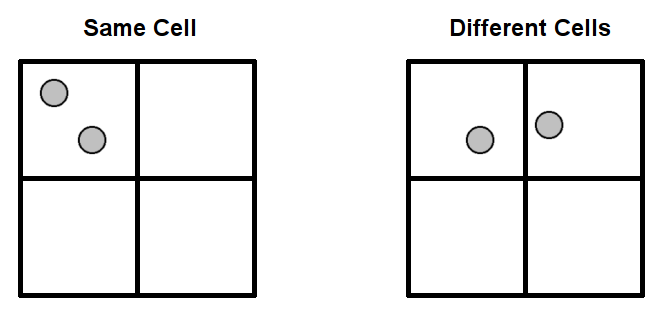
\includegraphics[width=0.5\textwidth]
	{./figures/4_results/Pathogenic_Situation.png}
	
	\caption{\small{Situación patológica respecto al entorno de los sistemas
	de pares de halos.}}
	\label{fig:Pathogenic_Situation}
\end{figure}
%.........................................................................


Una de las primeras consideraciones que debe tenerse en cuenta en la 
cuantificación del entorno para pares de halos (muestras \textit{P}, 
\textit{IP}, \textit{CLG} y \textit{LG}), es que cada uno de ellos puede 
estar embebido en celdas diferentes, tal como es mostrado en la figura 
\ref{fig:Pathogenic_Situation}. Esta situación patológica se presenta debido 
al carácter no puntual de este tipo de sistemas y el tamaño finito de la malla.

\
%.........................................................................
%Comparison of Lambda in each Halos of Pairs systems
\begin{figure}[htbp]
	\centering
	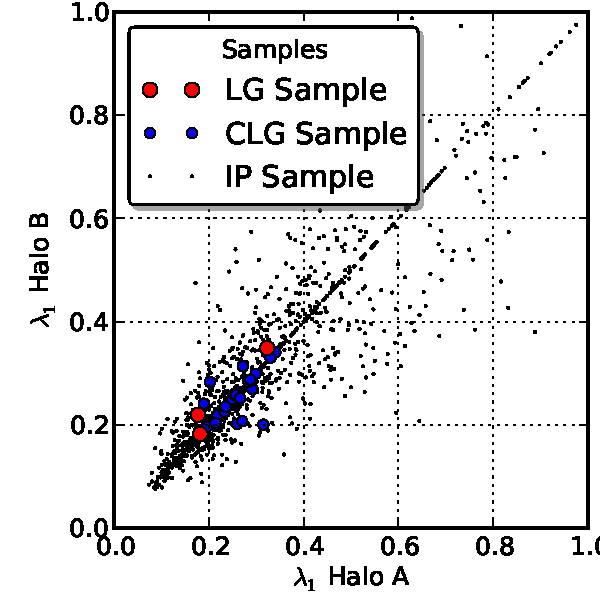
\includegraphics[width=0.46\textwidth]
	{./figures/4_results/CLG_L11_L12.pdf}
	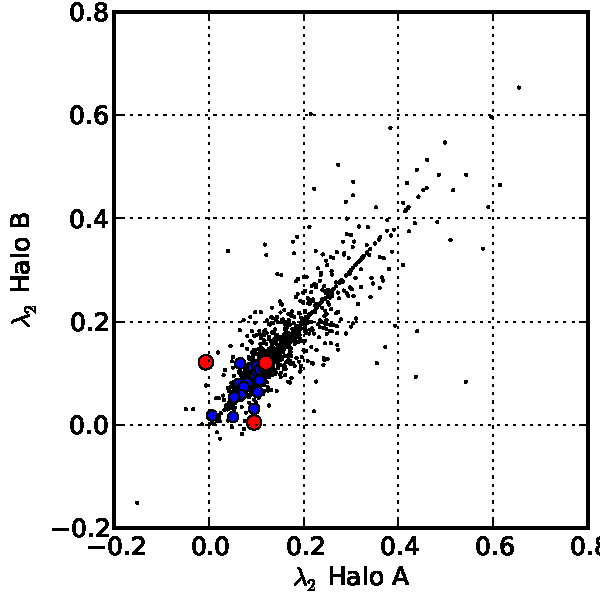
\includegraphics[width=0.46\textwidth]
	{./figures/4_results/CLG_L21_L22.pdf}
	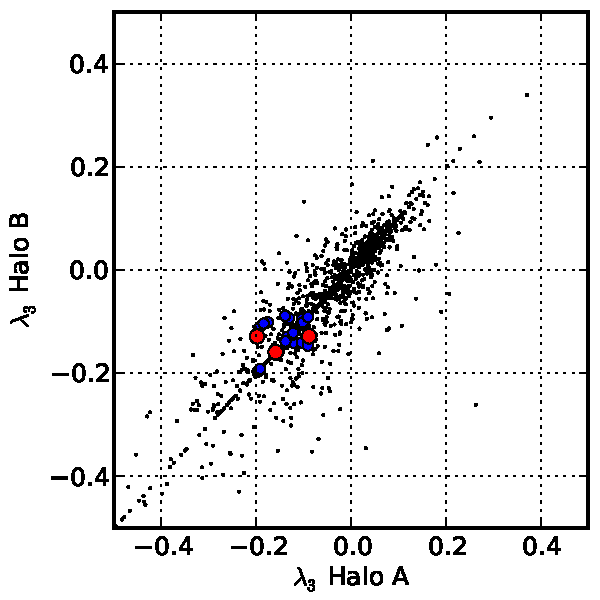
\includegraphics[width=0.46\textwidth]
	{./figures/4_results/CLG_L31_L32.pdf}

	\caption{\small{Comparación entre las distribuciones de los autovalores de 
	la V-web para los dos halos en los sistemas de pares (muestras \textit{LG},
	\textit{CLG} y \textit{IP}).}}
	\label{fig:Lambda_Comparison_Pairs}
\end{figure}
%.........................................................................


Para cuantificar este efecto, en la figura \ref{fig:Lambda_Comparison_Pairs}
son graficadas las distribuciones de cada uno de los autovalores de la V-web
para cada halo de las muestras de pares. La situación ideal, donde ambos
halos comparten una misma celda, correspondería a un línea perfecta 
con pendiente de $45^o$, mientras las situaciones patológicas son responsables 
de dispersiones en las gráficas. Una manera de solucionar esto es disminuir la
resolución de la malla tal que ambos halos estén embebidos en una misma celda, 
pero esto ocasiona una perdida de información del entorno local propio del 
sistema. Debido al suavizado Gaussiano de una celda ($\sim 1 h^{-1}$ Mpc) 
que es aplicado a priori a cada campo de autovalores, la variación de estos 
entre celdas vecinas es menor, tal como es mostrado para la mayoría de 
sistemas \textit{IP} en la gráfica. Teniendo en cuenta esto último y que la 
dinámica local de los pares estará dominada por el halo más masivo, por 
convención será tomada la celda asociada a este halo para la cuantificación
del entorno de todo el sistema.

\
%.........................................................................
%2D Distribution of Vweb eigenvalues in sairs samples
\begin{figure}[htbp]
	\centering
	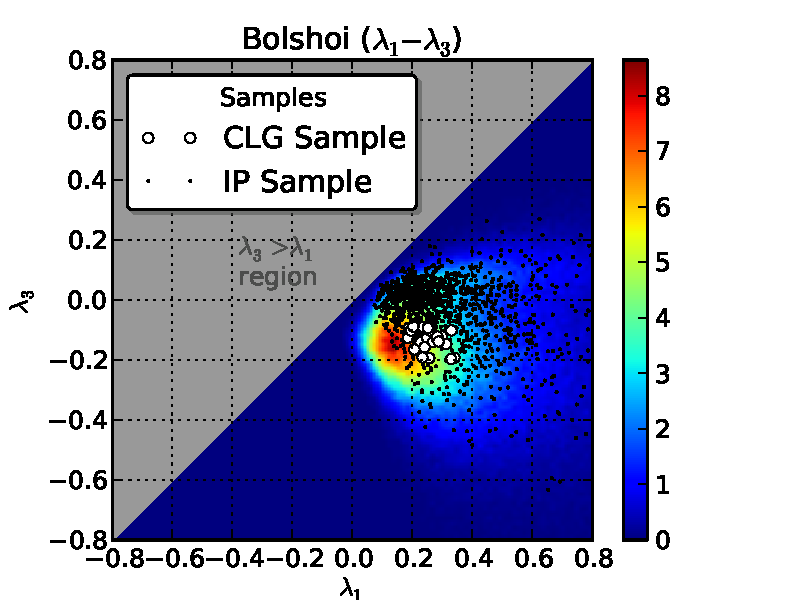
\includegraphics[trim = 0mm 0mm 15mm 0mm, clip, width=0.49\textwidth]
	{./figures/4_results/CLG_Environmet_L1L3.pdf}
	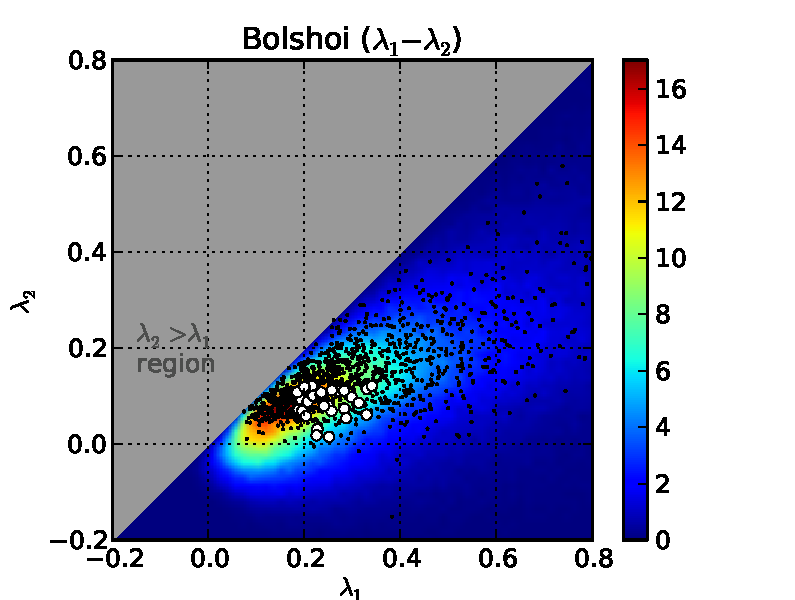
\includegraphics[trim = 0mm 0mm 15mm 0mm, clip, width=0.49\textwidth]
	{./figures/4_results/CLG_Environmet_L1L2.pdf}
	
	\caption{\small{Distribuciones 2D del entorno cosmológico para 
	diferentes muestras, $\lambda_1$--$\lambda_3$ (izquierda) y 
	$\lambda_1$--$\lambda_2$ (derecha). El histograma de fondo, graficado
	en colores, corresponde a la distribución de entorno para todos los 
	halos de Bolshoi (muestra \textit{GH}), su resolución es de $100\times 100$ 
	para el rango mostrado y están normalizados respecto a su área. Los 
	puntos negros corresponden a la distribución de la muestra \textit{IP} 
	y finalmente los puntos blancos a la muestra \textit{CLG}.}}
	\label{fig:2D_Samples_Eigenvalues}
\end{figure}
%.........................................................................


Una vez determinada la forma de cuantificar el entorno de los sistemas de
pares, en la figura \ref{fig:2D_Samples_Eigenvalues} se ilustra la 
distribución de las muestras \textit{GH}, \textit{IP} y \textit{GCL}.
Como fue mostrado en la subsección \ref{subsec:Environment_Properties}, 
la distribución de entorno de los halos en Bolshoi está considerablemente
sesgada respecto a la distribución de las celdas de volumen. A pesar de 
esto y teniendo en cuenta que la construcción de los sistemas de pares se 
hace a partir de los halos, es más interesante realizar comparaciones con las 
distribuciones asociadas a los halos (histogramas de color en la misma figura).
Como fue definido en la subsección \ref{subsec:SampleOfPairsToUse}, la 
muestra \textit{IP} es construida de tal forma que se garantice su
aislamiento gravitacional respecto a halos más masivos, por esta razón hay
dos efectos que compiten en cuanto a la distribución de entorno de estos 
sistemas. En el primero se espera que la abundancia de pares sea más 
favorable en entornos donde la cantidad de halos es mayor, mientras en el
segundo, precisamente la sobreabundancia de halos resulta desfavorable para
los criterios de aislamiento gravitacional. El segundo efecto termina siendo
dominante y produce un sesgo en la distribución de entorno
de la muestra \textit{IP} respecto a la de los halos, mientras que para en 
la muestra \textit{P} el sesgo no se presenta\footnote{Esto 
último no es mostrado en la figura \ref{fig:2D_Samples_Eigenvalues}, pero
es fácilmente calculado.}. 


Para terminar el análisis de la anterior figura, se discute acerca de la 
distribución de entorno para los \textit{CLG} de la simulación Bolshoi. A 
pesar de que esta distribución es construida de forma artificial por 
efecto de selección, es interesante notar que la región en el espacio de 
autovalores que delimita esta muestra es relativamente reducida, indicando 
que los tres grupos locales de las simulaciones CLUES comparten una 
dinámica de entorno local muy similar. Aunque esto último puede ser un 
efecto impuesto a priori por construcción debido al carácter restringido 
de las simulaciones CLUES, no deja de ser interesante el sesgo que esta 
característica produce en la distribución de entorno de los \textit{CLG} 
respecto a los halos y a la muestra \textit{IP}.


Para cuantificar los sesgos producidos en cada muestra respecto a un tipo
de entorno específico (ver figura \ref{fig:ClassificationSchemeTweb}),
en la siguiente figura \ref{fig:Samples_Fraction} se grafican las 
fracciones de objetos en las diferentes regiones. En el rango óptimo del 
valor umbral $0.2\leq \lambda_{th}\leq 0.4$ definido en la subsección 
\ref{subsec:Environment_Properties}, se notan importantes diferencias entre
cada una de las muestras, especialmente para la \textit{CLG}. Como fue 
mencionado anteriormente, el efecto de aislamiento gravitacional produce
un sesgo entre la distribución de entorno de los halos \textit{GH} y de los 
sistemas \textit{IP}, esto puede ser claramente notado para cada una de las 
fracciones en el rango óptimo de $\lambda_{th}$. En el caso de vacíos, la 
fracción dominante de estas dos muestras es la asociada a \textit{IP}, pero 
en el caso de hojas ambas son comparables, y más aún, en la regiones tipo 
filamento y nudo domina la fracción de halos \textit{GH}. Esto indica que
los sistemas de pares aislados \textit{IP} se presentan con mayor 
abundancia en regiones de media o baja densidad de halos, aún así la 
considerable fracción de estos presentes en hojas y filamentos no permite 
asociar un tipo de región de entorno específica para estos sistemas. 
Finalmente, los sistemas \textit{CLG} presentan un importante sesgo 
en comparación a las dos muestras anteriores, siendo de especial interés 
aquella producida respecto a la \textit{IP} debido a que \textit{CLG} es 
una submuestra de esta. De nuevo, apelando al rango óptimo de $\lambda_{th}$,
es posible en este caso asociar tipos de regiones de entorno específicas 
a la muestra \textit{CLG}, estando estos sistemas preferencialmente en 
hojas y vacíos.

\
%.........................................................................
%Number Fraction of each sample in differents type of regions
\begin{figure}[htbp]
	\centering
	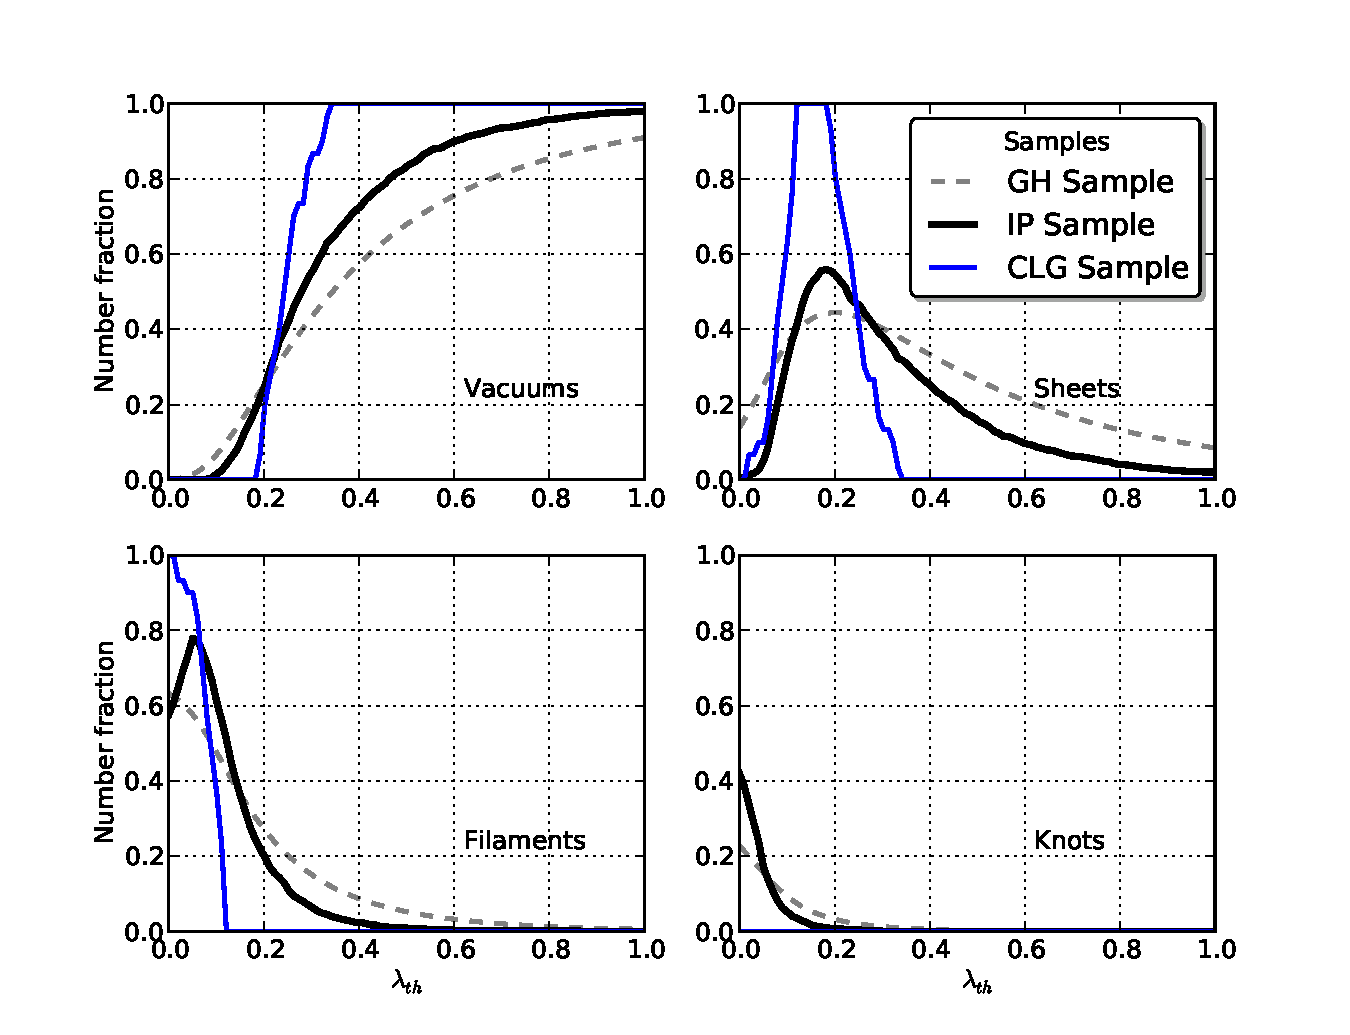
\includegraphics[trim = 8mm 5mm 12mm 12mm, clip, width=0.9\textwidth]
	{./figures/4_results/CLG_Classification_Env.pdf}
	
	\caption{\small{Fracciones de cantidad de objetos en diferentes
	regiones en función del valor umbral $\lambda_{th}$. Para el caso de 
	la muestra \textit{GH} se cuentan número de Halos, mientras que para
	las muestras \textit{IP} y \textit{CLG} número de pares.}}
	\label{fig:Samples_Fraction}
\end{figure}
%.........................................................................


A pesar del esquema de clasificación de regiones usado, las conclusiones 
anteriores dependen de la elección del parámetro $\lambda_{th}$, que aunque
ha sido razonablemente acotado en una región óptima que reproduce la 
impresión visual, no deja de ser un parámetro libre. Para solventar esto se 
introduce el fraccional de anisotropía (FA) con la normalización usada en
\cite{libeskind2013}


%.........................................................................
%Fractional Anisotropy
\eq{eq:FA}
{ FA = \frac{1}{\sqrt{3}}\sqrt{ \frac{ (\lambda_1 - \lambda_3)^2 + 
(\lambda_2 - \lambda_3)^2 + (\lambda_1 - \lambda_2)^2}{ \lambda_1^2 + 
\lambda_2^2 + \lambda_3^2} } }
%.........................................................................


Esta cantidad cuantifica el grado de anisotropía del entorno cosmológico
local, siendo $FA = 1$ una región altamente anisotrópica, mientras
$FA = 0$ un región con alta isotropía, además es independiente de la
elección a priori de algún parámetro libre. Acorde al resultado obtenido por
\cite{libeskind2013}, regiones de baja anisotropía corres\-ponden a nudos
debido a su colapso isotrópico, mientras que regiones de alta anisotropía 
corresponden a vacíos debido a su expansión no uniforme. Para regiones
filamentales y planas el fraccional de anisotropía está distribuido 
de forma extendida en valores intermedios, indicando que la dinámica de
este tipo de entornos es más compleja. Aún así, hay una tendencia a valores
bajos en el caso de filamentos y valores altos para hojas.


%.........................................................................
%Anisotropy Fractional for pairs samples
\begin{figure}[htbp]
	\centering
	\includegraphics[trim = 0mm 0mm 0mm 10mm, clip, width=0.8\textwidth]
	{./figures/4_results/CLG_FA_Hist.pdf}
	
	\caption{\small{Histograma integrado del fraccional de anisotropía para
	las muestras de pares \textit{IP} y \textit{CLG}.}}
	\label{fig:FA_samples}
\end{figure}
%.........................................................................	


En la figura \ref{fig:FA_samples} son calculados los histogramas integrados
del fraccional de anisotropía para las muestras \textit{IP} y \textit{CLG}.
El primer resultado está asociado a la distribución de los \textit{IP}, 
la cual es altamente homogénea para rangos intermedios (aproximadamente 
$0.4 < FA < 0.9$) como es evidenciado en la pendiente constante del 
histograma. Esto implica que los sistemas \textit{IP} están distribuidos
en zonas de media a alta anisotropía, en concordancia con las fracciones 
encontradas en regiones de vacío, hojas y filamentos. El segundo resultado
es el sesgo obtenido en la distribución de FA de la muestra \textit{CLG}.
A diferencia de los \textit{IP}, esta distribución se encuentra concentrada 
en regiones de alta anisotropía (aproximadamente $0.8 < FA < 1.0$), lo que
confirma finalmente que es posible asociar un tipo de entorno cosmológico a 
los sistemas \textit{CLG} y el cual esta acorde con regiones vacías y 
planas, o en términos de las direcciones definidas en la V-web, regiones 
que se expanden en dos direcciones (asociadas a los autovalores 
$\lambda_2$ y $\lambda_3$), mientras que poseen un ligero colapso/expansión 
en la tercera dirección (asociada al autovalor $\lambda_1$). 


La principal ventaja de usar el fraccional de anisotropía radica en que 
esta cuantifica en un solo valor la dinámica del entorno cosmológico, 
permitiendo establecer un marco de estudio más natural y directo para 
correlaciones de entorno con cantidades fisicas.


	%---------------------------------------------------------------------
	%Pairs Mass
	\subsection{Masa de los \textit{CLG}}
	\label{subsec:CLG_Mass}
	%---------------------------------------------------------------------
	

Como fue demostrado en la subsección \ref{subsec:Halos_Properties}, la 
distribución de masa de los halos es consistente entre las diferentes
simulaciones, por tanto se espera que todas las muestras, a excepción de 
\textit{CLG} que requiere además del entorno cosmológico, sean también
consistentes entre las simulaciones. Para el estudio de las masas de los
sistemas de pares se propone el uso de dos cantidades, la primera es la
masa total del sistema $M_{tot} = M_A + M_B$ y la segunda es la relación 
de las masas $\chi = M_B/M_A$, donde por convención $M_A$ es el halo más 
masivo.


En la siguiente figura \ref{fig:CLG_Mass} se calculan los histogramas 
integrados para la masa total y la razón de las masas. Se toma la muestra
\textit{IP} como muestra de control, además se muestran los valores 
obtenidos para cada uno de los grupos locales en CLUES.


%.........................................................................
%Integrated Mass Fraction
\begin{figure}[htbp]
	\centering
	\includegraphics[trim = 0mm 0mm 9.5mm 10mm, clip, width=0.45\textwidth]
	{./figures/4_results/IP_IMF.pdf}
	\includegraphics[trim = 0mm 0mm 9.5mm 10mm, clip, width=0.45\textwidth]
	{./figures/4_results/IP_Mass_Ratio.pdf}
	
	\caption{\small{ Funciones de distribución integrada para la masa total
	$M_{A} + M_{B}$ (izquierda) y la razón de las masas $M_B/M_A$ (derecha), 
	de las muestras de pares en Bolshoi. }}
	\label{fig:CLG_Mass}
\end{figure}
%.........................................................................


Una característica interesante de esta figura consiste en los rangos bien 
definidos asociados a la muestra \textit{LG} de CLUES (líneas rojas 
verticales). Esto evidencia que los grupos locales \textit{LG} no solo 
comparten una entorno cosmológico común sino también una distribución de 
masa local. Como posible explicación a esto puede considerase un efecto de 
selección de las muestras en la construcción de las simu\-laciones 
restringidas, mientras que una alternativa optimista sería tomarlo como 
una evidencia de la correlación entre la distribución de masa y el entorno 
local.


Para responder la anterior cuestión se debe analizar la distribución de
los pará\-metros de masa para las demás muestras. En el caso de la masa
total de los \textit{IP}, esta se encuentra distribuida acorde a 
la distribución de masa de los halos (ver figura \ref{fig:IMF}), tal 
como es esperado al no existir ninguna restricción respecto al 
entorno y en el caso de la razón de masas, se obtiene una distribución
completamente homogénea. Ahora, para la muestra \textit{CLG}, la cual se 
espera que sea influenciada por los efectos del entorno, se obtiene una 
distribución de masa total sesgada respecto a la de \textit{IP} y centrada 
aproximadamente en el rango definido por los \textit{LG}. Para la 
distribución de la razón de masas de \textit{CLG} también se encuentra 
un comportamiento uniforme teniendo en cuenta la escasez de datos, 
a pesar de esto hay una aparente sobreabundancia en torno al valor medio 
definido por los \textit{LG}, pero nuevamente no hay suficientes datos 
para concluir una posible relación.

\newpage
%.........................................................................
%Dispersion diagram for pairs mass parameters
\begin{figure}[htbp]
	\centering
	\includegraphics[trim = 0mm 0mm 0mm 10mm, clip, width=0.8\textwidth]
	{./figures/4_results/IP_Mass_vs_Ratio.pdf}
	
	\caption{\small{Diagrama de dispersión de los parámetros de masa 
	definidos ($M_{tot}$,$\chi$) para cada una de las muestras de pares.
	Las regiones cuadradas son construidas a partir del valor medio y la
	desviación estándar de la muestra del mismo color.
	La región gris en la parte inferior izquierda corresponde a un corte
	impuesto artificialmente con el rango mínimo de masa de los halos 
	tomados $M_*$ para construir las muestras de pares.}}
	\label{fig:Dispersion_Mass_CLG}
\end{figure}
%.........................................................................


En la figura \ref{fig:Dispersion_Mass_CLG} se muestra un diagrama de 
dispersión para los parámetros de masa de las muestras de pares. Las 
regiones cuadradas representan el valor medio más o menos una desviación
estándar para las parámetros marcados en cada eje, lo que permite comparar
gráficamente las distribuciones. De esta comparación se confirma que el 
criterio de construcción de la muestra \textit{CLG} selecciona masas de 
pares $M_{tot}$ consistente con las masa de los \textit{LG} en las simulaciones 
restringidas, mientras que no hace ninguna selección respecto a la razón 
de masas $\chi$.


Finalmente, con el objetivo de responder si existe un posible efecto de 
entorno en la selección de la masa total obtenida para la muestra 
\textit{CLG}, se calcula en la siguiente figura \ref{fig:CLG_FA_Mass} 
diagramas de correlación entre el fraccional de anisotropía y los parámetros 
de masa.

\
%.........................................................................
%Correlation Mass-FA
\begin{figure}[htbp]
	\centering
	\includegraphics[trim = 25mm 0mm 35mm 10mm, clip, width=1.0\textwidth]
	{./figures/4_results/CLG_FA_Mass.pdf}
	
	\caption{\small{Diagramas de dispersión para el fraccional de 
	anisotropía respecto a los parámetros de masa. El mapa de fondo y las
	curvas de contorno corresponden a número de pares de la muestra 
	\textit{IP}.}}
	\label{fig:CLG_FA_Mass}
\end{figure}
%.........................................................................
\

En el caso de la masa total $M_{tot}$ de la muestra \textit{IP}, puede 
notarse que pares con bajos valores de masa están preferencialmente en 
regiones de alta anisotropía, mientras que pares de masa más alta en 
regiones de anisotropía intermedia. Esto puede ser considerado como una 
correlación de entorno para la muestra \textit{IP} respecto a la masa total, 
de lo cual se concluye que el criterio de selección de la muestra \textit{CLG}
a partir del entorno de los \textit{LG} hace un corte para pares de baja 
masa.


Para la razón de las masas $\chi$ se nota una distribución más dispersa 
para la muestra \textit{IP}, a pesar de esto se nota una sobreabundancia 
de pares con valores de $\chi$ bajos en zonas de anisotropía media, 
mientras que en regiones de alta anisotropía se presentan valores más altos
de $\chi$. Esto es consistente con la selección realizada en la muestra
\textit{CLG}, para la cual aproximadamente el $66\%$ de los pares tienen
un valor $\chi>0.5$. De esto puede intuirse una posible correlación entre
el entorno y el valor $\chi$ de los pares, aún así, debido a la alta 
dispersión de la distribución y la poca cantidad de datos, no puede 
concluirse nada al respecto.
\newpage

	%---------------------------------------------------------------------
	%Angular momentum and energy
	\subsection{Distribuciones de Energía y Momentum Angular}
	\label{subsec:AngularMomentumAndEnergy}
	%---------------------------------------------------------------------


La energía y el momentum angular constituyen otras propiedades físicas de
interés para los sistemas de pares, estas son definidas acá a partir de las
siguiente expresiones


%.........................................................................
%Energy of Pairs
\eq{eq:EnergyPairs}
{ e_{tot} = \frac{1}{M_A + M_B}\cor{ \frac{1}{2}\pr{ M_A v_A'^2 + M_B v_B'^2 } 
 - G\frac{M_A M_B}{| \bds r_A' - \bds r_B' |}}
 }
%.........................................................................


%.........................................................................
%Angular Momentum of Pairs
\eq{eq:AMomentumPairs}
{ \bds L_{orb} = \frac{1}{M_A + M_B}\cor{ M_A\bds r_A' \times \bds v_A' + 
M_B\bds r_B' \times \bds v_B' }}
%.........................................................................
donde $\bds r_i'$ es la posición comóvil del halo $i$ y $\bds v_i'$ es la 
velocidad total\footnote{Velocidad total debido a que se incluye la velocidad 
peculiar y el flujo de Hubble respecto al centro de masa del sistema, así 
$\bds v_i' = \bds v_{pec,i} + H_0 \bds r_i'$. } respecto al centro de 
masa del par.


%.........................................................................
%Energy-AMomentum Dispersion
\begin{figure}[htbp]
	\centering
	\includegraphics[trim = 8mm 0mm 25mm 10mm, clip, width=0.8\textwidth]
	{./figures/4_results/CLG_E_vs_L.pdf}
	
	\caption{\small{Diagrama de dispersión para la energía total y el 
	momentum angular orbital de los sistemas de pares. El mapa de fondo
	corresponde a la distribución de la muestra \textit{P}, mientas las
	líneas de contorno a la distribución de la muestra \textit{IP}, en 
	ambos casos los valores corresponden al número de pares. }}
	\label{fig:CLG_E-L}
\end{figure}
%.........................................................................	


En la figura \ref{fig:CLG_E-L} se muestran las distribuciones de energía 
total específica y momentum angular orbital específico para las diferentes 
muestras. Lo primero que puede ser notado es un significativo sesgo entre
la distribución de los \textit{IP} respecto a los \textit{P}, lo que 
demuestra que el criterio de aislamiento gravitacional definido en la 
subsección \ref{subsec:SampleOfPairsToUse} selecciona un rango de energía 
y momentum angular más bajo que en los pares generales, siendo así estos 
sistemas gravitacionalmente más ligados. En el caso de la muestra 
\textit{CLG}, su distribución parece seguir la de los \textit{IP},
no habiendo así una aparente selección por la condición entorno. Por último,
es interesante observar nuevamente que las propiedades asociadas a la
muestra \textit{LG} poseen valores muy cercanos, indicando así que
representan un tipo de sistema bien definido, aunque como ha sido mencionado,
esto puede ser efecto de selección en la construcción de CLUES.

\
%.........................................................................
%Correlation Energy, L_orb-FA
\begin{figure}[htbp]
	\centering
	\includegraphics[trim = 20mm 0mm 35mm 10mm, clip, width=1.0\textwidth]
	{./figures/4_results/CLG_FA_E-L.pdf}
	
	\caption{\small{Diagramas de dispersión para el fraccional de 
	anisotropía respecto a la energía y el momentum angular. El mapa de 
	fondo y las curvas de contorno corresponden a número de pares de 
	la muestra 	\textit{IP}.}}
	\label{fig:CLG_FA_E-L}
\end{figure}
%.........................................................................


En la figura \ref{fig:CLG_FA_E-L} se calculan diagramas de correlación de
la energía y el momentum angular con el fraccional de anisotropía con el 
objetivo de determinar posibles correlaciones. En el caso de la energía
específica, sistemas de pares \textit{IP} con mayor energía (menos ligados) 
parecen estar mayoritariamente en zonas de alta anisotropía, mientras que
sistemas de menor energía (más ligados) están en zonas de anisotropía media,
lo que muestra una correlación entre estas dos cantidades. Para sistemas
\textit{CLG}, la selección a partir del entorno parece sesgar su 
distribución de energía a valores más altos que la distribución media de los
\textit{IP}, lo que es consistente con la correlación encontrada. En este
caso, los sistemas \textit{LG} parecen no seguir esta correlación, teniendo
valores mucho más bajos de energía que lo esperado. Finalmente, para la 
distribución de momentum angular específico no existe ninguna correlación 
clara, siendo cualquier valor $L_{orb}$ de los pares igualmente probable 
en el espectro de posibles entornos para estos sistemas.


	
	%---------------------------------------------------------------------
	%Alineación del momentum angular
	\subsection{Alineación del Momentum Angular}
	\label{subsec:AngularMomentumAlineation}
	%---------------------------------------------------------------------
	
	
Finalmente la última propiedad analizada para los sistemas de pares es su
alineación respecto al entorno cosmológico, para esto se define el ángulo
$\phi_i$ como el formado entre el autovector $\bds u_{\lambda i}$ de la
V-web y el momentum angular del par $\bds L_{orb}$.

	
%.........................................................................
%CLG Alineation
\begin{figure}[htbp]
	\centering
	\includegraphics[trim = 0mm 0mm 5mm 0mm, clip, width=1.0\textwidth]
	{./figures/4_results/CLG_Alineation.pdf}
	
	\caption{\small{Histogramas integrados para el ángulo formado entre el 
	momentum angular de los pares, el cual determina el plano orbital, y
	cada uno de los autovectores definidos por la V-web en el entorno
	cosmológico. Se realiza para cada las muestras de pares \textit{CLG} y 
	\textit{IP}, mientras que los grupos locales de CLUES son ilustrados 
	con las líneas rojas punteadas.}}
	\label{fig:CLG_Alineation}
\end{figure}
%.........................................................................
	

En la figura \ref{fig:CLG_Alineation} se calculan los histogramas 
integrados para cada uno de los angulos $\phi_i$ definidos. Como puede 
notarse, las muestras \textit{CLG} y \textit{IP} son homogéneas respecto
a los tres valores, indicando que no hay una alineación preferida respecto
al entorno cosmológico. Esto también se evidencia en los valores calculados
de los \textit{LG} de las simulaciones restringidas.


%*************************************************************************



	
%*************************************************************************
%Conclusions
\section{Conclusiones}
\label{sec:Conclusions}


Esta sección está dedicada a compilar los principales resultados obtenidos
en este capítulo. Estos serán enumerados y discutidos acorde al órden en
que fueron obtenidos.


%.........................................................................
%Main Results
\begin{enumerate}
\item[\textbf{1.}] La construcción de la muestra \textit{IP} fue 
inicialmente propuesta en \cite{forero2011} con el objetivo de reproducir
sistemas tipo grupo local. A pesar de esto, el número de estos sistemas 
encontrados en la simulación Bolshoi es mucho mayor al que se espera acorde
a la abundancia de \textit{LG} en simulaciones restringidas. El método 
propuesto para la selección de la muestra \textit{CLG} en Bolshoi a partir 
del entorno cosmológico de los \textit{LG}, produce un número de sistemas 
que concuerda con los encontrados en la simulaciones restringidas, escalando 
apro\-ximadamente como el volumen de las simulaciones. Más aún, aplicando 
este mismo método en las simulaciones restringidas se halla una muestra
con un tamaño similar a la \textit{LG}.


\item[\textbf{2.}] A partir de los valores medios de densidad en las 
diferentes regiones del entorno cosmológico (figura \ref{fig:Vol_Fraction})
se propone un esquema para la elección de un rango óptimo del parámetro
$\lambda_{th}$ de la V-web con el objetivo de reproducir la 
apariencia visual de la red cósmica. Este está basado en la 
minimización de la densidad media en las regiones de vacío debido a que
son las dominan la apariencia del campo de densidad a gran escala. Con
esto se garantiza que las regiones vacías no invadan regiones de más alta
densidad, que en principio deben ser clasificadas como hojas o filamentos.
Este método da un rango de valores óptimos aproximadamente igual para 
todas las simulaciones usadas ($0.2 \leq \lambda_{th} \leq 0.4$), además
reproduce adecuadamente la apariencia visual (ver figura 
\ref{fig:Vweb_Comparison} para $\lambda_{th} = 0.3$). A pesar de esto, 
este parámetro sigue siendo libre y no es viable usar un esquema de 
clasificación basado en este para determinar correlaciones con propiedades
físicas, en vez de esto se introduce el fraccional de anisotropía 
con la normalización usada en \cite{libeskind2013}.


\item[\textbf{3.}] La distribución del entorno cosmológico de las 
simulaciones Bolshoi y CLUES difieren, existiendo un cambio de densidad 
media muy pronunciado entre regiones de vacío y filamentos en Bolshoi, 
mientras que es mucho más suave en las CLUES. A pesar de esto, las 
fracciones de volumen asociadas a cada tipo de entorno son aproximadamente 
iguales para ambas simulaciones en el rango óptimo determinado para 
$\lambda_{th}$. A pesar de esto, se espera que la dinámica local 
caracterizada por la V-web sea independiente de la estructura global 
de la distribución de entorno, lo cual valida el esquema de selección 
de la muestras \textit{CLG} en Bolshoi.


\item[\textbf{4.}] El método de construcción de los 
\textit{CLG} selecciona un entorno cosmológico común para estos 
sistemas, siendo preferidas zonas de vacío y hojas no muy planas.
Estas regiones presentan una alta anisotropía, cuantificada por el 
fraccional de anisotropía FA. En el caso de los sistemas \textit{IP},
estos se encuentran en zonas de media a alta anisotropía, asociadas 
a valores de baja densidad, contrario a los halos que están en zonas 
más densas y menos anisotrópicas como filamentos y nudos, aún así 
la distribución de entorno de los \textit{IP} es amplia y no pueden
ser asociados a un tipo de entorno específico. El sesgo producido
entre los \textit{IP} y los halos generales se debe al criterio
de aislamiento gravitacional usado para construir los \textit{IP},
esto hace que zonas con mayor densidad de halos sean menos aptas por
la alta influencia gravitacional.


\item[\textbf{5.}] Se encuentra una correlación entre la masa total de 
los pares de la muestra \textit{IP} y el fraccional de anisotropía del 
entorno, donde masas mayores son más abundantes en regiones de 
anisotropía media mientras masas menores se presentan con mayor 
frecuencia en zonas de alta anisotropía. Esto implica que la selección
de entorno realizada en los \textit{CLG} reproduce un rango de masa menor.
En el caso de la razón de masa, no se encuentra ninguna correlación 
significativa con el entorno, aún así se nota una ligera sobreabundancia 
de razones de masa mayores en regiones más anisotrópicas, pero es 
necesaria más estadística para poder ser algo concluyente.


\item[\textbf{6.}] Se halla un correlación para la energía específica
de los sistemas \textit{IP} respecto al entorno, obtiendo valores más
altos en regiones más anisotrópicas y valores bajos en regiones de 
anisotropía media. Esta correlación parece seleccionar un rango de 
energía para los sistemas \textit{CLG}, aunque esta no es consistente
con los valores obtenidos de los \textit{LG}. Para el momentum angular
no se encuentra ninguna correlación con el entorno.


\item[\textbf{7.}] Finalmente se encuentra que no existen alineaciones
privilegiadas entre el momentun angular de los pares \textit{CLG} (o de 
su plano orbital) y las direcciones de los autovectores de la V-web.


\end{enumerate}
%.........................................................................


%*************************************************************************

% --------------------------------------------------------------
%:                  BACK MATTER: appendices, refs,..
% --------------------------------------------------------------

% the back matter: appendix and references close the thesis
\backmatter


%: ----------------------- appendix ------------------------

%\appendix


%: ----------------------- bibliography ------------------------



% The section below defines how references are listed and formatted
% The default below is 2 columns, small font, complete author names.
% Entries are also linked back to the page number in the text and to external URL if provided in the BibTex file.


% Original version:

% PhDbiblio-url2 = names small caps, title bold & hyperlinked, link to page 
%\begin{multicols}{2} % \begin{multicols}{ # columns}[ header text][ space]
%\begin{tiny} % tiny(5) < scriptsize(7) < footnotesize(8) < small (9)
%
%\bibliographystyle{Latex/Classes/PhDbiblio-url2} % Title is link if provided
%\renewcommand{\bibname}{References} % changes the header; default: Bibliography
%
%\bibliography{9_backmatter/references} % adjust this to fit your BibTex file
%
%\end{tiny}
%\end{multicols}



% Show all bibliography entries
%\nocite*



% If we want bibliography backreference, use unsrt first and the desidered one after

%\bibliographystyle{unsrt} % Defines the bibliography style

%\bibliographystyle{alpha} % Defines the bibliography style

%\bibliographystyle{apa-good} % Defines the bibliography style
%\bibliographystyle{natbib} % Defines the bibliography style

%\bibliographystyle{plainurl}

%\renewcommand{\bibname}{References} % changes the header; default: Bibliography

%To include the references/works cited/bibliography in your Table of Contents, right before the bibliography command, use the command
%\addcontentsline{toc}{section}{References}
%
\bibliographystyle{abbrv}
\bibliography{chapters/references} % adjust this to fit your BibTex file


%\printnomenclature[1.5cm] % [] = distance between entry and description

\printnomenclature % [] = distance between entry and description

% --------------------------------------------------------------
% Various bibliography styles exit. Replace above style as desired.

% in-text refs: (1) (1; 2)
% ref list: alphabetical; author(s) in small caps; initials last name; page(s)
%\bibliographystyle{Latex/Classes/PhDbiblio-case} % title forced lower case
%\bibliographystyle{Latex/Classes/PhDbiblio-bold} % title as in bibtex but bold
%\bibliographystyle{Latex/Classes/PhDbiblio-url} % bold + www link if provided

%\bibliographystyle{Latex/Classes/jmb} % calls style file jmb.bst
% in-text refs: author (year) without brackets
% ref list: alphabetical; author(s) in normal font; last name, initials; page(s)

%\bibliographystyle{plainnat} % calls style file plainnat.bst
% in-text refs: author (year) without brackets
% (this works with package natbib)


% --------------------------------------------------------------


%: Declaration of originality

% this file is called up by thesis.tex
% content in this file will be fed into the main document

%: ----------------------- introduction file header -----------------------


% the code below specifies where the figures are stored
\ifpdf
    \graphicspath{{9_backmatter/figures/PNG/}{9_backmatter/figures/PDF/}{9_backmatter/figures/}}
\else
    \graphicspath{{9_backmatter/figures/EPS/}{9_backmatter/figures/}}
\fi

% Thesis statement of originality -------------------------------------

% Depending on the regulations of your faculty you may need a declaration like the one below. This specific one is from the medical faculty of the university of Dresden.

\begin{declaration}        %this creates the heading for the declaration page

I herewith declare that I have produced this work without the prohibited assistance of third parties and without making use of aids other than those specified; notions taken over directly or indirectly from other sources have been identified as such. This work has not previously been presented in identical or similar form to any examination board.

The dissertation work was conducted from 20XX to \the\year \ under the supervision of
Name Surname
and 
Name Surname
at 
the University of Deusto.

\vspace{10mm}

% City
Bilbao,

% Signature figure

%\begin{flushright}
%\begin{figure}[htbp!]
%\end{figure}
%\includegraphics{signature}%
%\end{flushright}


\end{declaration}



%-------------------------------------------------------------------------

\thispagestyle{empty}

\hfill
\vfill
\medskip

\begin{center}
\noindent
This dissertation was finished writing 
in 
Medellín, Colombia
on
% Date
\today 
\end{center}

\vfill
\medskip
\vspace{1cm}
\bigskip


%-------------------------------------------------------------------------

% Blank page
\clearpage
\thispagestyle{empty}

\hfill
\vfill
\medskip

\begin{center}
\textit{This page is intentionally left blank}
\end{center}

\vfill
\medskip
\vspace{1cm}
\bigskip


% ----------------------------------------------------------------------





\end{document}
